%
%
% wabun2025.tex
%
%
%
\documentclass[a4paper,11pt]{article}
\usepackage{amsmath, amssymb, braket} % AMS math
\usepackage{lmodern} % Font for mathematical formulas
\usepackage{graphicx,color} % https://texwiki.texjp.org/?hyperref
\usepackage{subcaption} % captions for figures etc.
\usepackage{bm} % bold math
\usepackage{quantikz} % quantum circuit diagrams
\usepackage[version=4]{mhchem} % chemical formulas
\usepackage[backend=biber, style=numeric, maxnames=5, doi=false, url=true, eprint=true]{biblatex}
\addbibresource{quantum.bib}
\makeatletter
\let\mkbibemph=\mkbibitalic
\let\blx@imc@mkbibemph=\blx@imc@mkbibitalic
\makeatother
\setlength{\biblabelsep}{0.5em}

%\usepackage{pdfx}  % side effect: also configures hyperref
\usepackage{hyperref} % embed links and generate PDF bookmarks
\hypersetup{
    colorlinks=true,
    linkcolor=blue,
    urlcolor=cyan,
    pdftitle={Quantum Circuit for First Quantization Hamiltonian Simulation Handling Coulomb Potential Pole},
    pdfauthor={Hideo Takahashi},
    pdfsubject={Research Paper},
    pdfkeywords={Quantum Computer, First Quantization, ab initio, Simulator, Coulomb Potential, Quantum Chemistry},
    bookmarksnumbered=true,
    bookmarksopen=true
}
\usepackage{paper2025}

\begin{document}
\title
{Time-Evolution Simulation and Error Analysis of\\
1D and 2D Hydrogen-Atom Models Based on First Quantization\\
Implemented with Quantum Circuits}
\author{Hideo Takahashi}
\date{\today}
\maketitle
\begin{abstract}
We construct a quantum-circuit Hamiltonian simulator based on first
quantization that can run on a quantum-computer emulator with a limited number
of qubits, and present a working example. Using a 26-qubit circuit with a
6-bit coordinate register, we realize a simulation of a two-dimensional model
of a single hydrogen atom. To the best of our knowledge, this is the first
reported working example of a grid-based simulator in which all components,
including the Coulomb potential, are implemented in quantum circuits. To reduce
the total qubit count, we use a Uniformly Controlled Rotation (UCR) circuit for
Coulomb-potential evaluation. To obtain accurate results, we examine how to
treat the Coulomb singularity and how to choose discretization parameters. For
the pole of the Coulomb potential, we show (for the two-dimensional model) that
accurate results are obtained by focusing on the average over the near-pole
region and using one quarter of the grid spacing as the effective interparticle
distance in grid cells containing the pole. The grid spacing can be chosen by
balancing the spatial extent of the wavefunction against discretization, which
minimizes simulation error. The time step for Trotter decomposition can be
determined from the maximum wave number in momentum space obtained by Fourier
transforming the wavefunction.

\end{abstract}

\section{Introduction}
Since the early conception of quantum computers, quantum-chemistry simulation
has been viewed as an application area expected to advance substantially with
quantum computing. Current mainstream quantum-computing hardware is inherently
affected by noise-induced computational errors, and practical error-correction
technology is under active development. Surface-code methods, a promising
approach to quantum error correction, require far higher redundancy than
classical error correction. Consequently, practical fault-tolerant quantum
computers (FTQCs) still face major implementation challenges, including a large
increase in hardware qubit counts, and are expected to take several more years
to realize. In today’s NISQ era, where error correction is not yet available
and qubit counts are limited, second-quantized VQE-based algorithms are the
mainstream approach in quantum chemistry. By combining quantum and classical
computing, VQE reduces required qubit counts and circuit depth, and can tolerate
noise, making it executable on NISQ devices. Once FTQC becomes available,
noise effects can be suppressed and qubit constraints relaxed, opening the way
to a broader class of algorithms.

The grid method, a representative first-quantized approach to quantum-chemistry
simulation, directly handles electron interactions without relying on a basis
set choice. It is therefore an ultimate target for quantum-chemistry
simulation, but it requires substantial computational resources. In the grid
method, indices of uniformly spaced grid points are mapped to qubit-register
bit values; wavefunction amplitudes at grid points are stored as register
amplitudes; and time evolution is then computed. Algorithms based on
Suzuki-Trotter decomposition are widely known for time evolution, although other
approaches have also been proposed. Grid-based algorithms generally require many
qubits and deep circuits, and they cannot tolerate computational error, so
demonstrations remain extremely limited. To the best of the author’s knowledge,
there are no reported demonstrations on actual quantum hardware. Existing
reports all use classical quantum-computer emulators. Benenti et al. performed
simulations with a simplified potential function
\cite{Benenti2008.10.1119/1.2894532}. Chan et al. used a quantum emulator
together with a classical program, with Coulomb-potential evaluation performed
classically \cite{Chan2023.sciadv.abo7484}. No report, even on an emulator,
has implemented Coulomb-potential evaluation itself as a quantum circuit. In
this work, we present a working example of a grid-method simulator in which all
components, including Coulomb-potential calculation, are implemented in quantum
circuits. For simulator-circuit generation, we use `crsQ`, developed by the
author \cite{takahashi2024.doi:10.1021/acs.jctc.4c00708}. We implement the
entire grid-based wavefunction time evolution in quantum circuits, run it on a
quantum-computer emulator, and evaluate the results. To this end, we address
the following challenges.

The first challenge is to present a circuit configuration that can run on an
emulator. Because quantum-computer emulators are limited in available qubit
count, we simplify the computational model to fit within emulator capacity,
targeting one-dimensional and two-dimensional single-hydrogen-atom models with
fixed nuclear coordinates. For Coulomb-potential evaluation, we use both a
binary-arithmetic approach and the UCRZ circuit, which is similar to QROM. For
time evolution, we use standard Suzuki-Trotter decomposition. This yields
example circuit configurations that are executable on emulators and may be
useful for early FTQC-oriented baseline evaluations.

The second challenge is to define a treatment of Coulomb-potential
singularities. In the grid method, potential energy must be computed for all
coordinate combinations of all particles and multiplied by wavefunction
amplitudes. These combinations include cases where nuclear and electron
coordinates coincide, i.e., singular points of the Coulomb potential, which
diverge under naive handling. We propose a method based on averaging within a
grid cell and evaluate it numerically.

The third challenge is to determine simulation parameters that minimize error
under a fixed qubit budget. In the grid method, one must first choose the
simulation-domain size and grid spacing. When Suzuki-Trotter decomposition is
used, the time-step interval must also be chosen. Under limited available
qubits, these parameters exhibit trade-offs and dependencies.

\section{Methods}
\subsection{Unit System}

In this section, we use the atomic unit system (a.u.), in which the physical
quantities listed in Table \ref{tab:unit-system} are set to 1.

\begin{table}[ht]
    \centering
    \begin{tabular}{llccc}
        Physical quantity & Physical constant & Symbol & Value in SI units & Value in other units \\
        \hline
        Charge & Elementary charge & $e$ & $1.602\times10^{-19}$ C \\
        Mass & Electron mass & $\melec$ & $9.109\times10^{-31}$ kg \\
        Length & Bohr radius & $a_0$ & $5.292\times10^{-11}$ m & $0.5292$ \AA \\
        Energy & Hartree & $E_h$ & $4.360\times10^{-18}$ J & $27.21$ eV \\
        Time & Atomic unit of time & $\hbar/E_h$ & $2.419\times10^{-17}$ s & $24.19$ attosecond \\
    \end{tabular}
    \caption{Unit system}
    \label{tab:unit-system}
\end{table}


\subsection{Simulator Overview}

The simulator-circuit generator developed in this study can generate circuits
for models with multiple electrons and multiple nuclei. However, in this
section we consider a single-hydrogen-atom model, where the nucleus is fixed at
the origin of the coordinate system. We target one-dimensional and
two-dimensional spaces.

Let the position basis $\{\ket{j}\}$ be an orthonormal basis corresponding to
discrete grid points $\{\chij\}$,
\begin{equation}
\braket{i|j}=\delta_{ij}
\end{equation}
which satisfies

In this case, the state vector in the position representation, $\ketPsiRS$, is
written using the wavefunction amplitude at grid point $j$,
$\Psi_j=\Psi(\chij\deltar)$, as
\begin{equation}
\ketPsiRS = \sum_{j}\Psi_j\ket{j}
\end{equation}
On the other hand, the state vector in the wave-number representation,
$\ketPsiKS$, is written using the plane-wave basis function
$W_{\ell}(\bm{r})=e^{i\bm{k}_{\ell}\cdot\bm{r}}/\sqrt{D^d}$ and the wavefunction
component $\tilde{\Psi}_{\ell}$ at that basis wave number:
\begin{equation}
\Psi(\bm{r})=\sum_{\ell} \tilde{\Psi}_{\ell}W_{\ell}(\bm{r})\leftrightarrow
\ketPsiKS = \sum_{\ell}\tilde{\Psi}_{\ell}\ket{\ell}
\end{equation}
Thus,

For a system in which only electrons are treated quantum mechanically, the
one-step time-evolution circuit $\Thetae$ performs one time-evolution step based
on first-order Suzuki-Trotter decomposition.
\begin{align}
\ket{\Psi(t+\deltat)}
 &= e^{-iH\deltat/\hbar}\ket{\Psi(t)} \notag \\
 &\approx \Thetae \ket{\Psi(t)} \label{eq:circuit-eval-theta-e}\\
 &= \Thetaep\QFT\Thetaek\QFTdagger\ket{\Psi(t)}\\
    \Thetaep&=e^{-i\Hep\deltat/\hbar}\\
    \Thetaek&=e^{-i\Hek\deltat/\hbar}
\end{align}
The kinetic-energy term is evaluated in the wave-number representation, and the
potential-energy term is evaluated in the position representation. In atomic
units, with the nucleus at the origin, these equations simplify as follows for
the one-dimensional and two-dimensional computational models.
\begin{align}
   \HekOneD(\bm{k}) = -\frac{(\hbar\kx)^2}{2}, \qquad &
   \HepOneD(\bm{r}) = -\frac{1}{\abs{x}} \label{eq:HkHp1D}\\
   \HekTwoD(\bm{k}) = -\frac{(\hbar\kx)^2 + (\hbar\ky)^2}{2}, \qquad &
   \HepTwoD(\bm{r}) = -\frac{1}{\sqrt{x^2+y^2}} \label{eq:HkHp2D}
\end{align}

The simulator circuit consists of a qubit initialization circuit $\PsiSD$ and a
time-evolution circuit. The time-evolution circuit repeats the one-step
time-evolution circuit $\Thetae$ for the required number of steps. The
initialization circuit loads the initial wavefunction values into the qubits.
\begin{equation}
\ket{\Psi(t=0)} = \PsiSD \ket{0}
\end{equation}
For this, we use an initial-wavefunction preparation circuit
\cite[Sec. 2.2]{takahashi2024.doi:10.1021/acs.jctc.4c00708}.

\clearpage
\subsection{Computational Model}
For evaluation in this section, we use solutions of the time-independent
Schrodinger equation for one-dimensional and two-dimensional hydrogen-atom
models. Solutions of the time-independent equation are stationary solutions of
the time-dependent Schrodinger equation. Therefore, when such a solution is
used as the initial state and evolved in time, the absolute value of the
amplitude is time-independent and only the phase is time-dependent. The phase
change rate is also obtained from the eigenvalue, which can be used to evaluate
simulation results.

\begin{equation}
H\psi(\bm{r})=E\psi(\bm{r})
\end{equation}
If this equation has multiple eigenvalues $E_n$ and eigenfunctions
$\psi_n(\bm{r})$, i.e.,
\begin{equation}
H\psi_n(\bm{r})=E_n\psi_n(\bm{r}),\quad n=1,2,\ldots
\end{equation}
then the wavefunction of a system initialized with the eigenfunction
corresponding to eigenvalue $E_n$ is
\begin{equation}
\Psi_n(\bm{r},t)=\psi_n(\bm{r})\exp\left(-\frac{iE_nt}{\hbar}\right)
\end{equation}
which is used as a reference expression for comparing simulation results.

Because simulations are performed for one-dimensional and two-dimensional
models, we present the analytical solutions of each model below.

For the one-dimensional model, we use Loudon’s analytical solutions
\cite{Loudon1959.10.1119/1.1934950}. According to Loudon, the ground-state
solution with principal quantum number $n=0$ is a delta function. For $n>0$,
both even and odd solutions are given. In this paper, we use the odd solutions,
which can be handled by Fourier transform. Let the odd solution for quantum
number $n\in{1,2,\ldots}$ be denoted by $\psi_n^{\mathrm{1D}}$.
\begin{equation}
\psi_n^{\mathrm{1D}}(x)=\sqrt{\frac{2}{a_0^3n^5(n!)^2}}
\exp\left(-\frac{\abs{x}}{na_0}\right)xL_n^1\left(\frac{2\abs{x}}{na_0}\right)
\end{equation}
Here, $L_n^k$ is the associated Laguerre polynomial. The corresponding energy
eigenvalue is given, for $n\in{1,2,\ldots}$, by
\begin{equation}
    E_n^{\mathrm{1D}}=-\frac{\hbar^2}{2\melec a_0^2 n^2}
\end{equation}
For evaluation, we use the $n=1$ wavefunction $\psi_1^{\mathrm{1D}}$:
\begin{align}
\psi_1^{\mathrm{1D}}(x)&=\sqrt{2}e^{-\abs{x}} x
\label{eq:psi1D1-wave-function}\\
E_1^{\mathrm{1D}}&=-\frac{1}{2}
\label{eq:psi1D1-energy}
\end{align}

The position and wave-number representations of $\psi_1^{\mathrm{1D}}$ are shown
in Figure \ref{fig:initial-wavefunction-1d}.

\begin{figure}[ht]
    \centering
    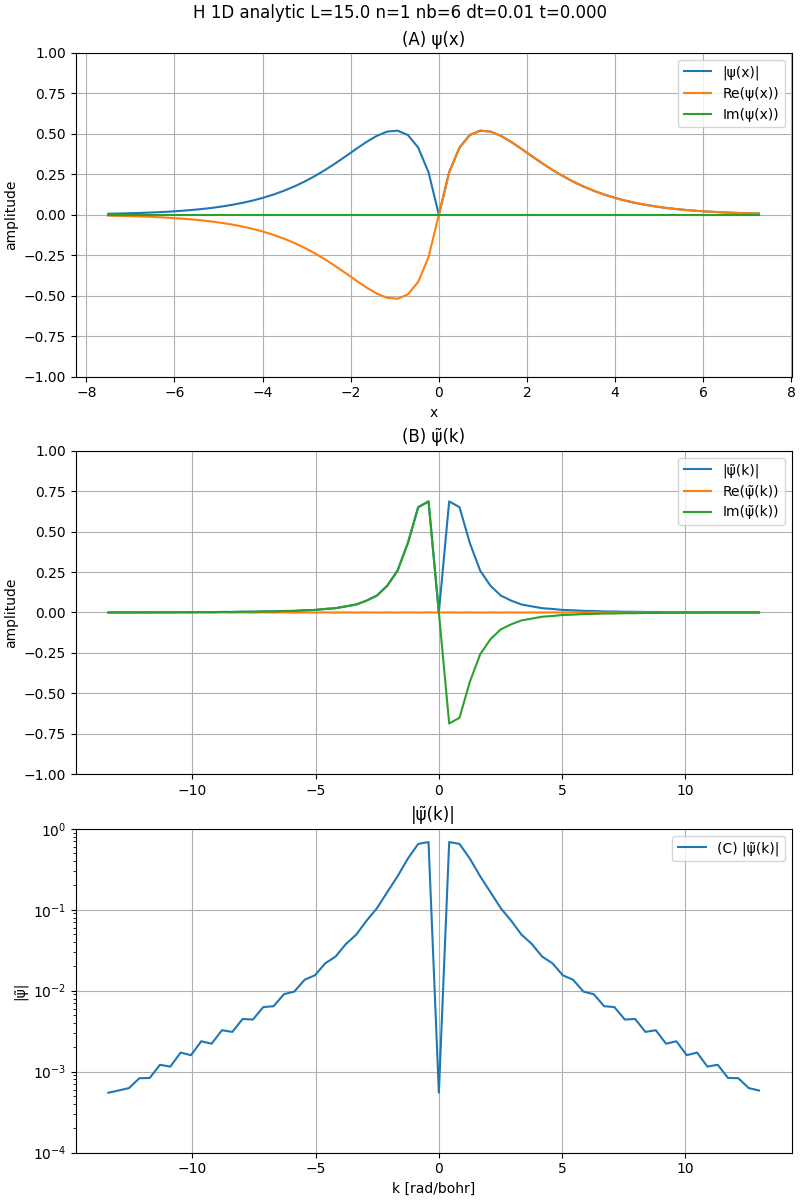
\includegraphics[width=0.6\textwidth]{paper2025_figs/analytic1D/t_00.000.png}
    \caption{Example wavefunction $\PsiOneD_1$ for the one-dimensional model}
    \label{fig:initial-wavefunction-1d}
    \begin{flushleft}\small

        Values of $\PsiOneD_1$ at 6-bit resolution
        (Eq. \eqref{eq:psi1D1-wave-function}).
        (A) Wavefunction amplitude in real space.
        (B) Wavefunction amplitude in k-space.
        (C) Log-scale plot of k-space amplitude.

    \end{flushleft}
\end{figure}

For the two-dimensional model $\psi_{n,\ m}^{\mathrm{2D}}$, we use Parfitt’s
analytical solution \cite{Parfitt2002.10.1063/1.1503868}. This model constrains
an electron moving under the Coulomb potential $-1/\sqrt{x^2+y^2}$ to a
two-dimensional plane. The wavefunction has two quantum-number parameters,
$n\in\{0,\ldots\}$ and $m\in\{-n,\ldots,0,\ldots,n\}$.
\begin{equation}
\psi_{n,\ m}^{\mathrm{2D}}(r,\ \theta)=
\sqrt{\frac{q_0^3(n-\abs{m})!}{\pi(n+\abs{m})!}}(2q_0r)^{\abs{m}}
e^{-q_0r}L_{n-\abs{m}}^{2\abs{m}}(2q_0r)e^{im\theta}
\end{equation}
Here, $q_0=1/(n+1/2)$. The energy eigenvalue is given, for
$n\in\{0,\ldots\}$, by
\begin{equation}
E_n^{\mathrm{2D}}=-\frac{1}{2(n+1/2)^2}
\end{equation}
For evaluation, we use the ground state $\psi_{0,0}^{2D}$ and excited states
$\psi_{1,0}^{2D}$ and $\psi_{1,1}^{2D}$.
\begin{align}
\psi_{0,0}^{\mathrm{2D}}(r,\theta)&=\sqrt{\frac{8}{\pi}}e^{-2r}
\label{eq:psi2D00-wave-function}\\
E_0^{\mathrm{2D}}&=-2
\label{eq:psi2D00-energy}\\
\psi_{1,0}^{\mathrm{2D}}(r,\theta)&=\sqrt{\frac{8}{27\pi}}(1-\frac{4}{3}r)e^{-\frac{2}{3}r} 
\label{eq:psi2D10-wave-function}\\
\psi_{1,1}^{\mathrm{2D}}(r,\theta)&=\frac{8}{9\sqrt{3\pi}}re^{-\frac{2}{3}r+i\theta}
\label{eq:psi2D11-wave-function}\\
E_1^{\mathrm{2D}}&=-\frac{2}{9}\simeq -0.2222
\label{eq:psi2D10-energy}
\end{align}

$\psi_{0,0}^{\mathrm{2D}}, \psi_{1,0}^{\mathrm{2D}}, \psi_{1,1}^{\mathrm{2D}}$
in the position and wave-number representations are shown in Figure
\ref{subfig:initial-wavefunction-2d-0-0},
\ref{subfig:initial-wavefunction-2d-1-0}, and
\ref{subfig:initial-wavefunction-2d-1-1}, respectively.

\begin{figure}[ht]
    \centering
    \begin{subfigure}{.45\columnwidth}
        \centering
        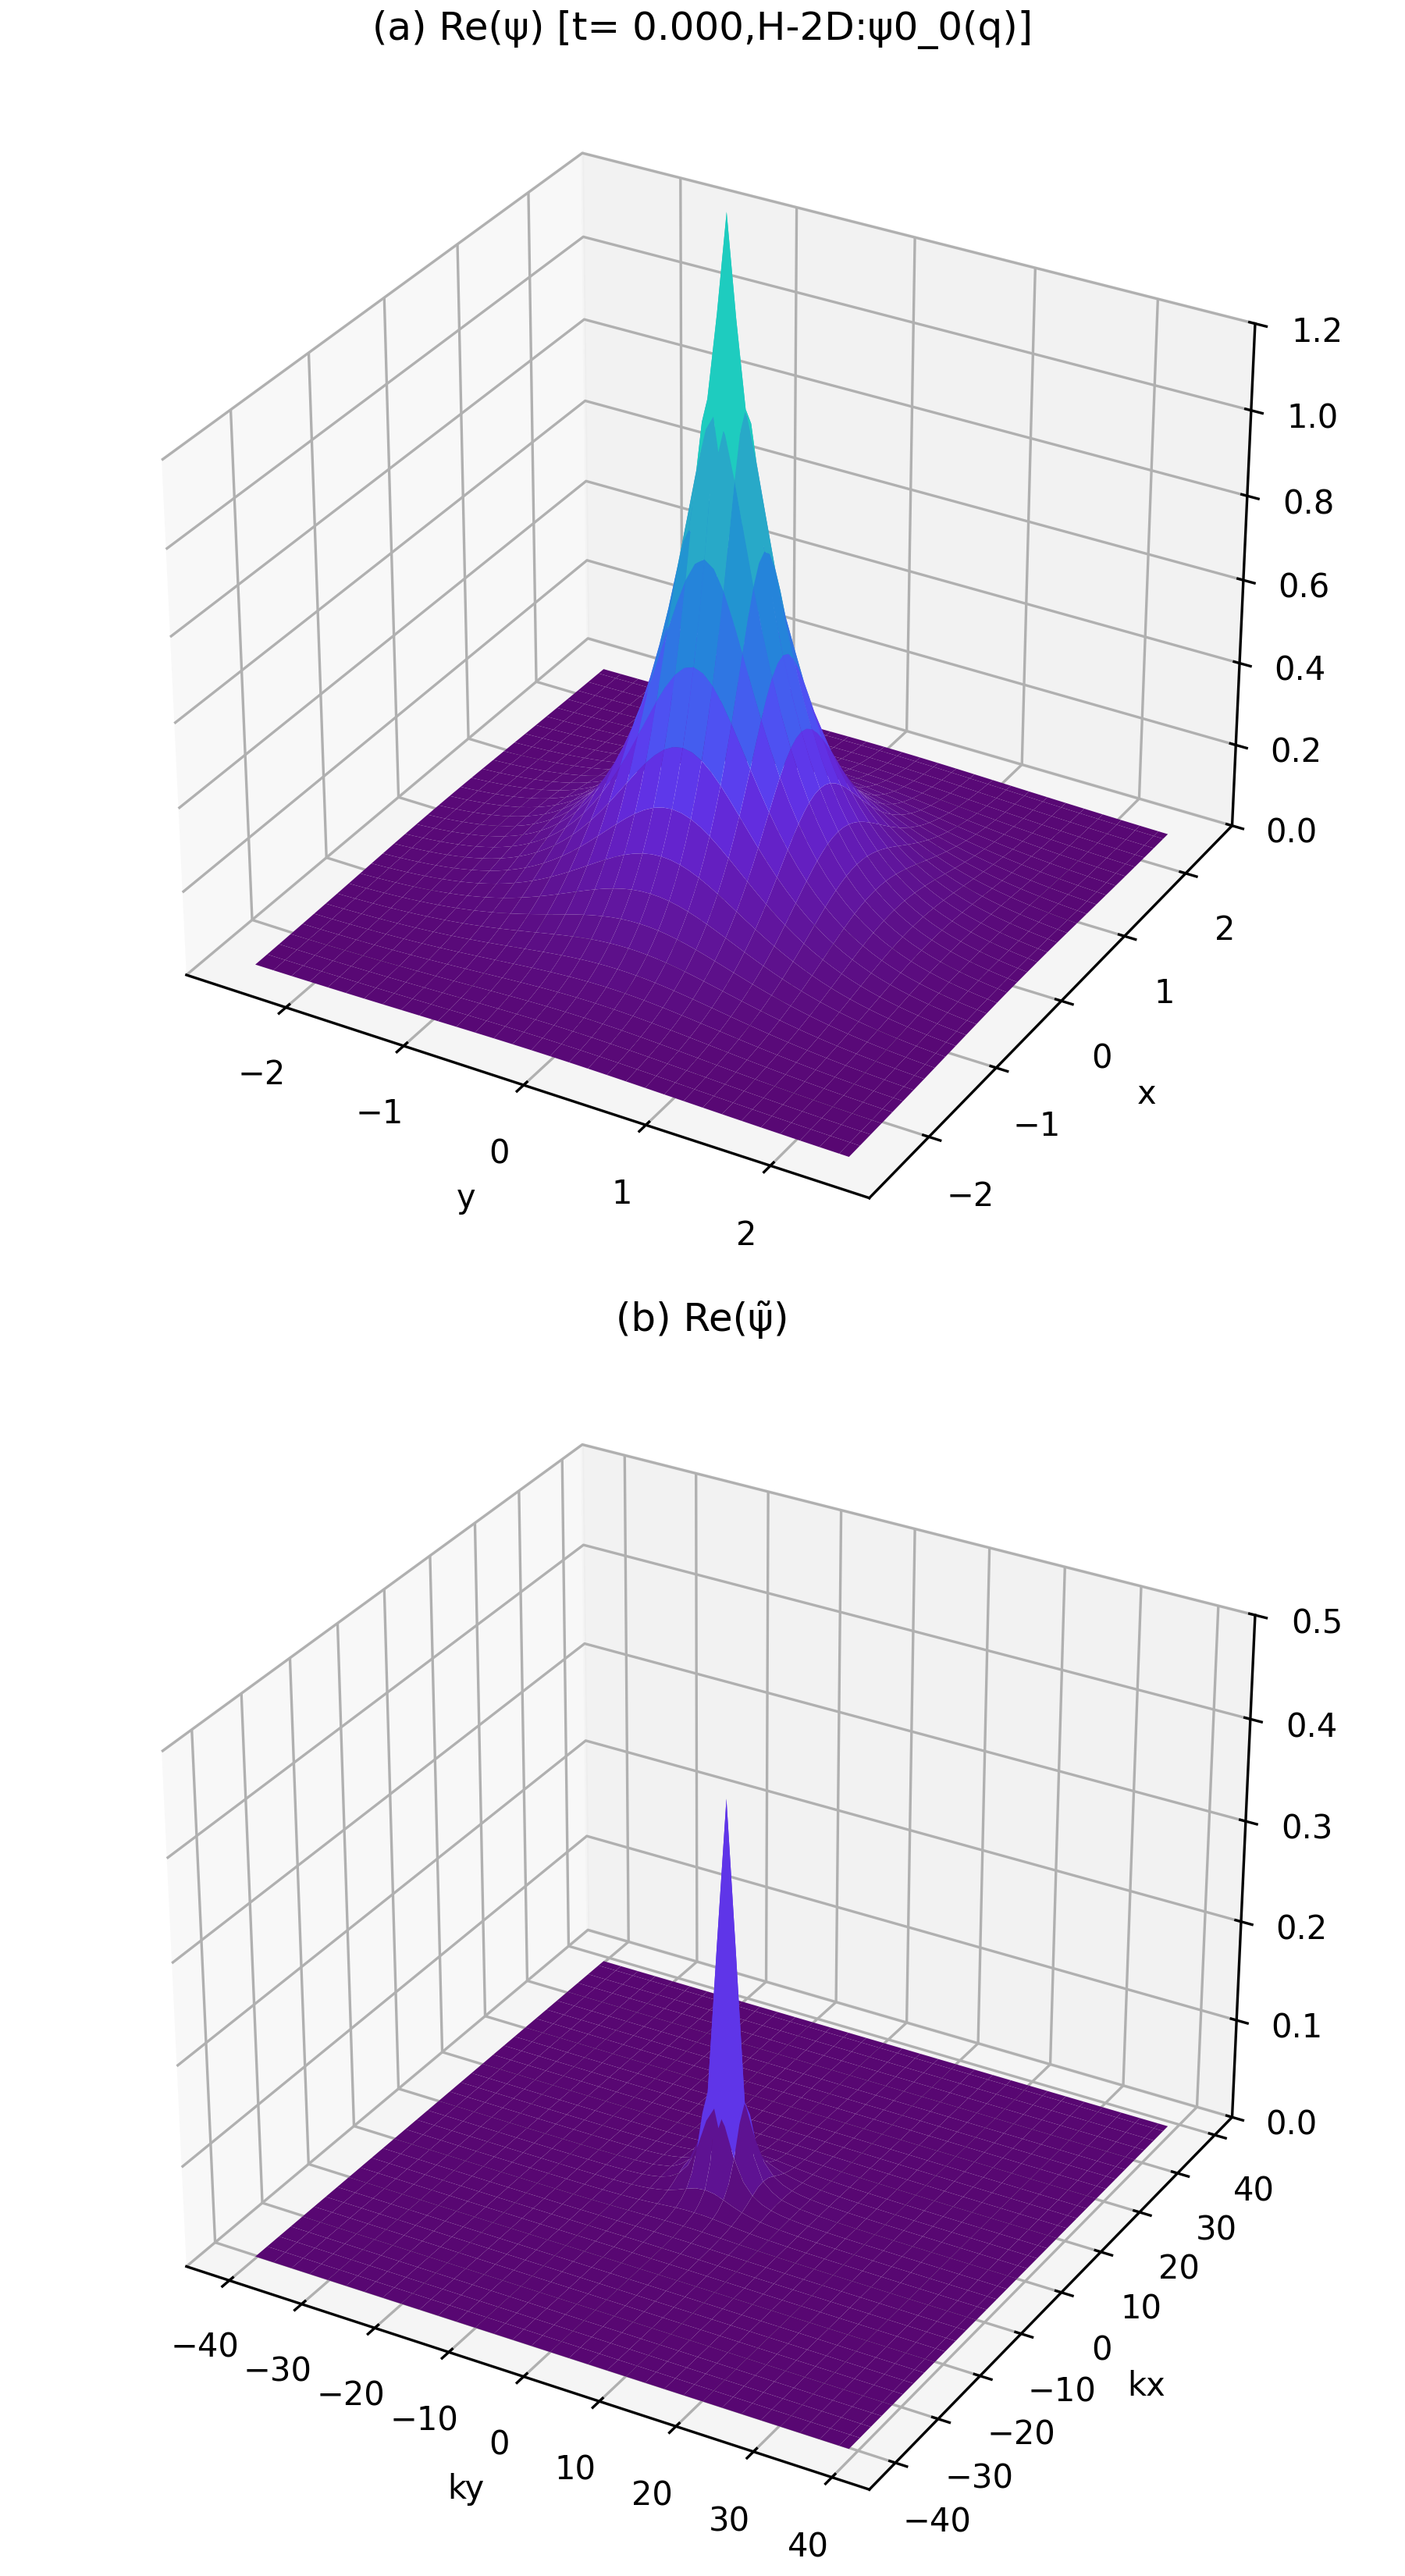
\includegraphics[width=1\columnwidth]{paper2025_figs/classic2D/6b_n0_m0/t_00.000_3d-qp.png}
        \caption{Wavefunction $\PsiTwoD_{0,0}$}
        \label{subfig:initial-wavefunction-2d-0-0}
    \end{subfigure}
    \begin{subfigure}{.45\columnwidth}
        \centering
        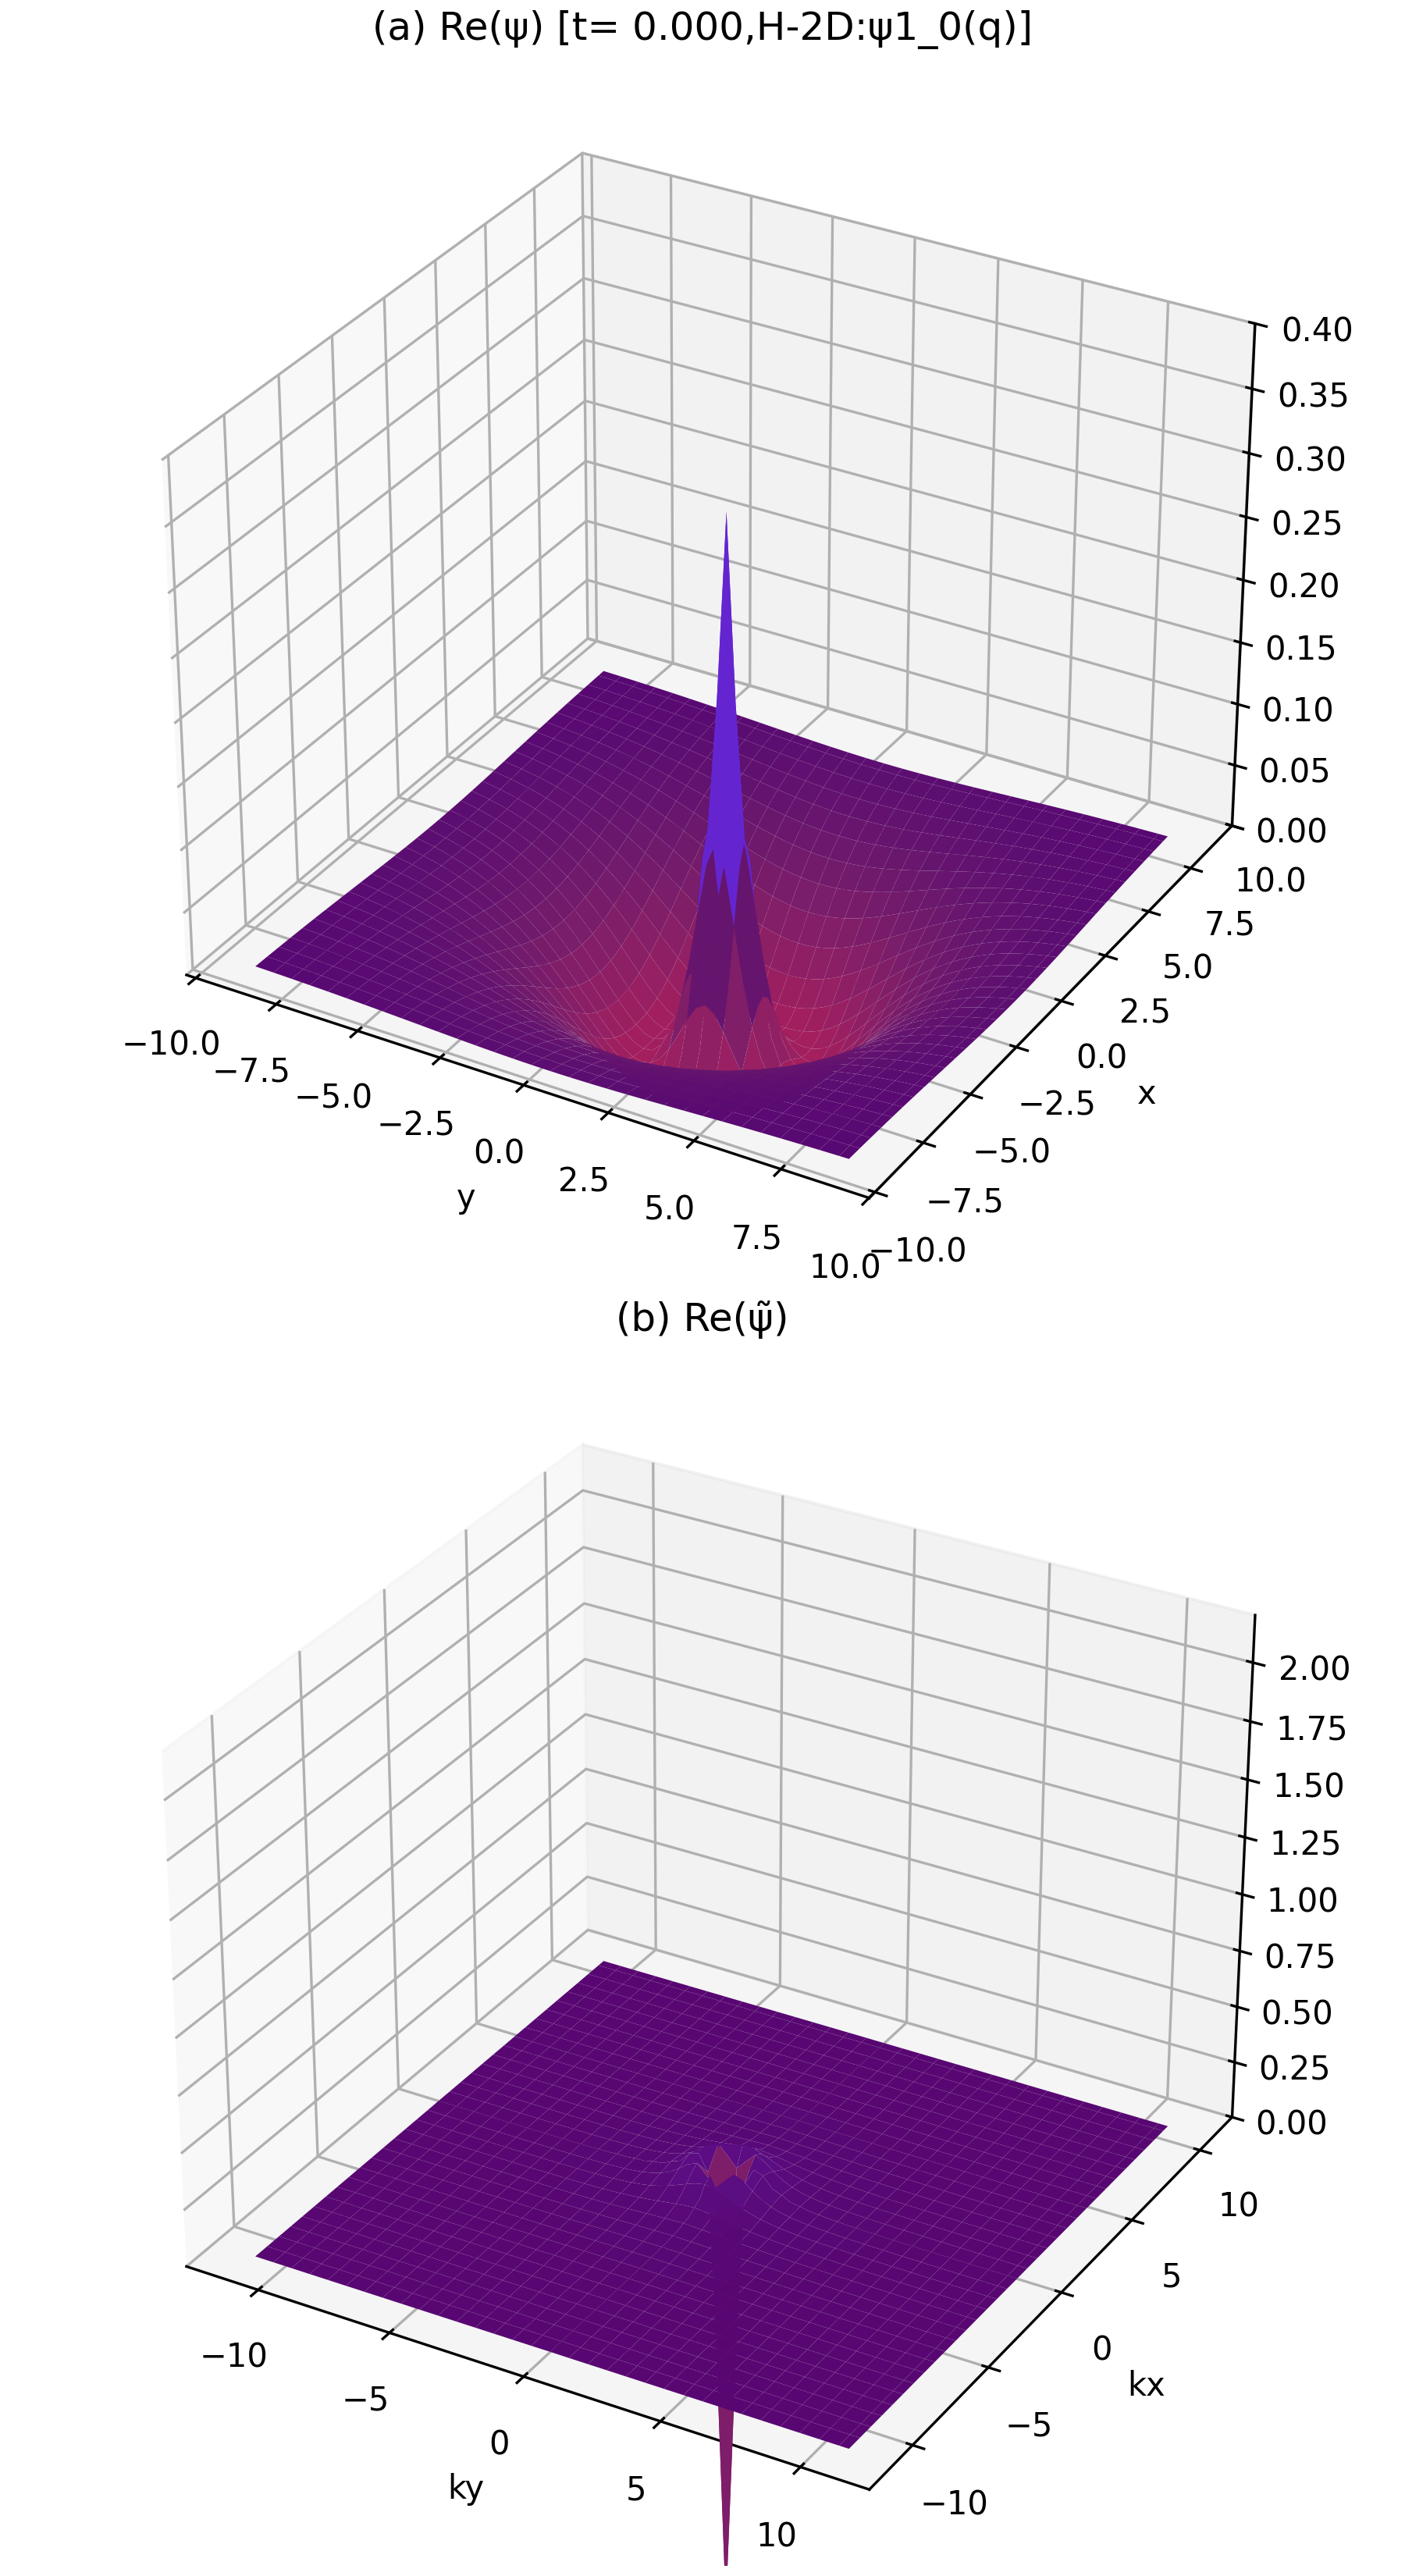
\includegraphics[width=1\columnwidth]{paper2025_figs/classic2D/6b_n1_m0/t_00.000_3d-qp.png}
        \caption{Wavefunction $\PsiTwoD_{1,0}$}
        \label{subfig:initial-wavefunction-2d-1-0}
    \end{subfigure}
    \begin{flushleft}\small 

        (a) Ground state $\PsiTwoD_{0,0}$ with principal quantum number $n=0$
        and azimuthal quantum number $m=0$
        (Eq. \ref{eq:psi2D00-wave-function}).
        (b) Excited state $\PsiTwoD_{1,0}$ with $n=1,m=0$
        (Eq. \eqref{eq:psi2D10-wave-function}).
        In each panel, the top row shows the real part in real space and the
        bottom row shows the real part in k-space. In both (a) and (b), the
        wavefunction value at the origin is nonzero.

    \end{flushleft}
\end{figure}

\begin{figure}[ht]
    \centering
    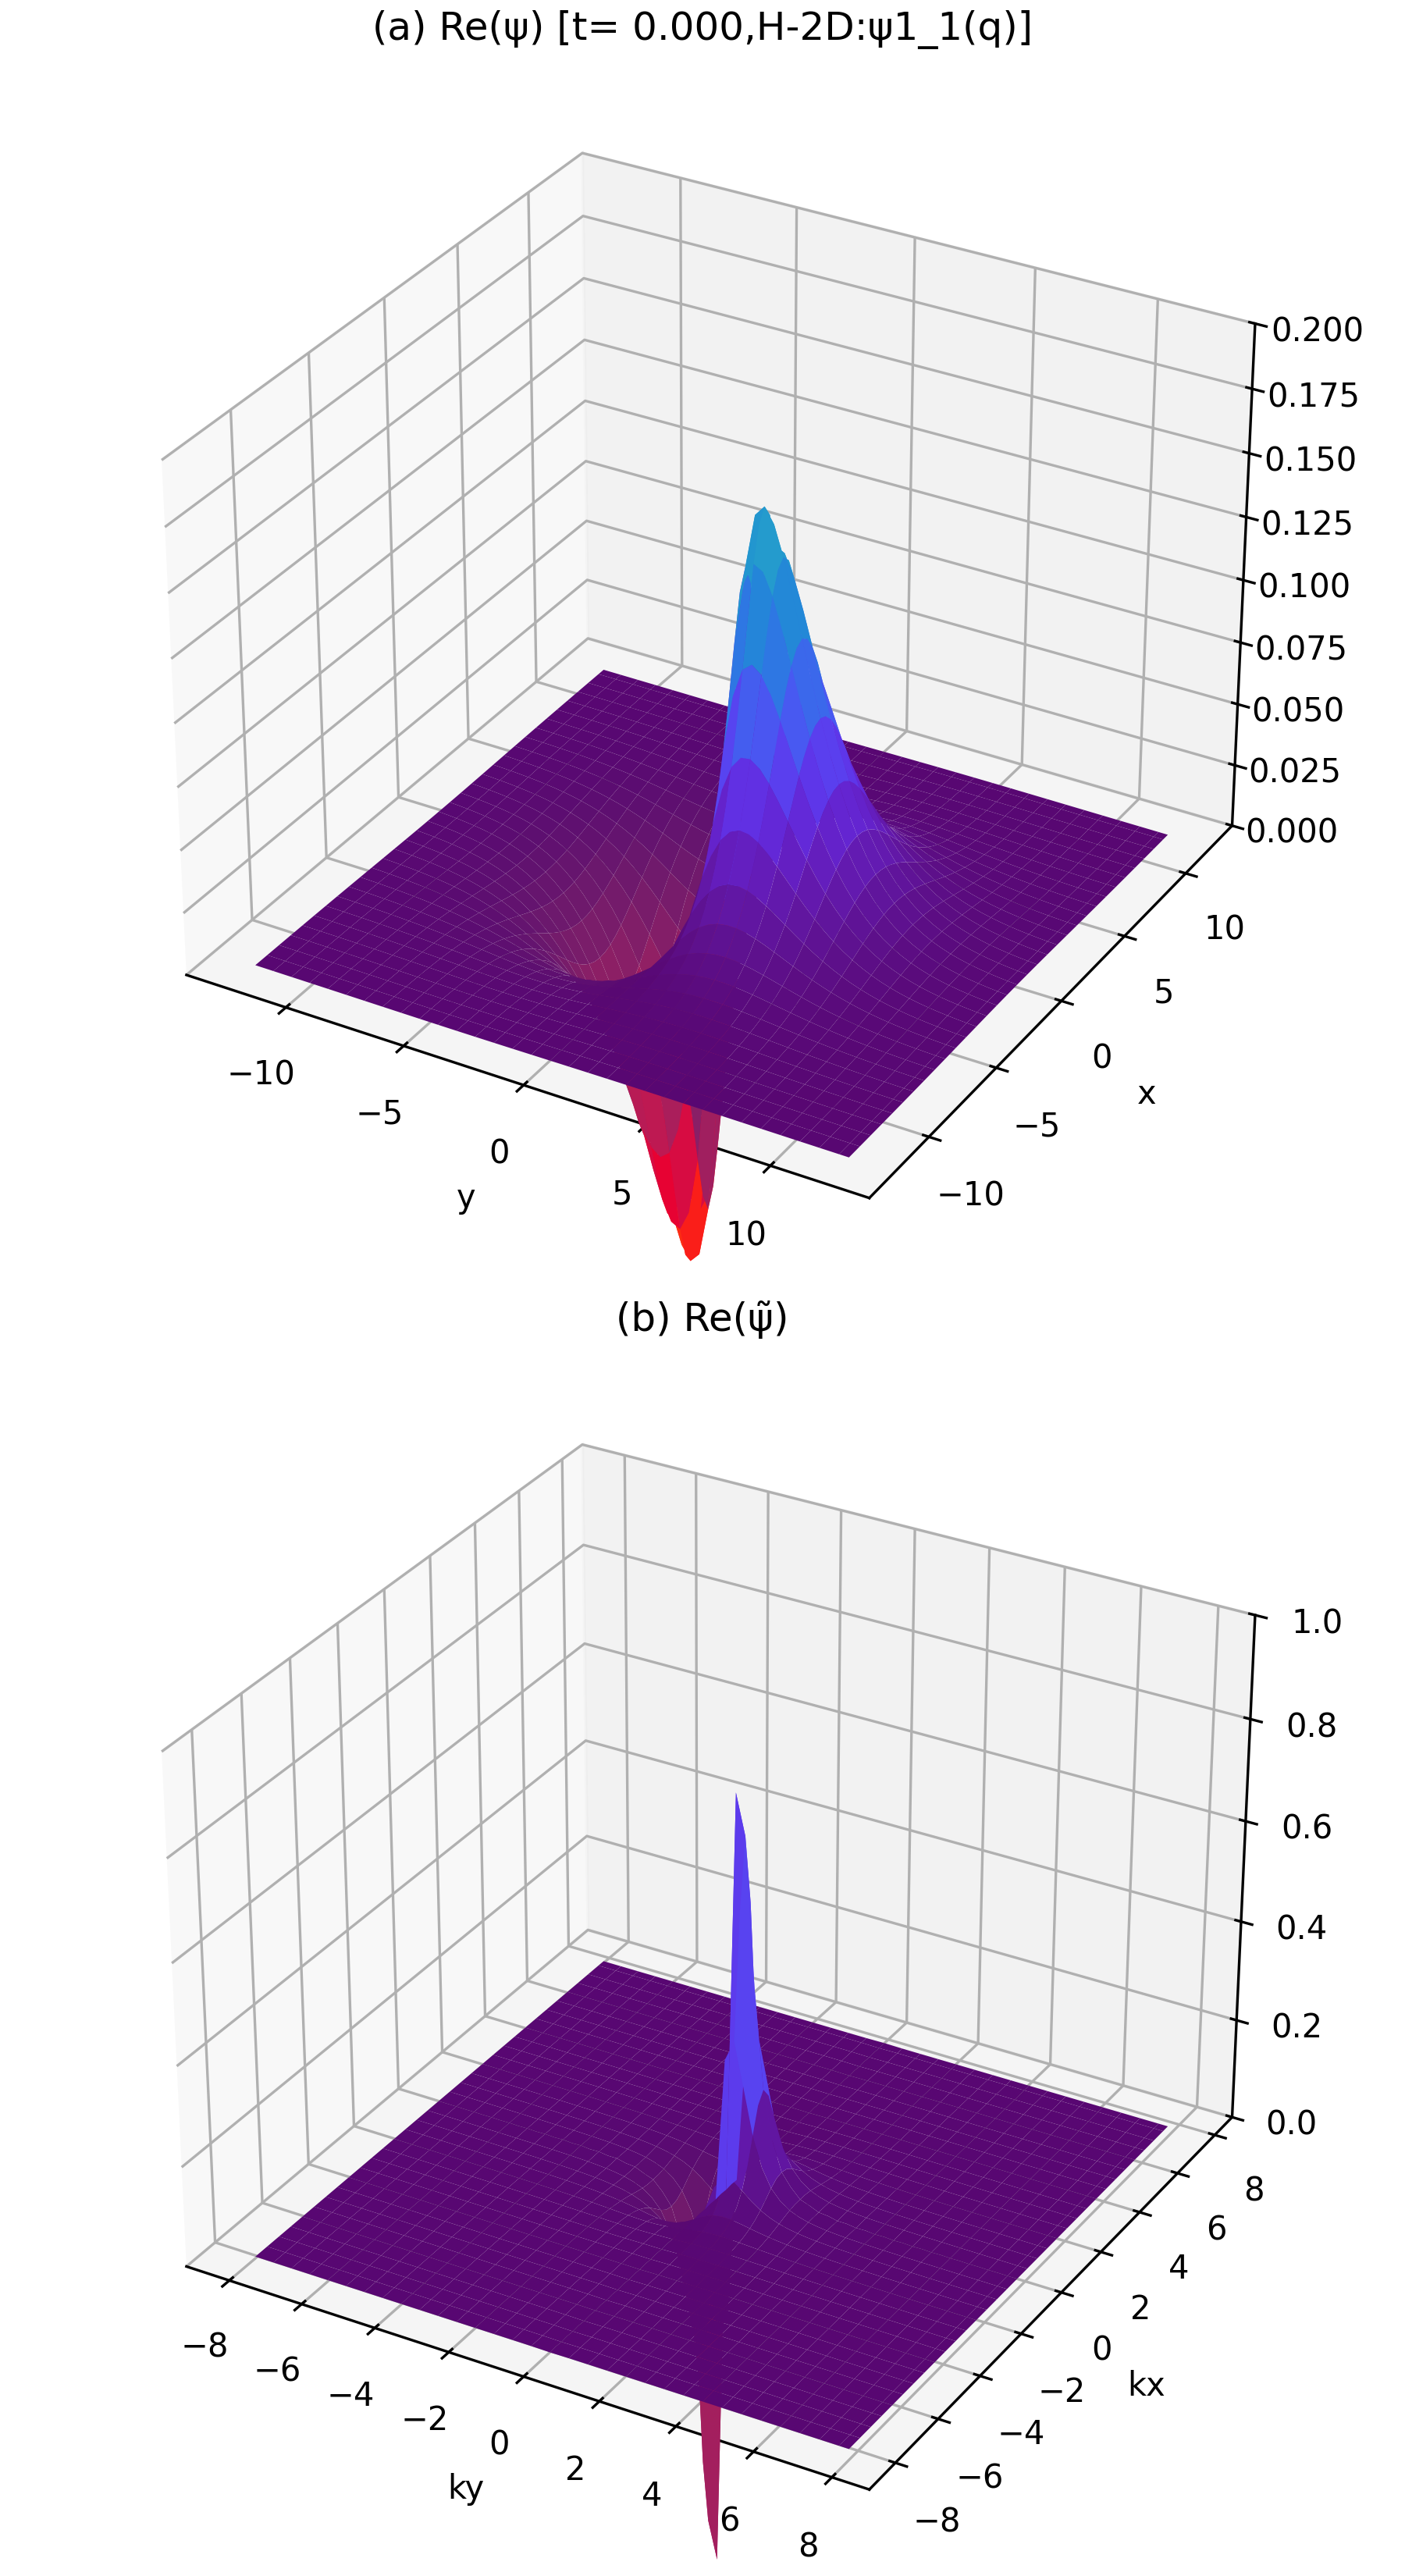
\includegraphics[width=0.45\columnwidth]{paper2025_figs/classic2D/6b_n1_m1/t_00.000_3d-qp.png}
    \caption{Wavefunction $\PsiTwoD_{1,1}$}
    \label{subfig:initial-wavefunction-2d-1-1}
    \begin{flushleft}\small

        Excited state $\PsiTwoD_{1,1}$ with $n=1,m=1$
        (Eq. \ref{eq:psi2D11-wave-function}).
        In each panel, the top row shows the real part in real space and the
        bottom row shows the real part in k-space. The wavefunction value at the
        origin is zero.

    \end{flushleft}
\end{figure}


\clearpage
\subsection{Use of an Auxiliary Classical Time-Evolution Simulator}
To run the simulator circuits of this study on a quantum-computer emulator, the
circuit qubit count and gate count must remain within emulator limits.
Accordingly, the range of model parameters that can be directly tested is
limited. To evaluate parameter values beyond emulator-executable ranges, we
also use a classical program constructed to be operationally equivalent to the
simulator circuit. Parameters actually executed on the simulator circuit are
listed in Table \ref{tab:emulator-circuit-configurations} in
Section \ref{subsec:circuit-size-evaluation}.

\subsection{Use of a Quantum-Computer Emulator}
In this study, we execute quantum circuits not on physical quantum hardware but
on a quantum-computer emulator running on a classical computer. This is a
software tool provided as part of a quantum-circuit SDK
\cite{website:qiskit-aer}。

A quantum-computer emulator stores qubit state-vector contents in classical
computer memory, and executes qubit operations by expanding them over each
superposed state.

There are several ways to represent qubit states. In the simplest state-vector
method, the state vector for $N$ qubits is stored in memory as an array with
$2^N$ elements.

When entanglement is weak and long-range entanglement between distant qubits is
minimal, the Matrix Product State (MPS) method is known to greatly compress
memory usage by representing qubits as a chain of matrices, and is also
available in Qiskit emulators \cite{Vidal2003.PhysRevLett.91.147902}. However,
in first quantization, all qubits except ancilla qubits are essentially
entangled, so effective data compression by MPS is not expected. Therefore, we
use the state-vector method in this study.

Emulators can also simulate noise models of physical quantum hardware. However,
because the algorithm in this study requires many operations, it is intended
for operation on noise-resilient fault-tolerant quantum computers (FTQCs).
Accordingly, circuit design here does not consider noisy operation. We run the
emulator as an ideal quantum computer with zero noise.


\subsection{Computing Environment}
The computer hardware and software used for simulation are as follows.
\begin{itemize}
    \item CPU:AMD Ryzen 9 7950X 16 Core × 1
    \item Memory: 128GB
    \item GPU: NVIDIA GeForce RTX 4090 × 1
    \item OS: Ubuntu 22.04.4 LTS
    \item Quantum SDK: Qiskit 1.4.0, qiskit-aer-gpu 0.15.1
    \item Quantum chemistry simulator software: Chemical Reaction Simulator Q (crsQ) \cite{website:crsq}
\end{itemize}


\section{Strategies for Potential Calculation Under Limited Qubit Counts}
In early-stage error-corrected quantum computing, available qubits are expected
to be severely limited because error correction requires a large amount of
redundancy. Even on currently available QC emulators running on classical
computers, usable qubit counts are also tightly constrained due to exponential
memory and computational requirements in the number of qubits.

In standard resource-estimation approaches for quantum-chemistry circuits, one
starts from a target molecular model size and allowable error, then estimates
the required qubit and gate counts. In contrast, this report starts from the
available qubit count and explores how to determine executable circuit
configurations under that constraint. For this purpose, we focus on concrete
resource scales in small models, including circuit constructions that are not
necessarily efficient for large-scale models.

The major contributor to simulator-circuit size is the Coulomb-potential
calculation circuit. In the basic Coulomb-potential circuit based on Trotter
decomposition, the simulation domain (a rectangular region) is divided into a
uniform grid; grid indices are mapped to multi-qubit registers; and the Coulomb
potential is computed by arithmetic operations on qubit values
\cite{Zalka-rspa.1998.0162}. Binary arithmetic circuits are used for these
operations \cite{Vedral1996.PhysRevA.54.147}. The resulting circuit scales
polynomially in both qubit and gate counts with respect to particle number,
which is exponentially better than classical computation.

This is the baseline computational method. However, although asymptotically
efficient, the constant factors in required ancilla qubits and gate counts are
not small.

A proposed gate-reduction approach first obtains an approximate value of
$1/\sqrt{x}$ by QROM, then approximates $1/\sqrt{x}$ with a cubic polynomial
and improves the precision using Newton-Raphson iteration
\cite{Rubin2024.pnas.2317772121}.

In this study, we additionally examine a method that reduces ancilla-qubit
count even if gate count increases.

In this section, we introduce the above three methods, and for the first and
third methods we implement and evaluate actual circuits.

\subsection{Potential-Calculation Circuit Using Arithmetic Gates}
\label{subsec:potential-circuit-by-arithmetic-gates}

The fundamental approach to Coulomb-potential calculation circuits is based on
arithmetic circuits
\cite{Zalka-rspa.1998.0162}。

\begin{figure}[ht]
    \centering
    \begin{quantikz}[transparent]
        \lstick{$n_1$} & \qwbundle{\nb} & \gate[4]{\Thetaep} &                   & \gate[4]{\Thetaep} &\\
        \lstick{$n_2$} & \qwbundle{\nb} &                    &\gate[3]{\Thetaep} & \linethrough &\\
        \lstick{$n_3$} & \qwbundle{\nb} & \linethrough       &                   & & \\
        \lstick{$tmp$} & \qwbundle{} &                    &                   & &
    \end{quantikz}

    \caption{Example Coulomb-potential-term circuit $\Thetaep$ in a three-electron system}
    \label{fig:theta-ep-multi-electron}
    \begin{flushleft}\small
        
        $n_1,n_2,n_3$ are registers corresponding to discretized coordinates of
        electrons 1, 2, and 3, respectively, each consisting of $\nb$ bits. A
        slashed qubit line indicates a multi-qubit register rather than a single
        qubit. $tmp$ is an ancilla-qubit register. The Coulomb-potential circuit
        $\Thetaep$ must be provided for each electron pair, i.e., (1,2), (2,3),
        and (1,3), but only one ancilla register set is needed. Qubit wires
        passing through a $\Thetaep$ box indicate qubits not used by that
        circuit.
    \end{flushleft}
\end{figure}

This circuit requires a substantial number of ancilla qubits to store
intermediate values. In systems with many particles, arithmetic circuits are
required for each particle pair, but one ancilla register set can be reused
across different pairs. Therefore, as shown in
Figure \ref{fig:theta-ep-multi-electron}, the ancilla-qubit count can remain
constant even when particle number increases. For this reason, ancilla count is
not usually emphasized when evaluating qubit-count scaling with particle number.
However, in small models, ancilla qubits can still occupy a significant
fraction of total circuit qubits.

Figure \ref{subfig:circuit-1d-arith-overall} shows the overall simulator circuit
using arithmetic circuits. The simulator consists of a state-preparation
circuit and a time-evolution circuit. The time-evolution circuit dominates the
qubit count.

Figure \ref{subfig:circuit-1d-arith-time-evolution} shows the internal structure
of the time-evolution circuit $\Thetae$ (Eq. \eqref{eq:circuit-eval-theta-e}).
The time-evolution circuit consists of a Coulomb-potential-energy-term circuit
$\Thetaep$, an inverse QFT circuit, a kinetic-energy-term circuit $\Thetaek$,
and a QFT circuit. Figure \ref{subfig:potential-energy-circuit-1d-arith} shows
$\Thetaep$, which computes $1/|x|$.

\begin{figure}[ht]
    \centering
    \begin{subcaptionblock}[T][][t]{0.3\columnwidth}
        \centering
        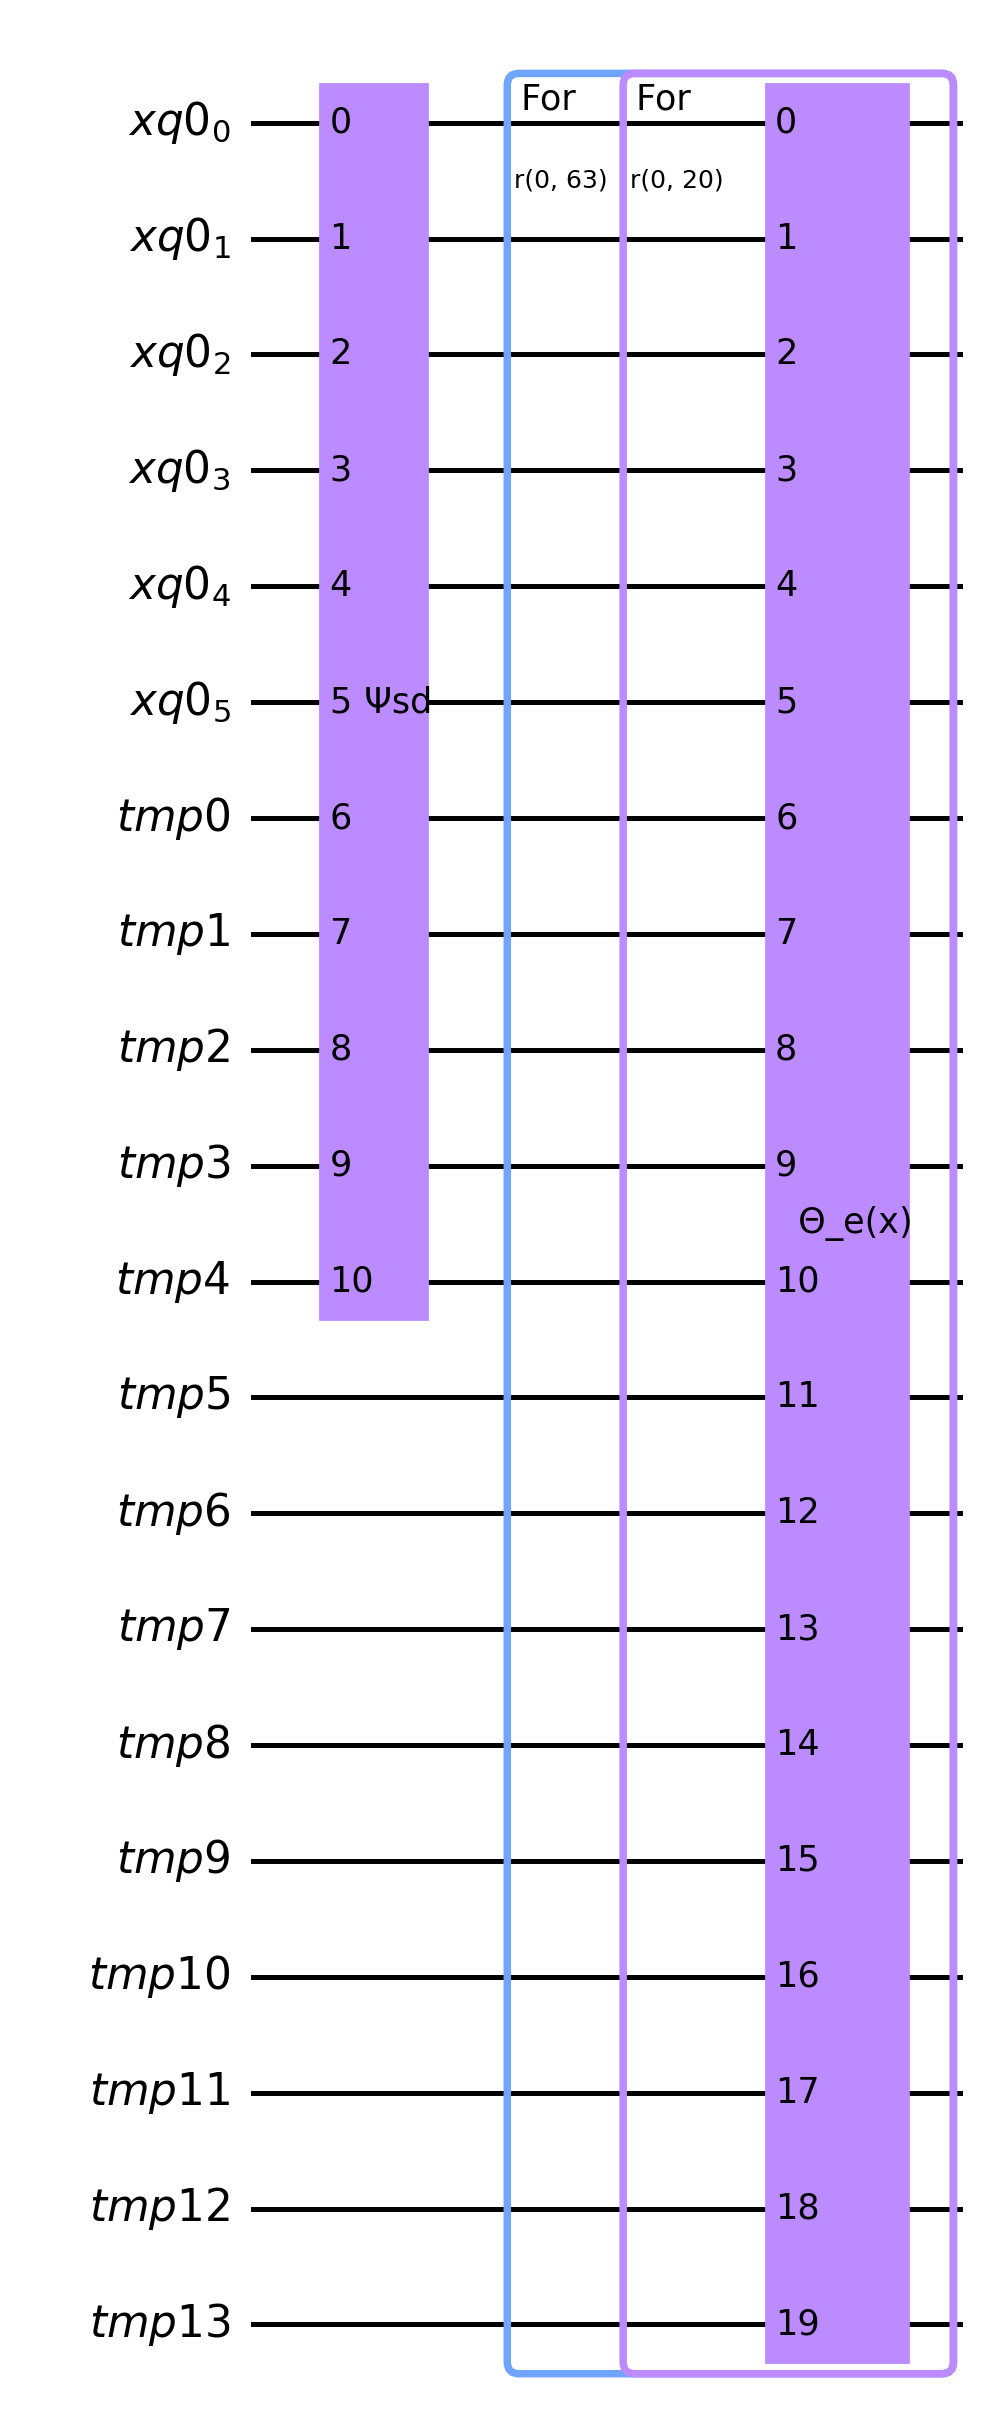
\includegraphics[width=\textwidth]{paper2025_figs/arith1D/circuit.png}
        \caption{Overall circuit}
        \label{subfig:circuit-1d-arith-overall}
    \end{subcaptionblock}
    \begin{subcaptionblock}[T][][t]{0.42\columnwidth}
        \centering
        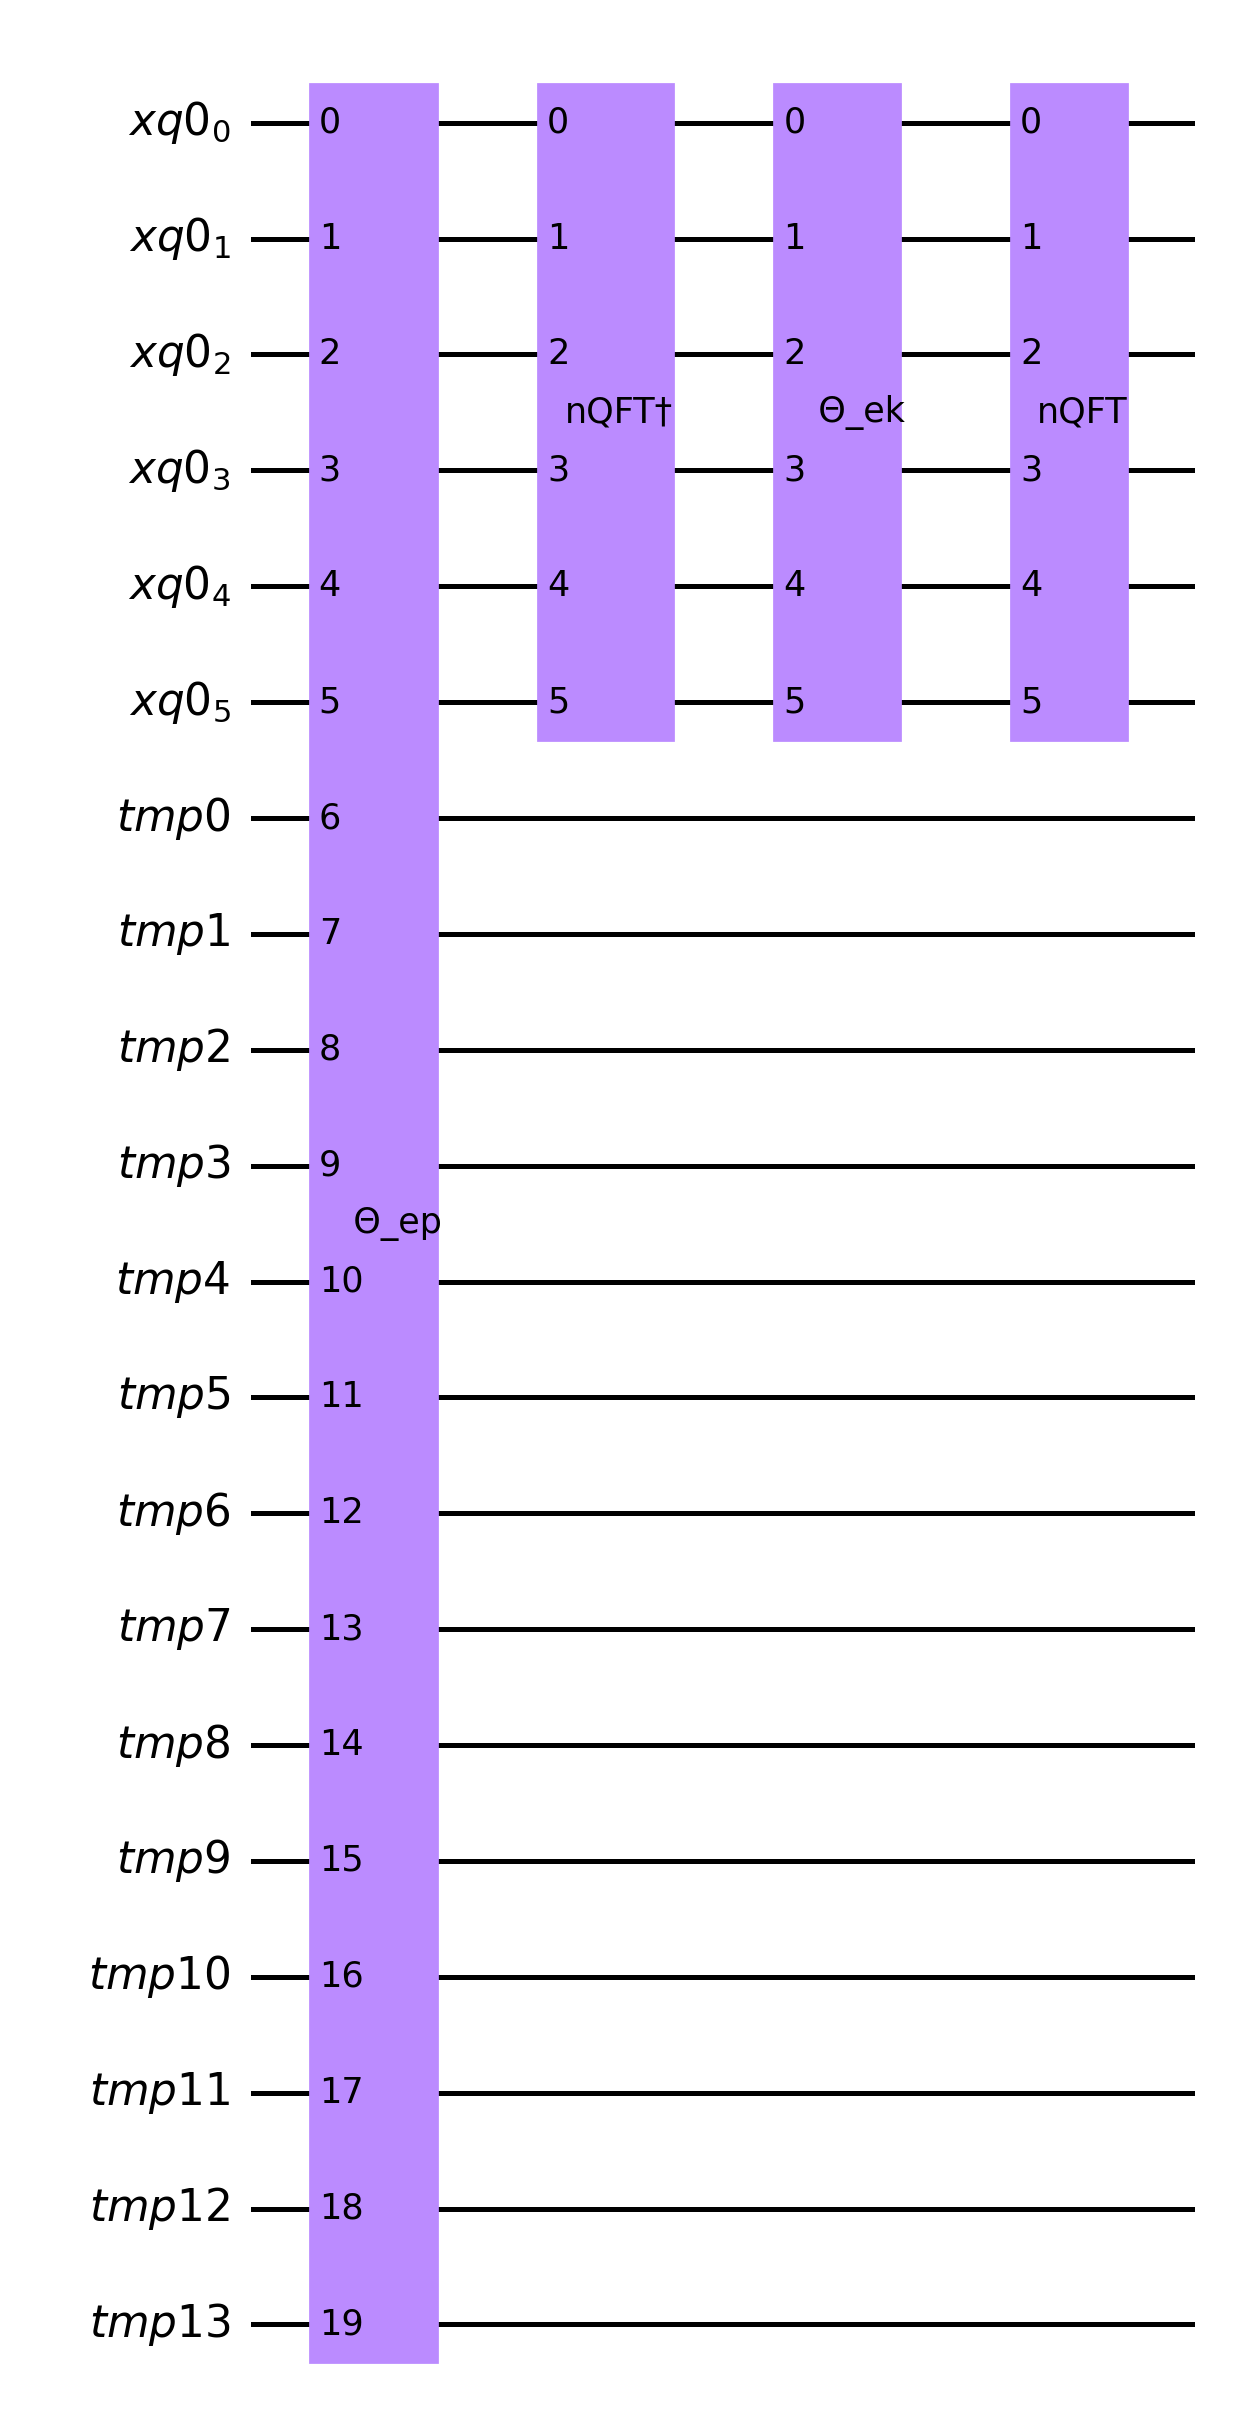
\includegraphics[width=\textwidth]{paper2025_figs/arith1D/elec_motion.png}
        \caption{Internal structure of time-evolution circuit $\Thetae$}
        \label{subfig:circuit-1d-arith-time-evolution}
    \end{subcaptionblock}
    \caption{Simulator circuit for the one-dimensional model using arithmetic gates}
    \label{fig:circuit-1d-arith}
    \begin{flushleft}\small

        (a) Overall simulator circuit for the one-dimensional model. The circuit
        consists of initialization circuit $\PsiSD$ and time-evolution circuit
        $\Thetae$. (b) Internal configuration of $\Thetae$, composed of
        potential-energy-term circuit $\Thetaep$, inverse QFT, kinetic-energy-
        term circuit $\Thetaek$, and QFT. The 23-qubit size of $\Thetaep$
        determines the total circuit qubit count.

    \end{flushleft}
\end{figure}

\begin{figure}[ht]
    \centering
    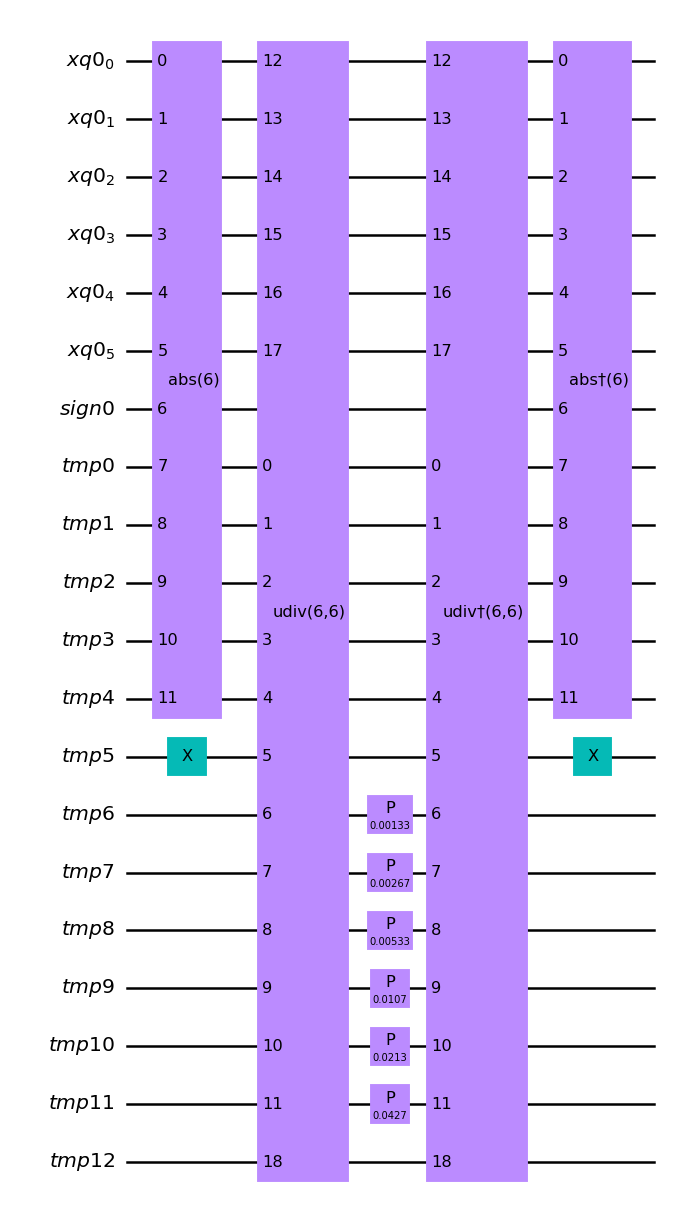
\includegraphics[width=0.5\textwidth]{paper2025_figs/arith1D/elec_potential_arithmetic.png}
    \caption{Potential-energy-term circuit $\Thetaep$ using arithmetic gates}
    \label{subfig:potential-energy-circuit-1d-arith}
    \begin{flushleft}\small

        Internal structure of Coulomb-potential-term circuit $\Thetaep$
        implemented with arithmetic gates. The value $1/|x|$ is computed in
        binary, and phase is shifted with P gates according to the bit weights
        of the result. The qubit count of division gate `udiv7` is dominant. The
        total ancilla-qubit count is 17 bits.

    \end{flushleft}
\end{figure}
\clearpage
\subsection{Potential-Calculation Circuit Combining QROM and Newton-Raphson}
\label{subsec:potential-circuit-by-qrom-newton-raphson}

In prior studies of first-quantized time-evolution simulation, constant factors
in qubit count are often accepted while reducing gate count is actively pursued.
For example, one improvement avoids both costly square-root and division
operations by obtaining an initial estimate with Quantum Read Only Memory
(QROM), then refining it with one Newton-Raphson step
\cite{Rubin2024.pnas.2317772121}. In this method, $1/\sqrt{x}$ is approximated
by a cubic polynomial and solved via Newton-Raphson. To increase accuracy, the
domain is partitioned and polynomial coefficients are changed per segment. To
limit Newton-Raphson to a single step, an approximate $1/\sqrt{x}$ value is
provided by QROM. In the original QROM proposal, QROM circuits require gate
count exponential in input bits \cite{Babbush_2018b.PhysRevX.8.041015}. Here,
the Variable Spacing method proposed in
\cite{Sanders2020.PRXQuantum.1.020312} reduces the QROM gate count to the order
of bit count.

This method can reduce gate count by avoiding square-root and division circuits,
but the ancilla-qubit count required by QROM remains large, because QROM
requires ancilla qubits proportional to output bit count. Therefore, in small
models, ancilla qubits occupy a large fraction of total qubits and do not help
reduce overall circuit qubit count. The method is effective mainly for larger
models with sufficiently many particles.

Because this approach requires many qubits and is difficult to run on an
emulator, we do not implement it in this study.

\subsection{Potential-Calculation Circuit Using UCRZ Gates}
\label{subsec:potential-circuit-by-ucrz-qubits}

In this study, because we treat simulations of models with few electrons, we
also consider constant-size ancilla counts important, and focus on Uniformly
Controlled Rotation (UCR) circuits, whose behavior is similar to QROM, as a
means of reducing ancilla qubits
\cite{Mottonen2004.PhysRevLett.93.130502}.
In one variation, the UCRZ circuit outputs a phase-rotation angle on a target
qubit. This has the same output form as the Coulomb-potential circuit, so the
UCRZ output can be used directly as the Coulomb-potential-circuit output. UCRZ
requires only one target ancilla qubit, enabling a substantial ancilla
reduction relative to arithmetic circuits. However, like QROM, its gate count
is exponential in control-register size, making it impractical for large
models, while still effective for small models. UCRZ is useful as an
alternative when total qubit count is limited. In this study, using UCRZ makes
two-dimensional model calculations executable on the emulator.

A UCR circuit applies a rotation around a specific axis $a$ to a single target
qubit $t$ according to the bit pattern of an $n$-bit input register
\cite{Mottonen2004.PhysRevLett.93.130502}.
Given that it outputs preassigned values for each input, UCR can be regarded as
a type of QROM circuit. Unlike general QROM, which outputs a bit string on an
output register, UCR outputs a rotation angle on the target qubit. Since UCRZ
outputs target-qubit phase shifts, it can be directly used for the potential
term of the time-evolution operator, replacing both interparticle-distance and
reciprocal calculations with a single UCRZ circuit. As a result, many ancilla
qubits required by arithmetic circuits can be eliminated.

The action of the UCR circuit is expressed as
\begin{equation}
    \ket{b}\ket{t} \mapsto \ket{b} R_{\mathrm{a}}(\theta_{\mathrm{b}})\ket{t}
\end{equation}
holds.

\begin{figure}[ht]
    \centering
    \begin{quantikz}[column sep=0.3cm]
        \lstick{$b_0$} & & \ctrl{3} & &          & & \ctrl{3} & &          & & \ctrl{3} & &          & & \ctrl{3} & &          &\\
        \lstick{$b_1$} & &          & & \ctrl{2} & &          & &          & &          & & \ctrl{2} & &          & &          &\\
        \lstick{$b_2$} & &          & &          & &          & & \ctrl{1} & &          & &          & &          & & \ctrl{1} &\\
        \lstick{$t$} & \gate{\mathrm{R_0}} & \targ{} & \gate{\mathrm{R_1}} & \targ{} & \gate{\mathrm{R_2}} & \targ{} & \gate{\mathrm{R_3}} & \targ{} &
                       \gate{\mathrm{R_4}} & \targ{} & \gate{\mathrm{R_5}} & \targ{} & \gate{\mathrm{R_6}} & \targ{} & \gate{\mathrm{R_7}} & \targ{} &
    \end{quantikz}
    \caption{Example UCRZ circuit with 3-bit input}
    \label{fig:ucrz-n3}
    \begin{flushleft}\small For the 3-bit input register $b_2b_1b_0$, there are
    8 possible input values, and the corresponding 8 Rz gates act on the target
    qubit. $\mathrm{R}_k$ denotes $\mathrm{Rz}(\theta_k)$. Each Rz gate applies a
    phase rotation by a preassigned angle $\theta_k$. C-NOT gates are placed
    before and after Rz gates so that the action of Rz gates is inverted
    depending on the input-register bit pattern.
    \end{flushleft}
\end{figure}

An $n$-bit-input UCRZ circuit consists of $2^n$ alternating C-NOT and Rz gates
acting on the target qubit. Figure \ref{fig:ucrz-n3} shows an example with
3-bit input.

The $k$-th Rz gate, $\mathrm{R_Z}_k$, rotates the phase by a preassigned angle
$\theta_k$. If no C-NOT inversion occurs, the total circuit rotation angle is
the sum of $\theta_k$. If inverted C-NOTs are present, all Rz gates between
inverted C-NOTs undergo sign inversion of rotation angle due to
$\mathrm{XR_z}(\theta)\mathrm{X}=\mathrm{R_z}(-\theta)$. In matrix form,
\begin{equation}
    \mathrm{XRz}(\theta)\mathrm{X} = \begin{pmatrix}
        0 & 1 \\
        1 & 0
    \end{pmatrix}
    \begin{pmatrix}
        e^{-i\theta/2} & 0 \\
        0 & e^{i\theta/2}
    \end{pmatrix}
    \begin{pmatrix}
        0 & 1 \\
        1 & 0
    \end{pmatrix}
    = \begin{pmatrix}
        e^{i\theta/2} & 0 \\
        0 & e^{-i\theta/2}
    \end{pmatrix}
    = \mathrm{Rz}(-\theta)
\end{equation}
which yields

Because each C-NOT control bit is connected to one bit of input register $b$,
the set of Rz gates whose action is inverted depends on $b$. As a result, the
total output rotation angle for input $b$ is
$\alpha_b=\sum_{k}{(-1)^{f_k(b)}\theta_k}$. That is, it is the sum of
$\theta_k$ with signs determined by $k$ and $b$. Since the inverse mapping from
$\theta_k$ to $\alpha_b$ is known, $\theta_k$ can be set so that desired
$\alpha_b$ is obtained for each input $b$.

In a Coulomb-potential-term circuit, particle-coordinate qubits are mapped to
grid points $\bm{\chi}_b$ indexed by UCR input value $b$, and the target-qubit
phase rotation angle $\alpha_b$ is set from the potential energy
$\Hp(\bm{\chi}_b)$ at that grid point as
\begin{equation}
\alpha_b = -\frac{\Hp(\bm{\chi}_b)\deltat}{\hbar}
\end{equation}
which yields the desired potential-energy-term circuit of the time-evolution
operator.

Figure \ref{fig:circuit-2d-ucrz} shows the simulator circuit using a UCRZ
circuit for the two-dimensional hydrogen model.

\begin{figure}[ht]
    \centering
    \begin{subcaptionblock}[T][][t]{0.3\columnwidth}
        \centering
        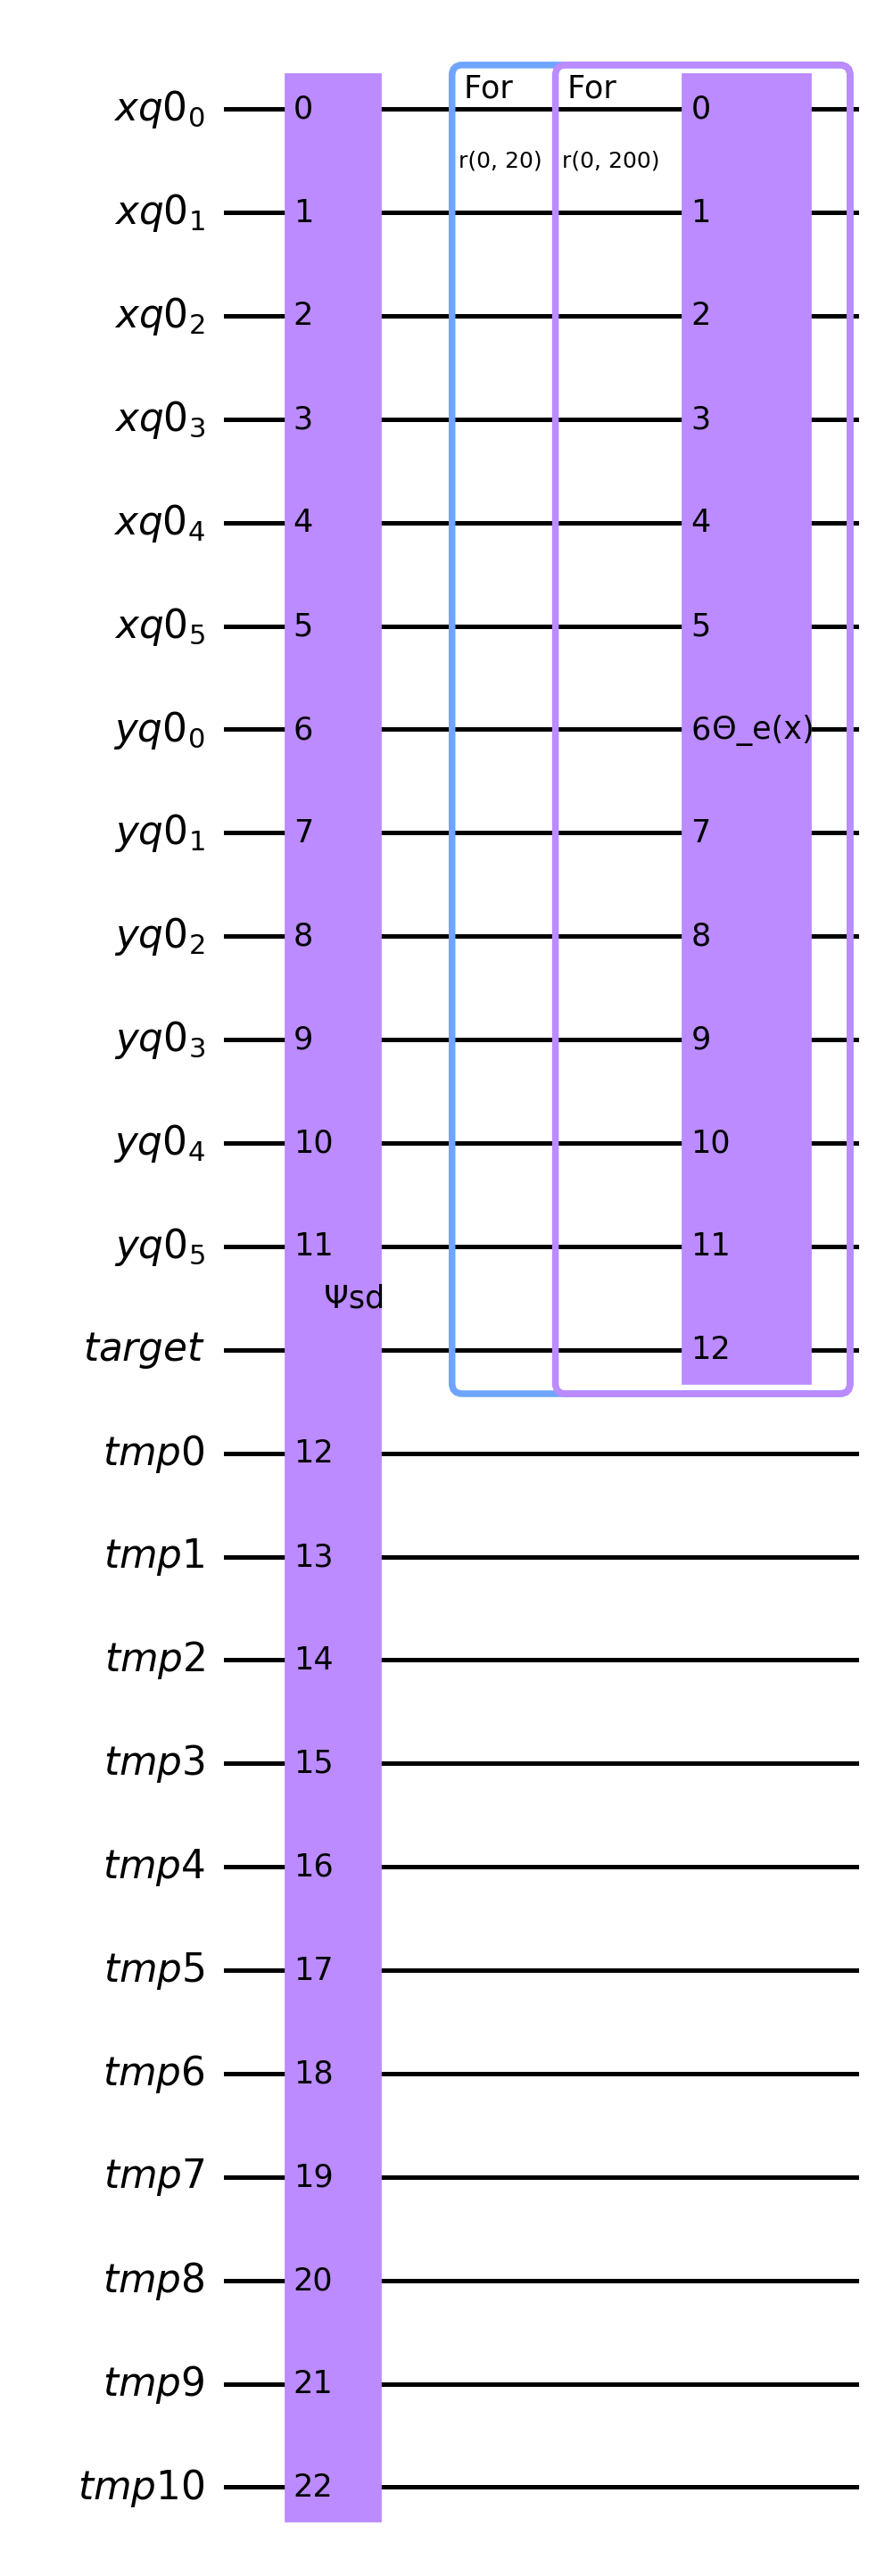
\includegraphics[width=\textwidth]{paper2025_figs/ucrz2D/circuit.png}
        \caption{Overall simulator}
        \label{subfig:circuit-2d-ucrz-overall}
    \end{subcaptionblock}
    \begin{subcaptionblock}[T][][t]{0.52\columnwidth}
        \centering
        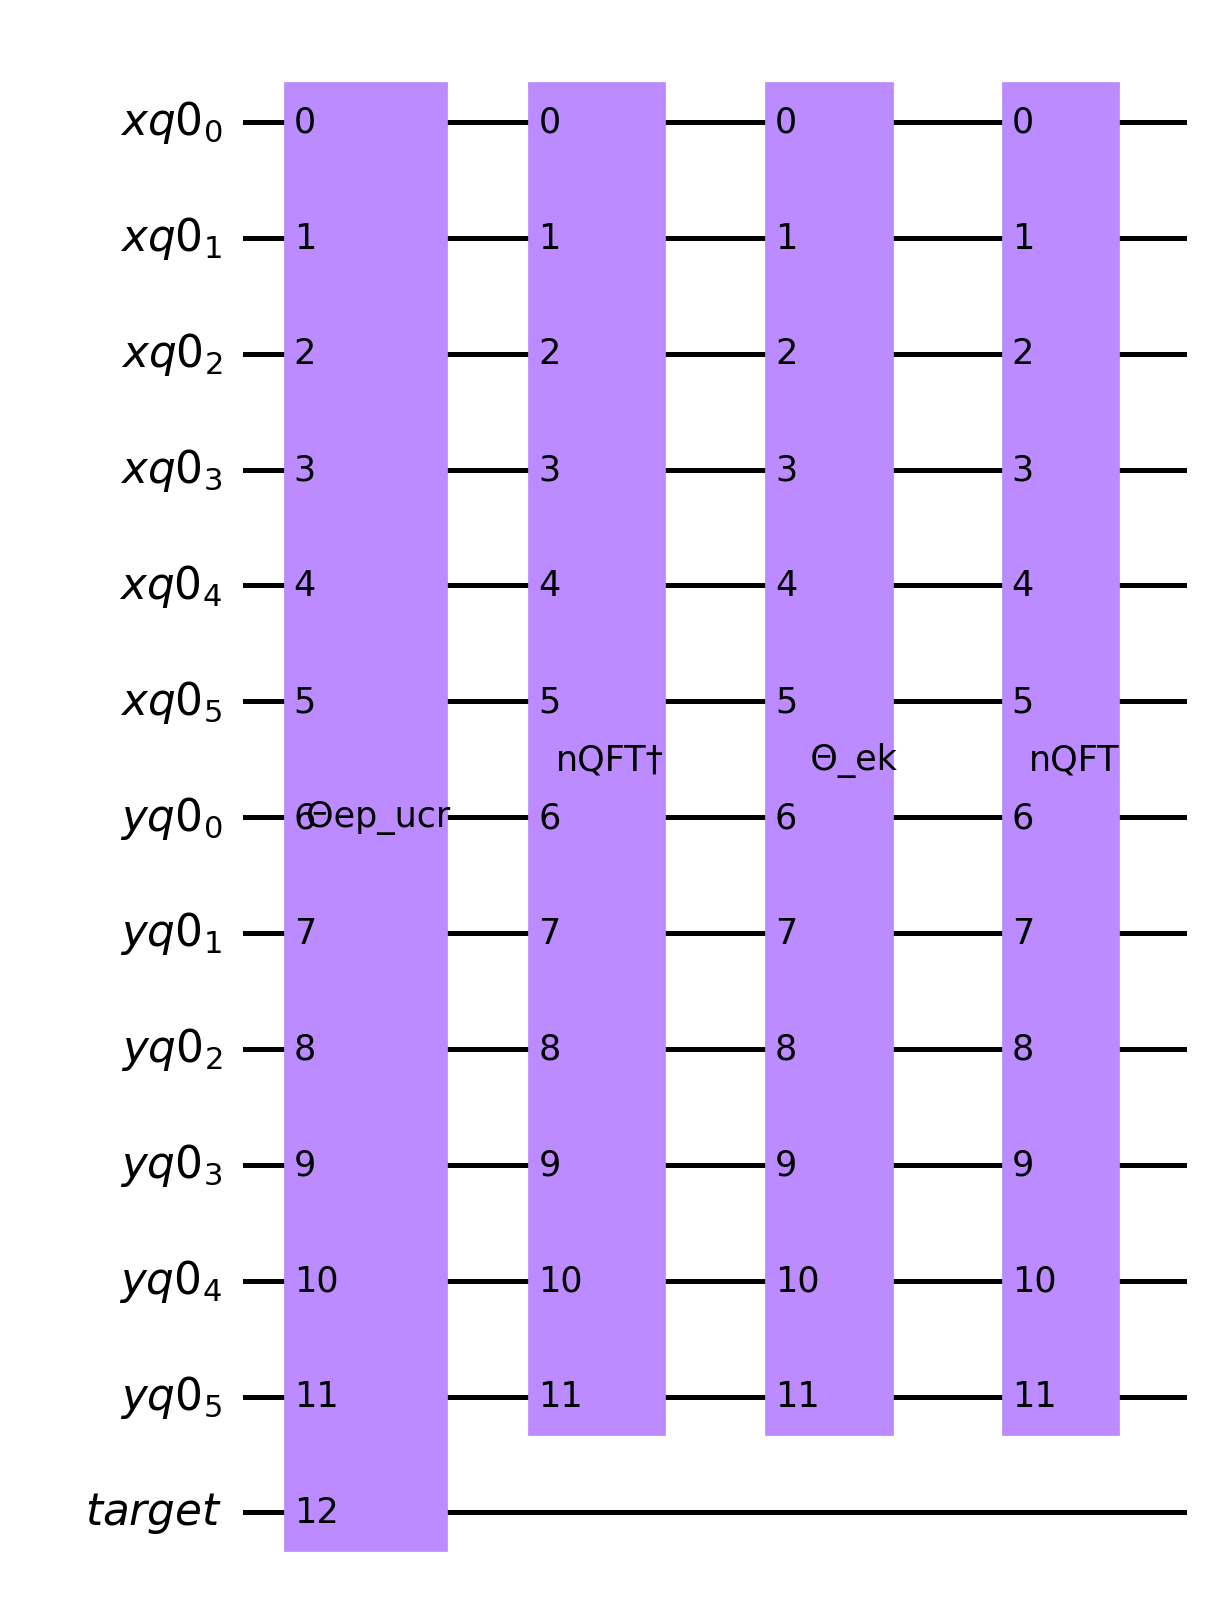
\includegraphics[width=0.8\textwidth]{paper2025_figs/ucrz2D/elec_motion.png}
        \caption{Internal structure of time-evolution circuit $\Thetae$}
        \label{subfig:time-evolution-circuit-2d-ucrz}
    \end{subcaptionblock}
    \caption{Simulator circuit for a two-dimensional model with 6-bit coordinate resolution using a UCRZ circuit}
    \label{fig:circuit-2d-ucrz}
    \begin{flushleft}\small

        (a) Overall simulator circuit, composed of a state-preparation circuit
        and a time-evolution circuit. The state-preparation circuit uses more
        qubits. (B) Configuration of the time-evolution circuit, where the
        potential-energy-term circuit $\Thetaepucr$ uses a UCRZ circuit, a type
        of Uniformly Controlled Rotation (UCR) circuit. In this example, for
        each superposed input value on the combined 12-bit input registers
        $xq0$, $yq0$ (6 bits each), the phase of ancilla qubit $target$ is
        adjusted accordingly. Only one ancilla qubit, $target$, is required.
    \end{flushleft}
\end{figure}

\clearpage
\subsection{Circuit-Size Evaluation}
\label{subsec:circuit-size-evaluation}
On the emulator in the computing environment used here, the maximum executable
qubit count was 27, and a practical upper bound on gate count was about $10^7$.
By generating simulator circuits and measuring their sizes, we examined circuit
configurations whose resource demands fall within this range.

\begin{figure}[ht]
    \centering
    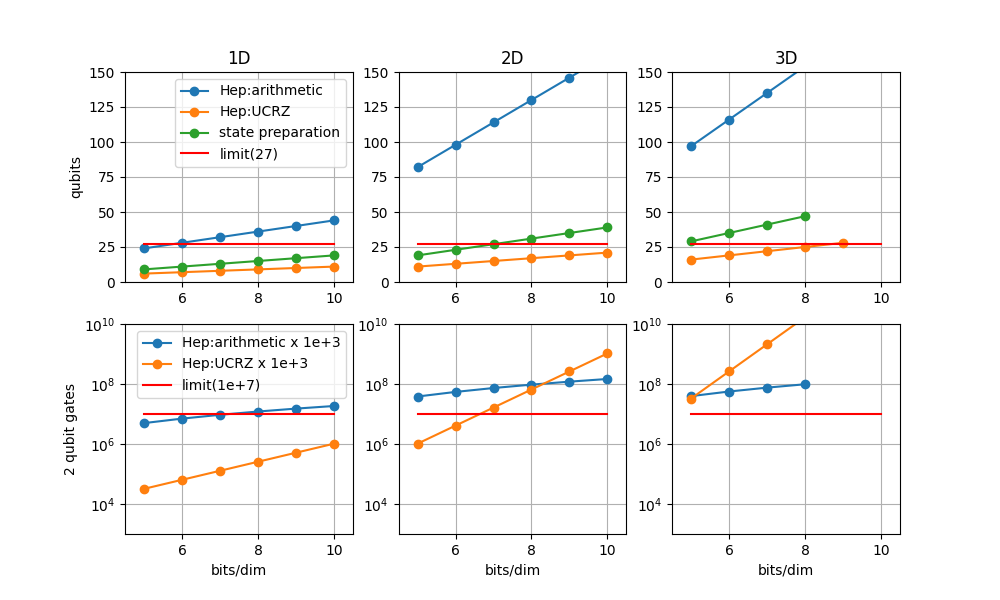
\includegraphics[width=15cm]{paper2025_figs/hamiltonian-gatecount.png}
    \caption{Circuit size}
    \label{fig:hamiltonian-gatecount}
    \begin{flushleft}\small
    The upper graphs show circuit qubit counts for 1D to 3D models. In
    descending order of qubit count, they show arithmetic-gate circuits, UCRZ
    circuits, and state-preparation circuits. Both state-preparation and
    time-evolution circuits must satisfy the qubit-limit constraint. Arithmetic
    circuits fit under the qubit limit only up to 7 bits in 1D. The
    state-preparation circuit fits up to the 2D 7-bit case. UCRZ circuits remain
    within range up to the 3D 8-bit case. The arithmetic-gate circuit qubit
    count differs greatly between 1D and 2D/3D because in 1D distance
    calculation needs only an absolute-value circuit, whereas 2D/3D require norm
    calculation with squaring and square-root circuits, making the circuit more
    complex.

    The lower graphs show numbers of two-qubit gates used by each circuit. For
    time-evolution circuits, gate counts are shown for 1000 steps as an example.
    State-preparation circuits are ignored because they are executed only once.
    Arithmetic-circuit gate counts vary little with dimension, whereas UCRZ
    circuits show dimension-dependent slope increases. This is because UCRZ gate
    count is exponential in the input-bit count, and input-bit count equals
    (dimension) $\times$ (coordinate bits). Consequently, in 1D UCRZ always uses
    fewer gates, but in 3D UCRZ uses more gates than the arithmetic version.
    \end{flushleft}
\end{figure}

Figure \ref{fig:hamiltonian-gatecount} compares circuit qubit counts and
two-qubit gate counts per time-evolution step between arithmetic-gate and UCRZ-
gate implementations of $\Thetaep$. The plots also include values for the
system state-preparation circuit. These plots show that for one-dimensional and
two-dimensional models up to 6 coordinate bits, UCRZ circuits require fewer
qubits and fewer gates than arithmetic circuits. In contrast, for
three-dimensional models, arithmetic-gate circuits have lower gate counts than
UCRZ circuits at all tested bit counts, making arithmetic more advantageous.

For execution on physical quantum hardware, it is therefore advisable to choose
the circuit configuration according to bit count and model dimensionality.

\clearpage

\begin{table}[ht]
\centering
\caption{List of circuit configurations executable on the emulator}
\begin{tabular}{r|c|c}
    \hline
    Dimension & $\nb$ for arithmetic-gate circuit & $\nb$ for UCRZ circuit \\
    \hline
    1 & 6,7 & Not evaluated \\
    2 & Not executable & 6 \\
    3 & Not executable & Not executable \\
    \hline
\end{tabular}
\label{tab:emulator-circuit-configurations}
\end{table}

Table \ref{tab:emulator-circuit-configurations} shows executable circuit
configurations for dimensions 1 through 3. In the one-dimensional model, the
arithmetic-circuit simulator was executable, so the UCRZ version was not
evaluated. In the two-dimensional model, the arithmetic version was not
executable and only the UCRZ version was executable. In the three-dimensional
model, neither version was executable.

For both one-dimensional and two-dimensional models, circuits were executable on
the emulator. In the calculations, we adopted the Coulomb-singularity treatment
described in Section \ref{sec:coulomb-potential-handling} and selected
error-minimizing parameters as described in
Section \ref{sec:parameter-selection-for-minimum-error}. With these settings,
both the arithmetic-gate Coulomb-potential circuit and the UCRZ-based
Coulomb-potential circuit yielded the expected time-evolution behavior of the
wavefunction. Error analysis is presented in
Section \ref{sec:parameter-selection-for-minimum-error}.

\begin{figure}[ht]
    \centering
    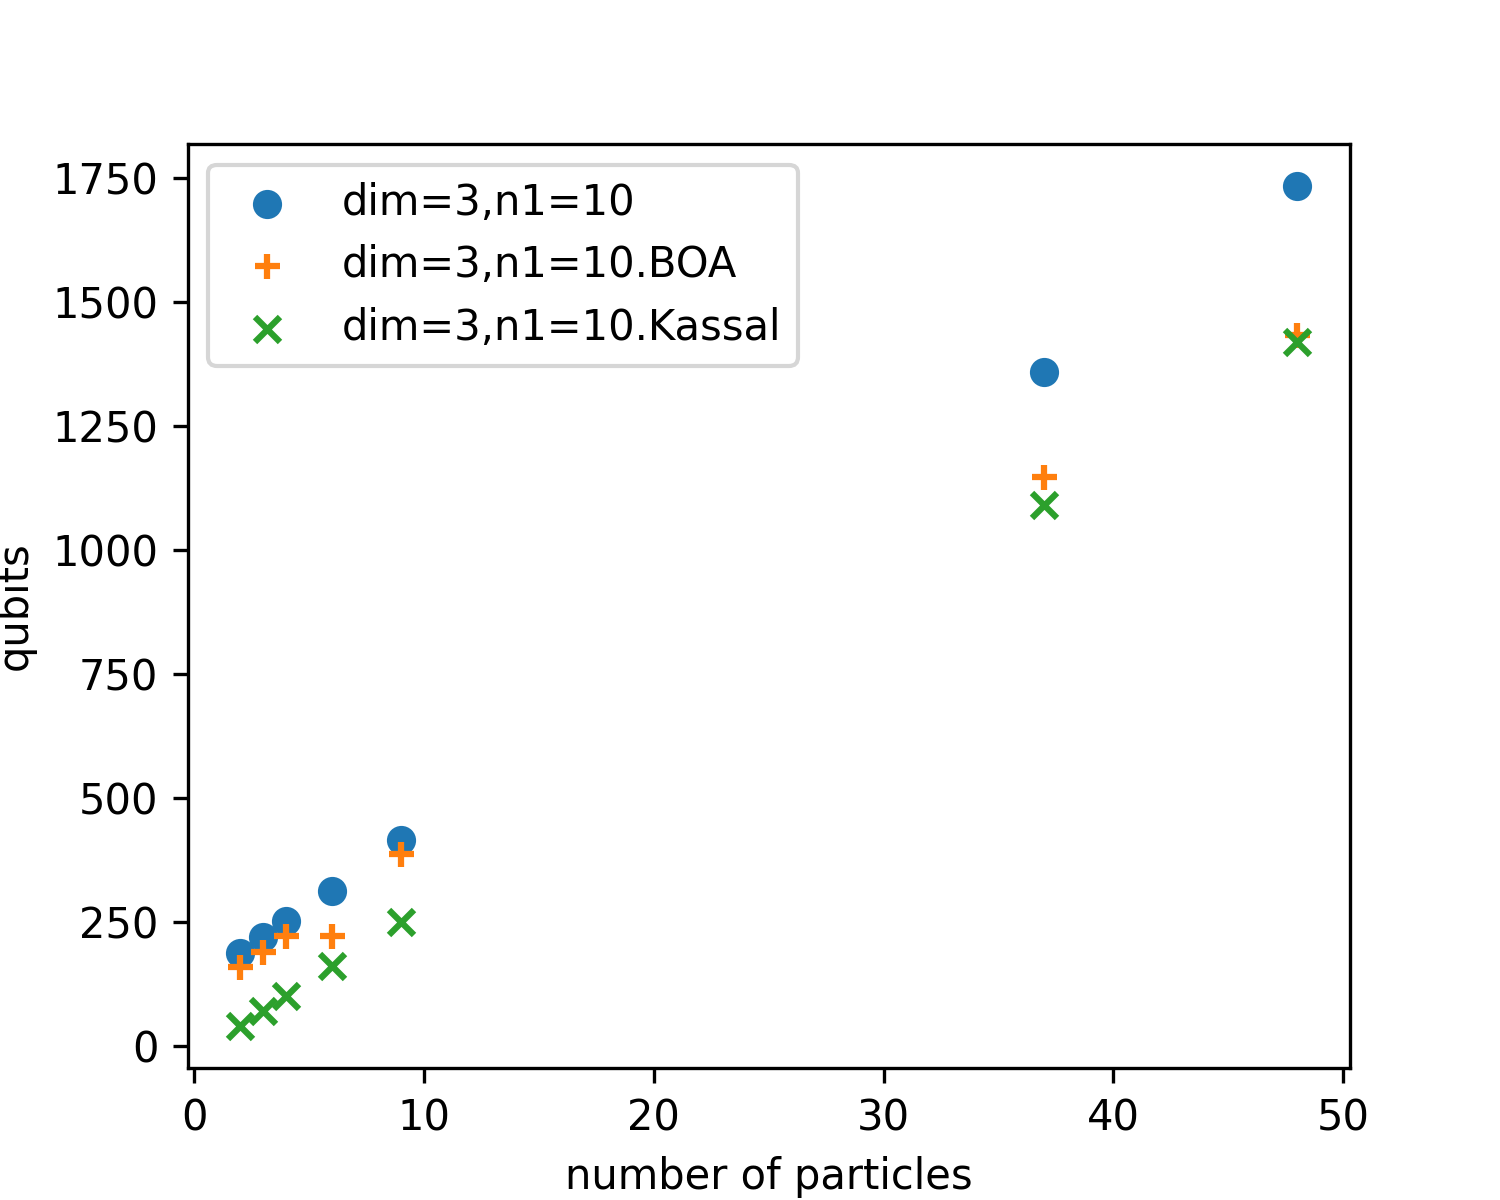
\includegraphics[width=0.6\textwidth]{paper2025_figs/circuit-size-qubits.png}
    \caption{Relationship between particle number and qubit count}
    \label{fig:qubit-for-some-molecules}
    \begin{flushleft}\small

        The relationship between particle count and qubit count is shown for
        several molecules with different particle numbers. Particle number is
        the sum of electron number and atom number. The points correspond, in
        ascending particle number, to \ce{H}, \ce{He}, \ce{Li}, \ce{H + H2},
        \ce{O}, glycine (\ce{C2H5NO2}), and alanine (\ce{C3H7NO2}). Points
        marked with \verb|+| are values under fixed nuclear positions
        (Born-Oppenheimer approximation: BOA). Points marked with \verb|x| are
        values from the formula reported by
        Kassal \cite{kassal2008.pnas.0808245105}.
    \end{flushleft}
\end{figure}

Figure \ref{fig:qubit-for-some-molecules} shows the relationship between
particle number and qubit count when simulator circuits are generated by our
circuit generator for several atoms or molecules. This figure ignores emulator
executability and assumes unconstrained qubit usage. Coordinate qubit count is
set to 10 bits and calculations are for three-dimensional models using
arithmetic gates. The required qubit count scales linearly with particle number.
\clearpage


\section{Treatment of the Coulomb-Potential Pole}
\label{sec:coulomb-potential-handling}
In this study, we compute the Coulomb potential with quantum circuits because we
target atomic models. In Hamiltonian simulation for atomic models, one must
define how to treat the pole of the Coulomb potential. In time-evolution
calculation, the product of potential $-1/r$ and wavefunction $\psi$ is computed
at each grid coordinate. If this product is evaluated at the potential pole, it
diverges. Countermeasures can be broadly classified into two categories:
(a) introducing an approximate potential expression that does not diverge even
when interparticle distance is zero, and
(b) redefining coordinate discretization of nucleus and electron so that their
distance does not become zero in computation. For (a), we examine two example
approximations. The first approximation (a1) uses the average potential energy
within the grid cell containing the pole as the representative value for that
cell. The second approximation (a2) is a potential function that adds an offset
term to the norm used in interparticle-distance calculation, known as a soft-
core potential. This function has also been studied as a way to prevent
divergence of Coulomb-term calculation in Hamiltonian simulation
\cite{Childs2022quantumsimulationof,Kivlichan_2017},
and has also been analyzed as a model for physical systems with constrained
electron motion \cite{Hall2009.PhysRevA.80.032507,
Fernandez_1991, LiChen2021.doi:10.1021/acs.jpca.1c00698}.

As an example of method (b), it has been proposed to define electron positions
at grid centers while defining nuclear coordinates shifted by half a grid step
along one axis from those centers \cite{Chan2023.sciadv.abo7484}. In that
approach, Trotter error becomes large near the potential pole, so Chan et al.
apply post-processing correction to computed results. In this study, we do not
adopt method (b).

In the potential-energy-term circuit $\Thetaep$ of the time-evolution operator,
the product of Coulomb potential and wavefunction value is computed. This is
problematic when the wavefunction value is nonzero at the potential pole.
Among the wavefunctions considered in this report, the affected cases are the
two-dimensional solutions with azimuthal quantum number $m=0$:
$\Psi_{0,0}^{\mathrm{2D}}$ and $\Psi_{1,0}^{\mathrm{2D}}$.

\subsection{Approximation Using a Representative Value for the Pole-Containing Cell}
Approximation (a1) uses the original expression away from the pole coordinate,
and returns a finite value at the pole:
it is defined as follows with value $-1/\Delta_1$ at the pole.
\begin{equation}
\HaOne(r) = \begin{cases}
-\frac{1}{r} & (r>0) \\
-\frac{1}{\Delta_1} & (r=0)
\end{cases}\label{eq:Ha1r}
\end{equation}
$\HaOne$ has low circuit-implementation cost. In the fixed-point division
circuit implemented in this study, division by zero yields the maximum
representable value, i.e., all bits equal to 1. If this value can be directly
used as $1/\Delta_1$, no additional circuit component is needed. For potential
calculation, division uses fixed-point format with one integer bit and $\nb$
fractional bits. The all-ones value is
$(2^{\nb+1}-1)\times2^{-\nb}=1.11\ldots1_2\simeq2_{10}$. This means that at
$r=0$, the computed value of $1/r$ is approximately 2. Considering that the
unit of $r$ is $\deltar$, this corresponds to the value at $r=\deltar/2$, i.e.,
choosing $\Delta_1=\deltar/2$.

First, we describe how to choose $\Delta_1$ in $\HaOne$. Here we show a
derivation for the case where the wavefunction is known.

In the one-dimensional model $\PsiOneD_1$, the wavefunction value at the
potential pole is zero, so it is sufficient that the potential value be finite;
therefore we use $\Delta_1=\deltar/2$, which requires no additional circuit for
the approximation.

In the two-dimensional model, depending on azimuthal quantum number $m$, the
wavefunction value at the pole may be zero or nonzero. Solutions with $m\ne0$
are zero at the pole, while those with $m=0$ are nonzero. We consider
$\PsiTwoD_{0,0}$ and $\PsiTwoD_{1,0}$ as nonzero examples and examine an
appropriate potential value at $r=0$. Since the representative value may be
chosen arbitrarily when $m=0$, the $\Delta_1$ value derived for one case can
also be applied to the other.

The parameter $\Delta_1$ in approximation $\HaOne$ can be determined as follows.
In Coulomb-term calculation, the potential value at each grid-cell center is
used as a representative value, and multiplied by grid-cell area to approximate
the integral. At a grid point coinciding with the pole, this representative
value diverges; however, the integral of the average over the cell region does
not diverge in two-dimensional or higher-dimensional models. Therefore, we
define the potential approximation at the pole by choosing a representative
value that reproduces the integral value.

Consider the inscribed circle of the grid cell centered at the pole. Let the
representative Coulomb-potential value within that circle be $-1/\Delta_1$, and
compute the corresponding energy value $W_{n,m}^\prime$. Next, compute the
energy value $W_{n,m}$ over the same region using the true Coulomb potential.
Then determine $\Delta_1$ such that the two values match. We perform this for
$(n,m)=(0,0)$ and $(1,0)$. The expressions for $W_{n,m}$ and
$W_{n,m}^\prime$ are:
\begin{align}
    W_{n,m}&=\int_{\theta=0}^{2\pi}d\theta\int_{r=0}^{\deltar/2}
    \Hep(r)\abs{\PsiTwoD_{n,m}(r)}^2r dr\\
    W_{n,m}^\prime&=\pi\left(\frac{\deltar}{2}\right)^2
    \HaOne(0)\PsiTwoD_{n,m}(0) \notag \\
    &=-\frac{\pi\deltar^2}{4\Delta_{1,n,m}}
    \sqrt{\frac{q_0^3(n-\abs{m})!}{\pi(n+\abs{m})!}}
    L_{n-\abs{m}}^{2\abs{m}}(0)
\end{align}
For $(n,m)=(0,0)$ and $(1,0)$, solving $W_{n,m}=W_{n,m}^\prime$ gives
\begin{align}
    \Delta_{1,0,0} &=\frac{q_0\deltar^2}{4(-e^{-q_0\deltar}+1)}
    \simeq \frac{q_0\deltar^2}{4(-1+q_0\deltar+1)}=\frac{\deltar}{4}
    \label{eq:delta-1-0-0}\\
    \Delta_{1,1,0} &=\frac{q_0\deltar^2}{4((-1+q_0^2\deltar^2)e^{-q_0\deltar}+1)}
    \simeq \frac{q_0\deltar^2}{4((-1+q_0^2\deltar^2)(1-q_0\deltar)+1)}
    \simeq\frac{\deltar}{4}
    \label{eq:delta-1-1-0}
\end{align}
These approximations are valid when $\deltar\ll1$. Derivations are shown in
Appendix \ref{chap:appendix_derivation_derivation}.

Figure \ref{fig:Ha1-vs-delta1} shows energy values computed for several values
of $\nb$ while varying $\Delta_1$ in $\HaOne(r)$ using
$1/a=\deltar/\Delta_1$ over $1\le a\le8$. Because these plots include
conditions beyond simulator-circuit executable ranges, values were computed
with an equivalent classical program rather than quantum circuits. As seen in
Figure \ref{subfig:Ha1-energy-0-0} and \ref{subfig:Ha1-energy-1-0}, for both
$\PsiTwoD_{0,0}$ and $\PsiTwoD_{1,0}$, results are nearly identical to
analytical energy eigenvalues at $a=4$, i.e., $\Delta_1=\deltar/4$. In all
plots, error sign flips around $a=4$. In Eq. (15), the approximation for
$\deltar\ll1$ gives $\deltar/4$; the graphs show increasing error away from
$\deltar/4$, indicating a common optimal condition across bit counts.

\begin{figure}[ht]
    \centering
    \begin{subfigure}{0.45\columnwidth}
        \centering
        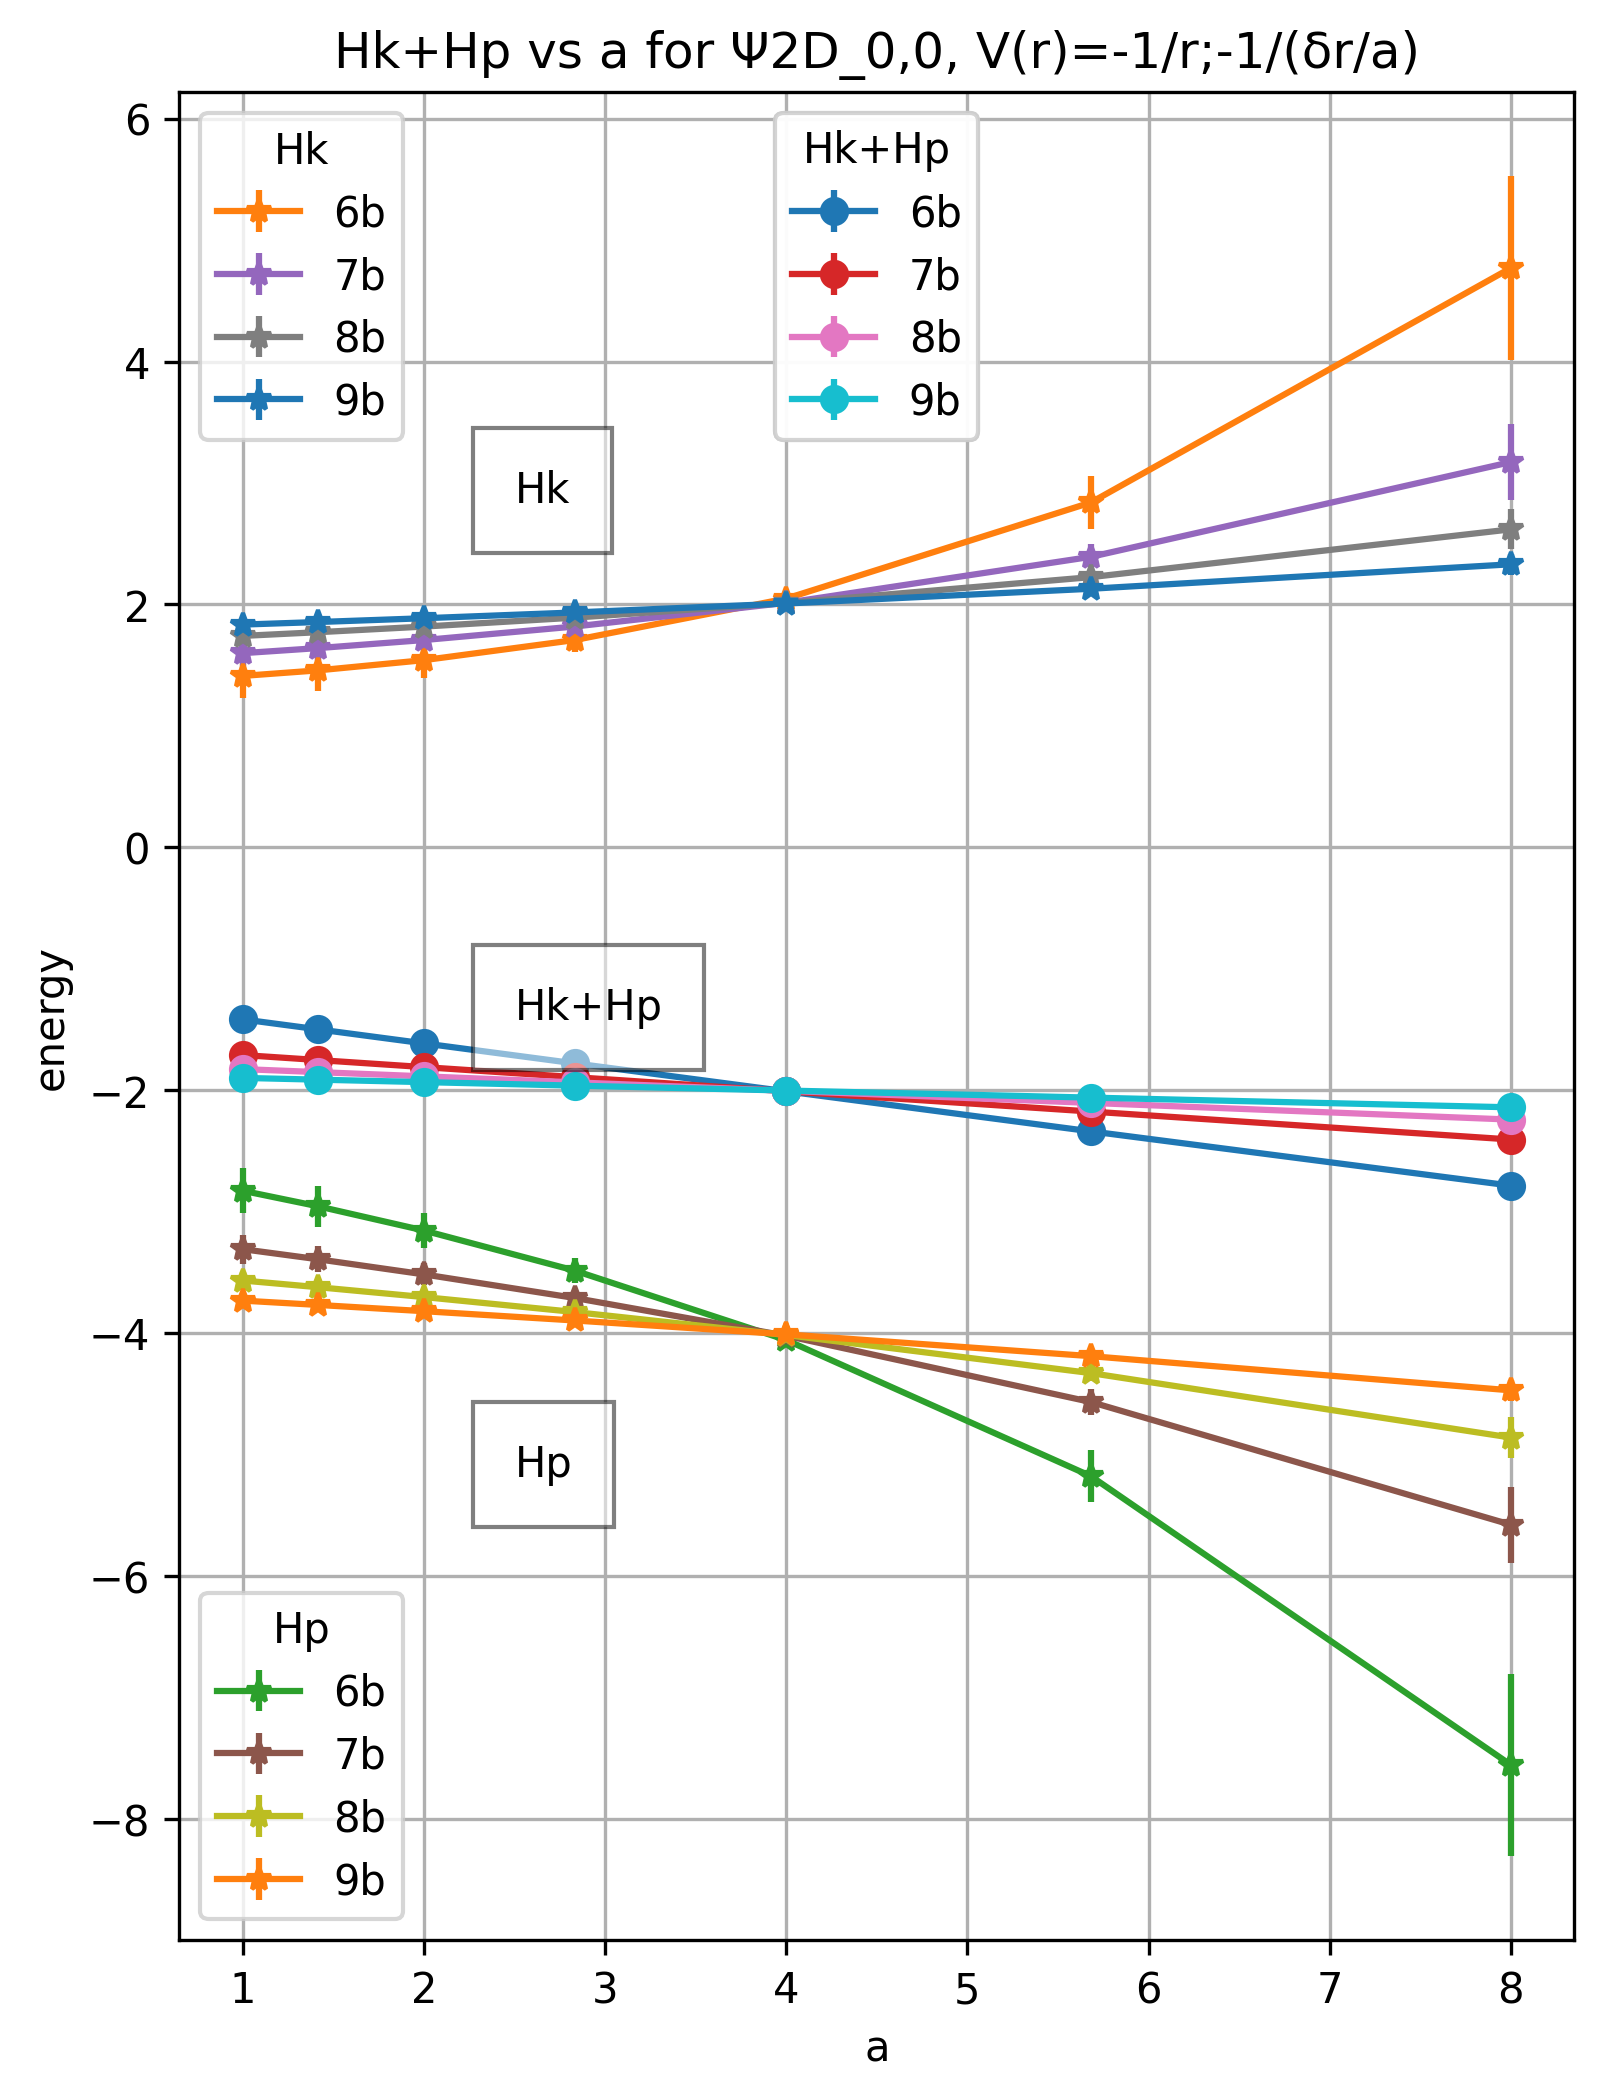
\includegraphics[width=1\columnwidth]{paper2025_figs/compare_energy/compare_energy_h2D_TO2_r0lim_0_0.png}
        \caption{$\PsiTwoD_{0,0}$}
        \label{subfig:Ha1-energy-0-0}
    \end{subfigure}
    \begin{subfigure}{0.47\columnwidth}
        \centering
        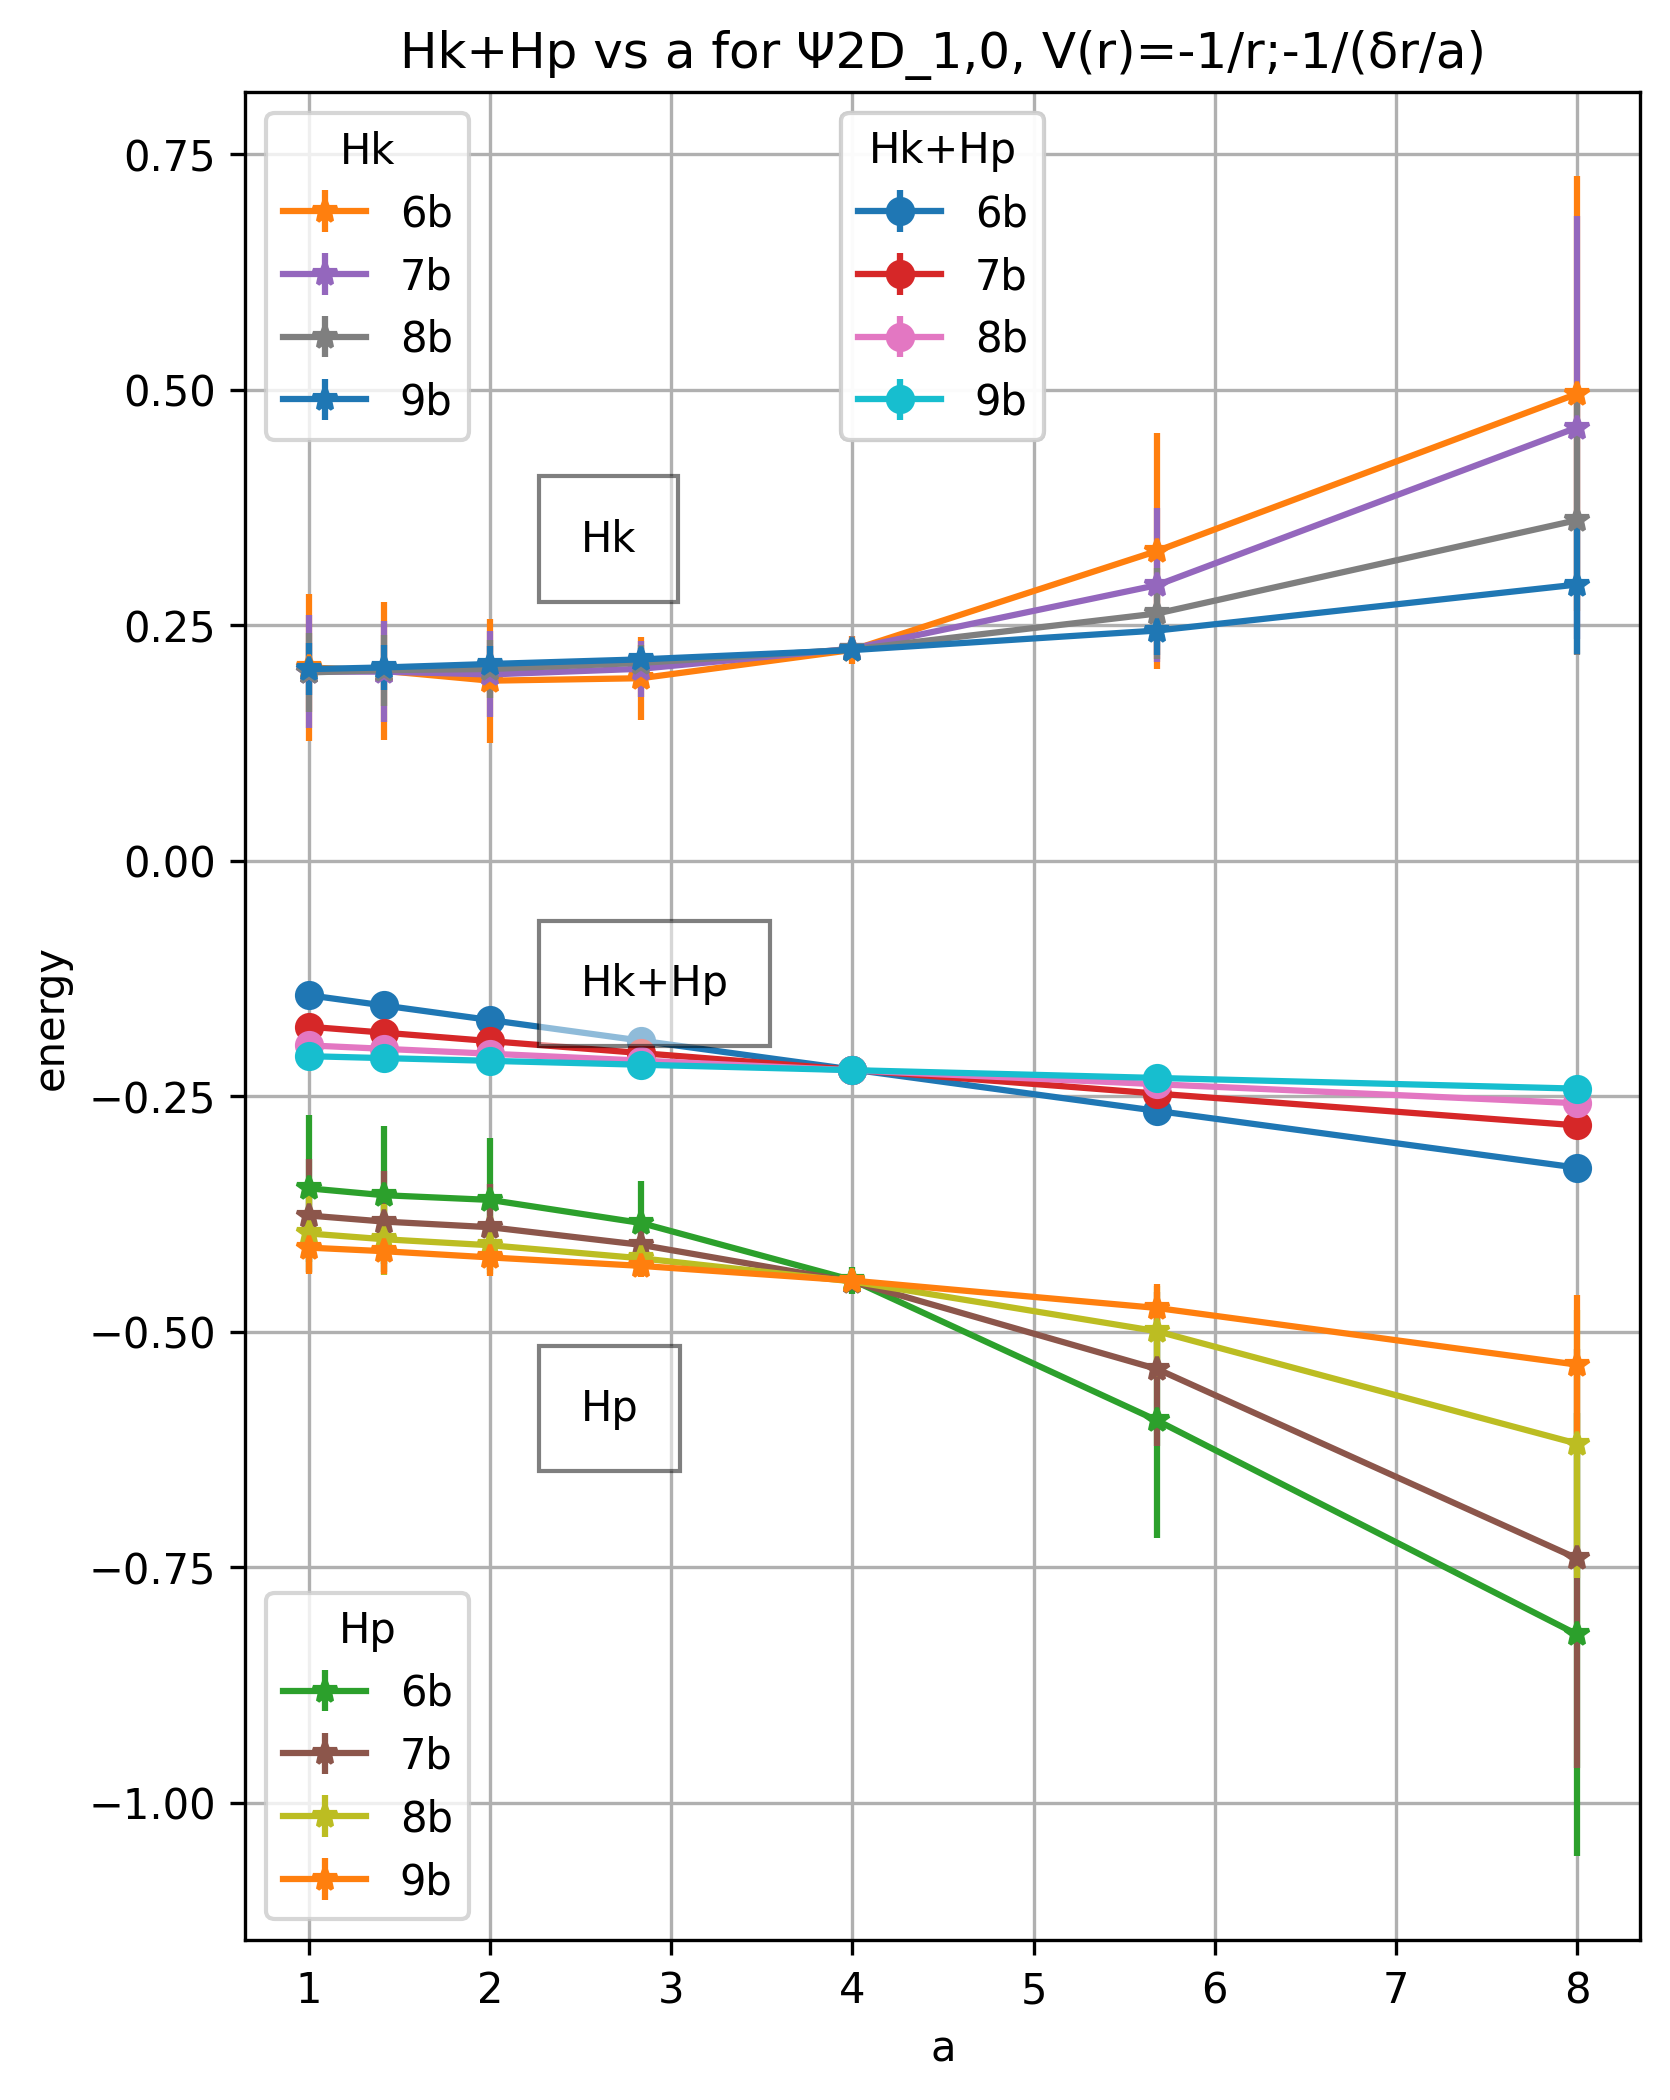
\includegraphics[width=1\columnwidth]{paper2025_figs/compare_energy/compare_energy_h2D_TO2_r0lim_1_0.png}
        \caption{$\PsiTwoD_{1,0}$}
        \label{subfig:Ha1-energy-1-0}
    \end{subfigure}
    \caption{Energy-value variation versus $\Delta_1$ in approximation $\HaOne(r)$}
    \label{fig:Ha1-vs-delta1}
    \begin{flushleft}\small
        (a) Plot for $\PsiTwoD_{0,0}$ with $\Delta_1=\deltar/a$ while varying
        $a$. Values of $a$ follow a geometric series with ratio $\sqrt{2}$. For
        all bit counts, at $a=4$ (i.e., $\Delta_1=\deltar/4$), $\Hk+\Hp$ is
        close to the analytical energy eigenvalue $-2.0$. (b) Plot for
        $\PsiTwoD_{1,0}$, where at $a=4$ the value is also close to the
        analytical energy eigenvalue $-0.2222$.
    \end{flushleft}
\end{figure}

\clearpage
\subsection{Approximation Using a Soft-Core Potential}
Approximation (a2) is a soft-core potential expression that adds an offset term
to the norm used in distance calculation, defined as follows
\cite{Kivlichan_2017}.
\begin{equation}
\HaTwo(r) = -\frac{1}{\sqrt{r^2+\Delta_2^2}}\label{eq:Ha2r}
\end{equation}

Figure \ref{fig:Ha2-vs-delta2} shows energy values for $\HaTwo(r)$ while
varying constant $\Delta_2$ in the expression. These values were computed by a
classical program rather than simulator circuits.

At $r=0$, $\HaTwo(0)=-1/\Delta_2$, which is the same form as $\HaOne(r)$.
Accordingly, as with $\HaOne(r)$, values close to analytical energy eigenvalues
are obtained when $\Delta_2=\deltar/4$. For $r\ne0$, the two expressions differ,
but the computed energy values show no large difference. As seen in the plots
of Figure 8, for $\HaTwo(r)$ as well, values close to analytical energy
eigenvalues are obtained at $\Delta_2=\deltar/4$.

\begin{figure}[ht]
    \centering
    \begin{subfigure}{0.45\columnwidth}
        \centering
        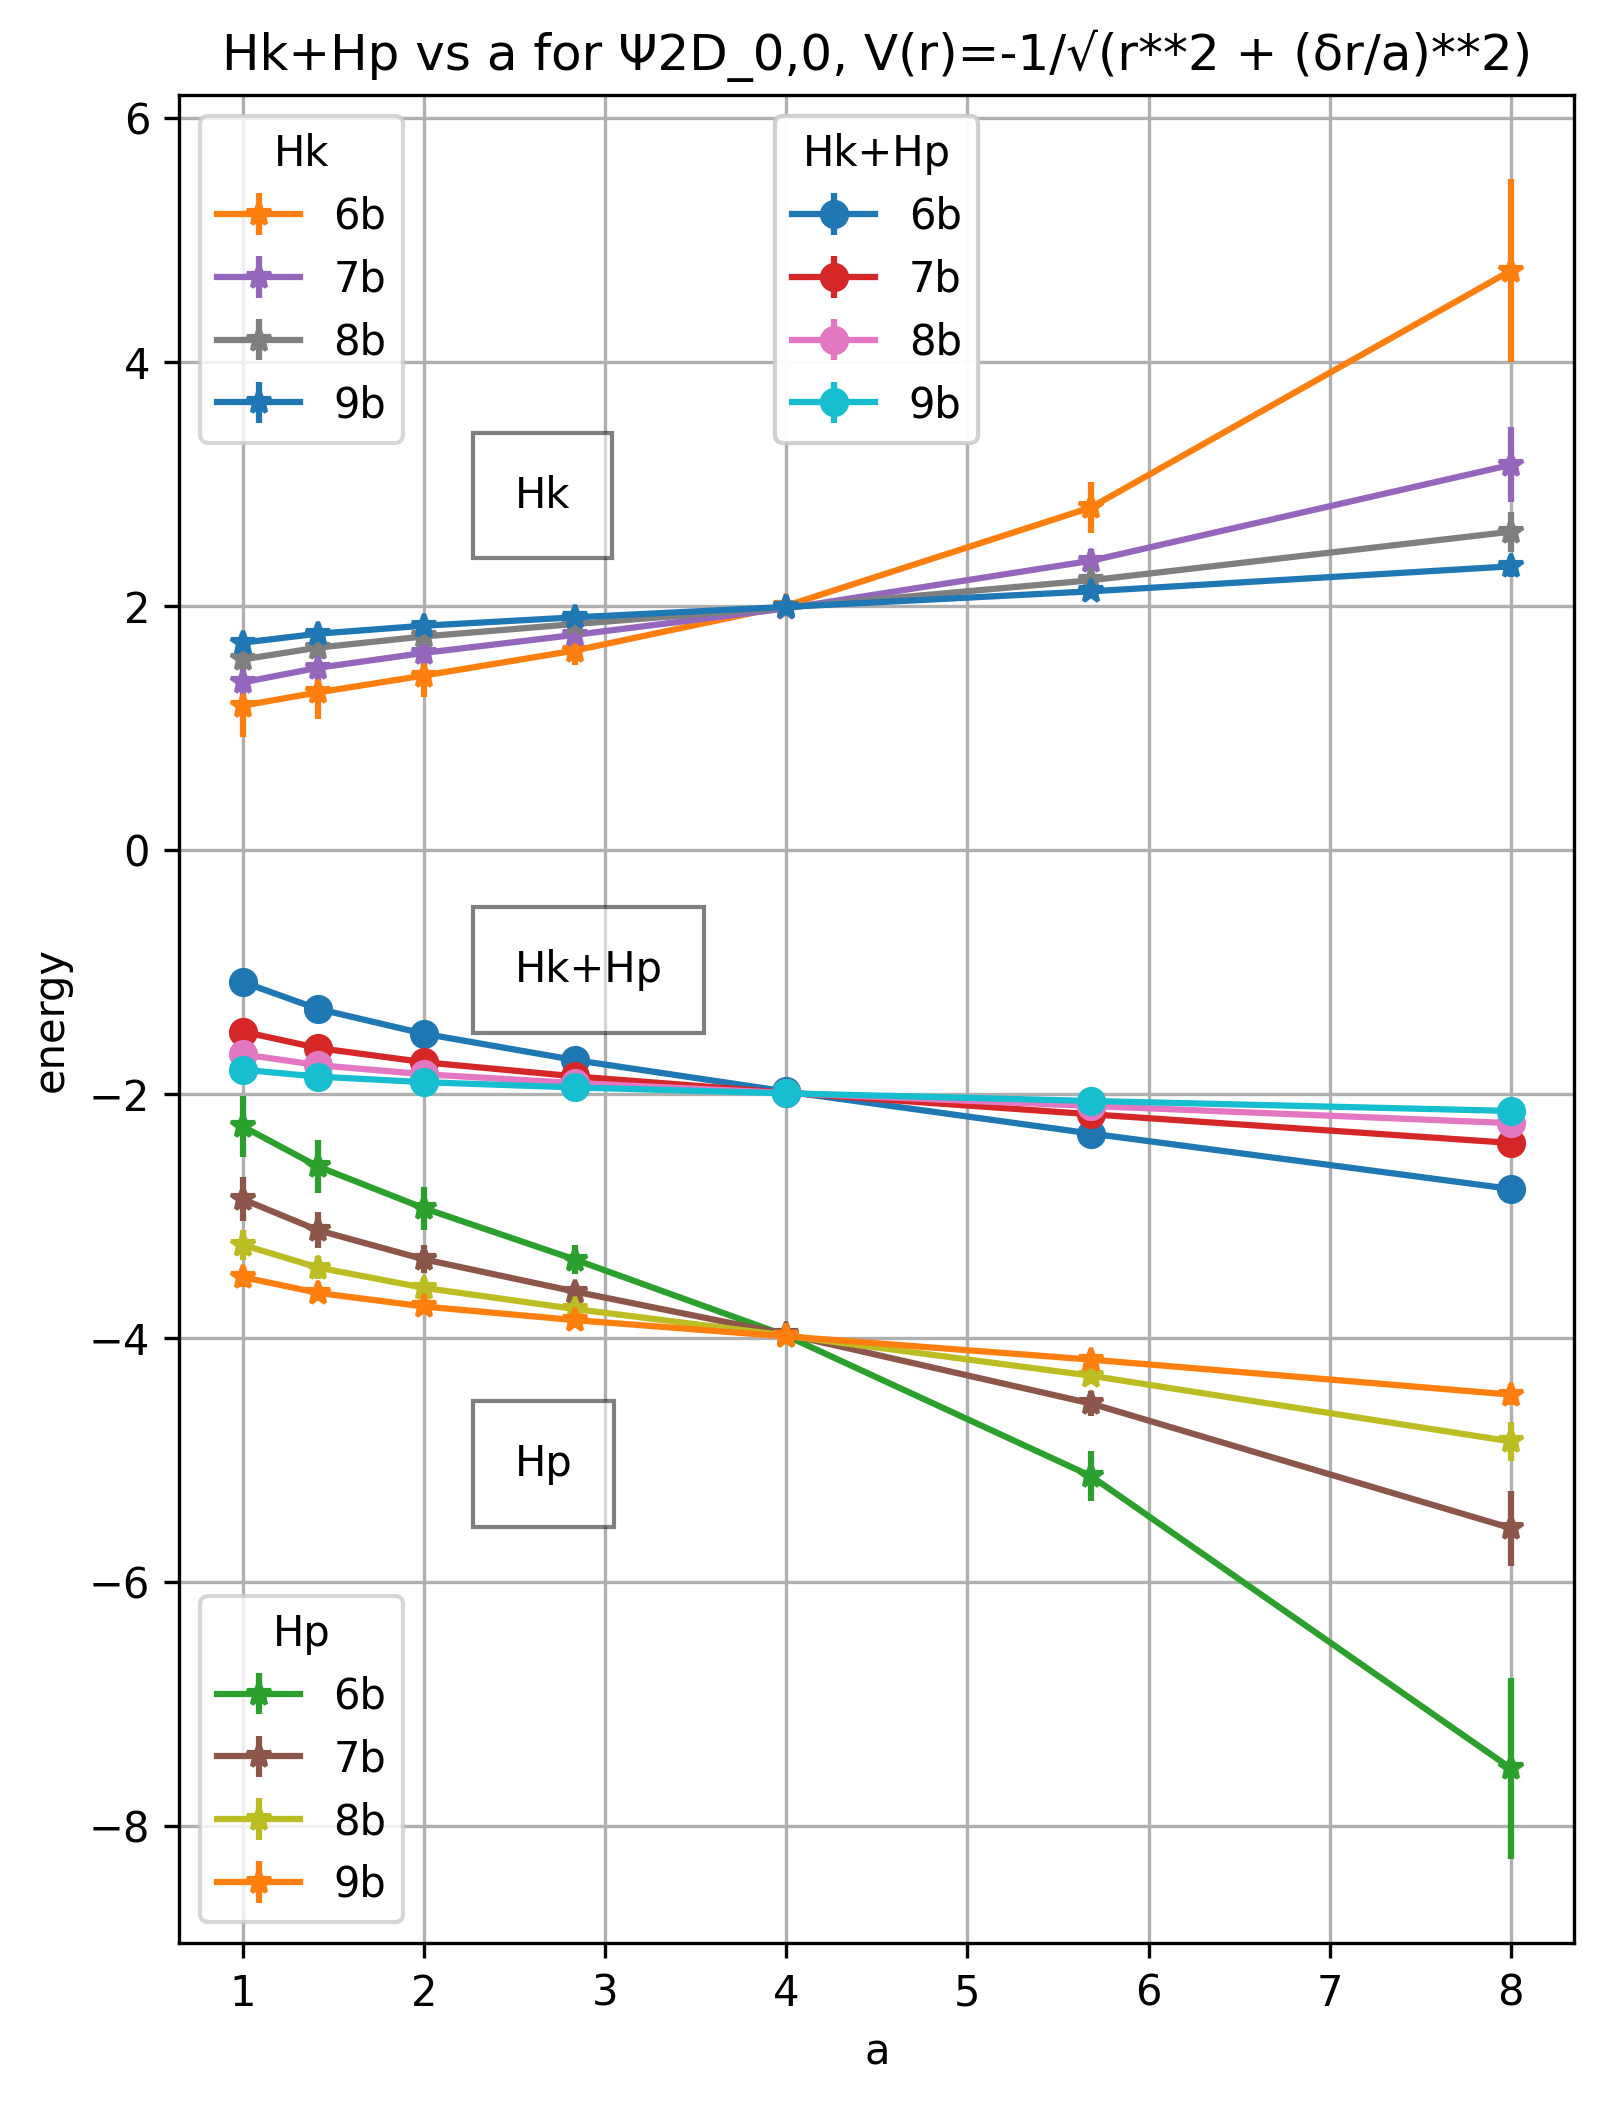
\includegraphics[width=1\columnwidth]{paper2025_figs/compare_energy/compare_energy_h2D_TO2_rofs_0_0.png}
        \caption{$\PsiTwoD_{0,0}$}
        \label{subfig:Ha2-energy-0-0}
    \end{subfigure}
    \begin{subfigure}{0.47\columnwidth}
        \centering
        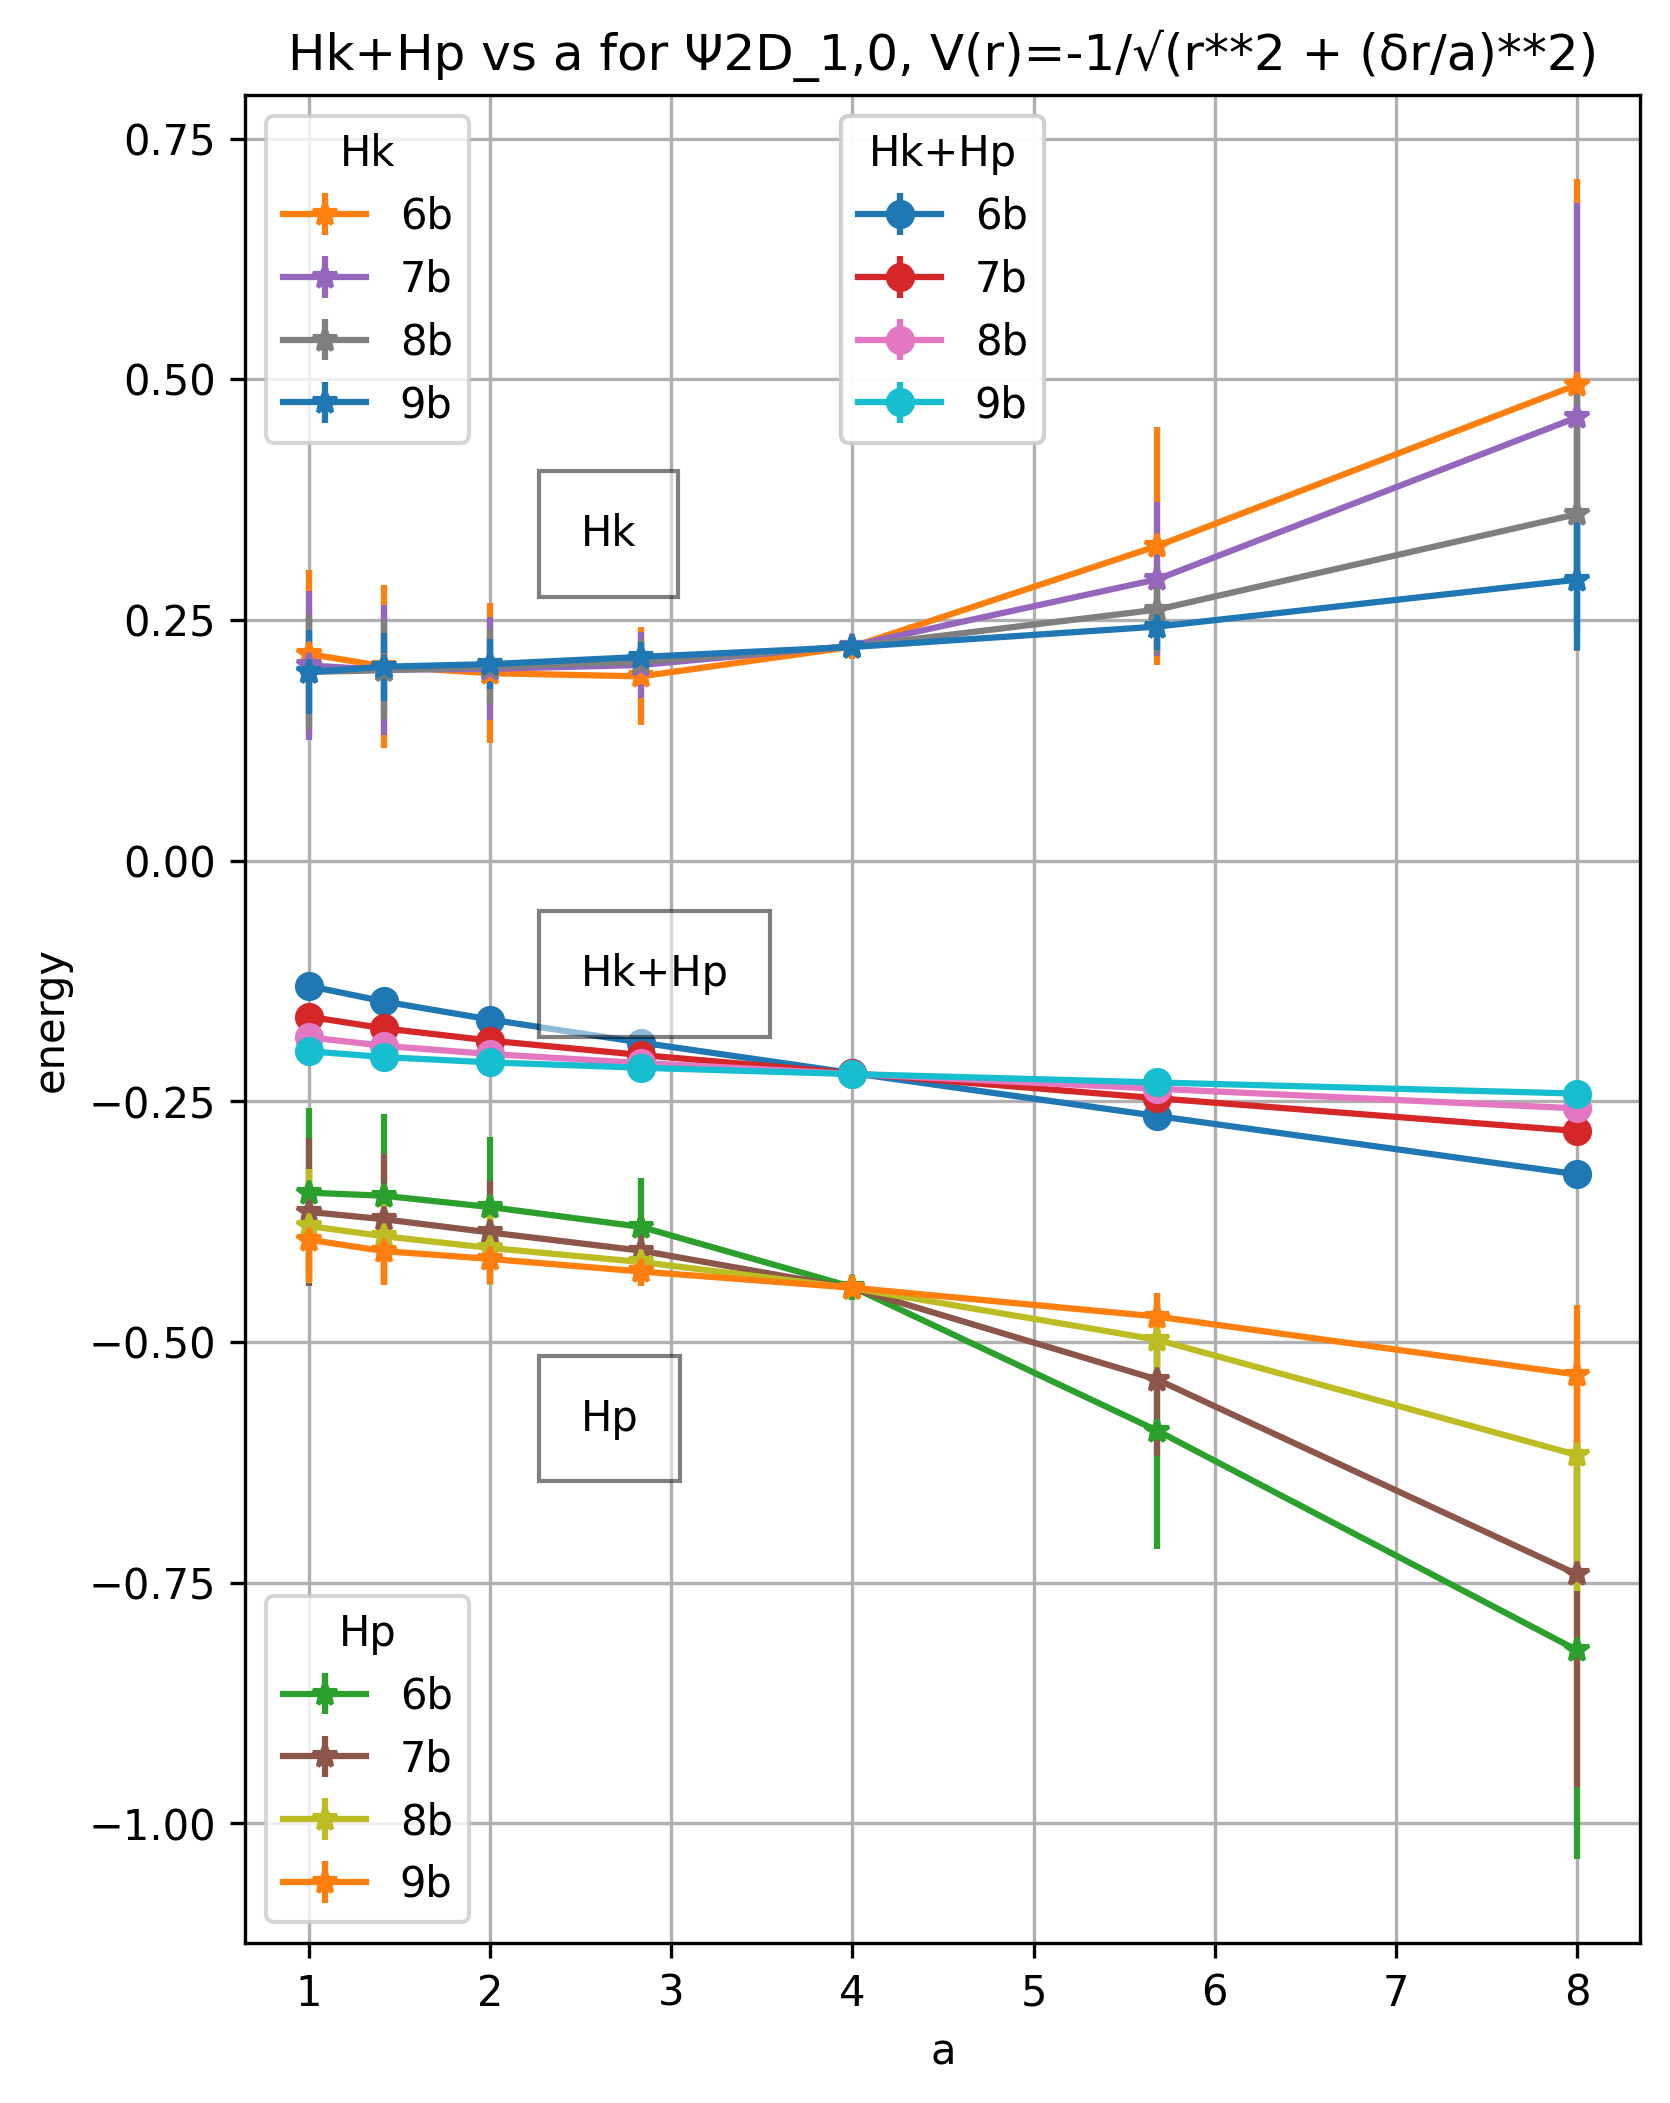
\includegraphics[width=1\columnwidth]{paper2025_figs/compare_energy/compare_energy_h2D_TO2_rofs_1_0.png}
        \caption{$\PsiTwoD_{1,0}$}
        \label{subfig:Ha2-energy-1-0}
    \end{subfigure}
    \caption{Energy-value variation versus $\Delta_2$ in approximation $\HaTwo(r)$}
    \label{fig:Ha2-vs-delta2}
    \begin{flushleft}\small

        (a) Plot for $\PsiTwoD_{0,0}$ with $\Delta_2=\deltar/a$ while varying
        $a$. Values of $a$ follow a geometric series with ratio $\sqrt{2}$. For
        all bit counts, at $a=4$ (i.e., $\Delta_2=\deltar/4$), $\Hk+\Hp$ is
        close to the analytical energy eigenvalue $-2.0$. (b) Plot for
        $\PsiTwoD_{1,0}$, where at $a=4$ the value is also close to the
        analytical energy eigenvalue $-0.2222$.

    \end{flushleft}
\end{figure}

\clearpage

\section{Determination of Simulation Parameters for Minimum Error}
\label{sec:parameter-selection-for-minimum-error}
Hamiltonian simulation requires setting several simulation parameters. Spatial
resolution and time-step selection for controlling computational error have been
extensively studied, including estimation of the qubit count required for a
target precision \cite{FEIT1982412, Kivlichan_2017,
Chan2023.sciadv.abo7484}. In contrast to these existing studies, this report
focuses on constraints and trade-offs imposed on simulation parameters when the
qubit count is fixed, and investigates how to determine parameter values that
yield the best accuracy. In this report, time evolution uses Trotter
decomposition. For models defined on grids and evolved with Trotter
decomposition, the resulting wavefunction includes the following errors.

\begin{equation}
\errtotal \leq \errspatial + \errtemporal
\label{eq:error-total-decomposition}
\end{equation}

Here, $\errtotal$ is total error, $\errspatial$ is error due to spatial
discretization parameters, and $\errtemporal$ is error due to temporal
discretization parameters. Both can be further decomposed. Although
characteristics of each component are known, improving only one component may
not improve total error when other components dominate. Therefore, dominant
error terms must be reduced while considering trade-offs.

The trade-off examined here is the relationship between spatial grid spacing
$\deltar$ and side length $L$ of the simulation-domain box. In the grid method,
one defines a box-shaped computational domain and computes the wavefunction only
within that domain. Amplitudes outside the domain are ignored, so to achieve
desired accuracy, the domain must be large enough that boundary amplitudes are
negligible. As one criterion for whether side length $L$ is sufficient for a
target precision, it has been proposed to numerically compute the maximum
electron density on domain boundaries and choose $L$ so that it is below a
target value $\rho_0$ \cite[Supplementary material, S8, A. Space
Cost]{Chan2023.sciadv.abo7484}. To increase $L$, one must either increase qubit
count or coarsen resolution. In high-qubit environments, qubit count can be
increased as needed; under constrained qubit counts, one must instead increase
$\deltar$. In that case, spatial size and resolution are in trade-off.
Concrete methods for dimension selection under this trade-off have not been
fully discussed. Here, assuming a wavefunction, we numerically evaluate this
trade-off and present a method for selecting suitable parameter values.

The time step $\deltat$ must satisfy two conditions: one based on the sampling
theorem via discrete Fourier transform \cite{FEIT1982412}, and one derived from
Trotter-decomposition error
\cite{Childs2021.PhysRevX.11.011020,Burgarth2024.PhysRevResearch.6.043155}.
Both must be considered.

Equation \ref{eq:error-total-decomposition}, which separates errors into spatial-
parameter and temporal-parameter contributions, can be further decomposed as
follows.
\begin{align}
    \errspatial &\equiv \errdisc + \errcutoff \\
    \errtemporal &\equiv \erralias + \errtrotter
\end{align}
Here, $\errdisc$ is wavefunction approximation error due to spatial
discretization, and $\errcutoff$ is error due to wavefunction components outside
the computational box. $\erralias$ is aliasing error caused by finite-term
wave-number representation, and $\errtrotter$ is error due to Trotter
approximation.

In this section, we present how to choose parameters to reduce these errors when
the total qubit count is fixed. The two spatial-parameter errors,
$\errdisc$ and $\errcutoff$, are in trade-off, so we discuss how to determine
$\deltar$ under that trade-off. For temporal parameter $\deltat$, no trade-off
exists; the sampling theorem provides an upper bound on $\deltat$, and
analytical Trotter-error evaluation provides an upper bound on expected error.
We determine parameters by considering both.

\subsection{Method for determining the grid size}
\label{subsec:delta-r-selection-method}
In this report, periodic boundary conditions are applied to the simulation
domain, and side length is common across dimensions: $L=2^{\nb}\deltar$. The
space center is set as the coordinate origin, with the nucleus placed at the
origin. Wavefunction components outside $[-L/2,L/2]$ are cutoff. Choosing a
smaller $\deltar$ is favorable for reducing $\errdisc$, but because $L$ also
shrinks proportionally with $\deltar$, $\errcutoff$ increases. By finding
$\deltar$ where $\errdisc$ and $\errcutoff$ within the computational domain
balance each other, one can obtain the $\deltar$ that minimizes their total.

Let $S_1$ be the integral of squared wavefunction over the simulation domain and
$S_2$ the integral outside the domain:
\begin{align}
S_1 &= \int_{x,y,z=-L/2}^{L/2}\Psi(\bm{r})^{\ast}\Psi(\bm{r}) d\bm{r} \\
S_2 &= 1 - S_1
\end{align}


Let $S_d$ be the corresponding approximation on discretized coordinates:
\begin{equation}
S_d = \sum_{j}\abs{\Psi(\chij)}^2 \deltar^3
\end{equation}
Then,
\begin{align}
\errdisc &\simeq \abs{S_1 - S_d} \label{eq:err-disc-definition}\\
\errcutoff &\simeq S_2 \label{eq:err-cutoff-definition}
\end{align}
The $\deltar$ that minimizes $\abs{S_d-S_1}+S_2$ is the optimal value.

With coordinate qubit count $\nb$ fixed, varying spatial-discretization
parameter $\deltar$ keeps grid count $2^{(\nb)}$ constant, so
$L=2^{(\nb)}\deltar$ changes simultaneously. Larger $\deltar$ increases
discretization error $\errdisc$, while smaller $L$ increases cutoff error
$\errcutoff$. Therefore, $\deltar$ must be chosen by considering the trade-off
between these two errors.

Figure \ref{subfig:dq-tradeoff-1d} compares discretization error
$\errdisc=|S_d-S_1|$ and cutoff error $\errcutoff=S_2$ for several values of
$\nb$ in the one-dimensional model $\psi_1^{1D}$.

Focusing on $\nb=6$, which has the fewest grid points, panel (A1) shows that the
$S_2$ line and $|S_d-S_1|$ line intersect around $\deltar=0.22$. In panel (A2),
this corresponds to the minimum point of the $\nb=6$ curve. This value is where
the trade-off between the two error types is balanced. Since $\deltar$ and $L$
are proportional, panel (A3) indicates $L=14$ at that point.

For the $\nb=8$ case (two more qubits), panel (A2) shows that values are nearly
zero over $\deltar=0.07\sim0.14$. This means that varying $\deltar$ in this
range does not noticeably change error. The sharp decrease for $\deltar<0.07$
occurs because smaller $L$ makes cutoff error significant. The increase for
$\deltar>0.14$ occurs because discretization error becomes significant. As qubit
count increases, the range of $\deltar$ giving near-minimum values in (A2)
widens, allowing more flexible choice of $\deltar$.

Figures \ref{subfig:dq-tradeoff-2d-0-0} and
\ref{subfig:dq-tradeoff-2d-1-0} show corresponding plots for the two-
dimensional wavefunctions $\Psi_{0,0}^{2D}$ and $\Psi_{1,0}^{2D}$. They show
that the suitable range of $\deltar$ changes substantially depending on spatial
spread of the wavefunction.

\begin{figure}[ht]
    \centering
    \begin{subfigure}{1.0\columnwidth}
        \centering
        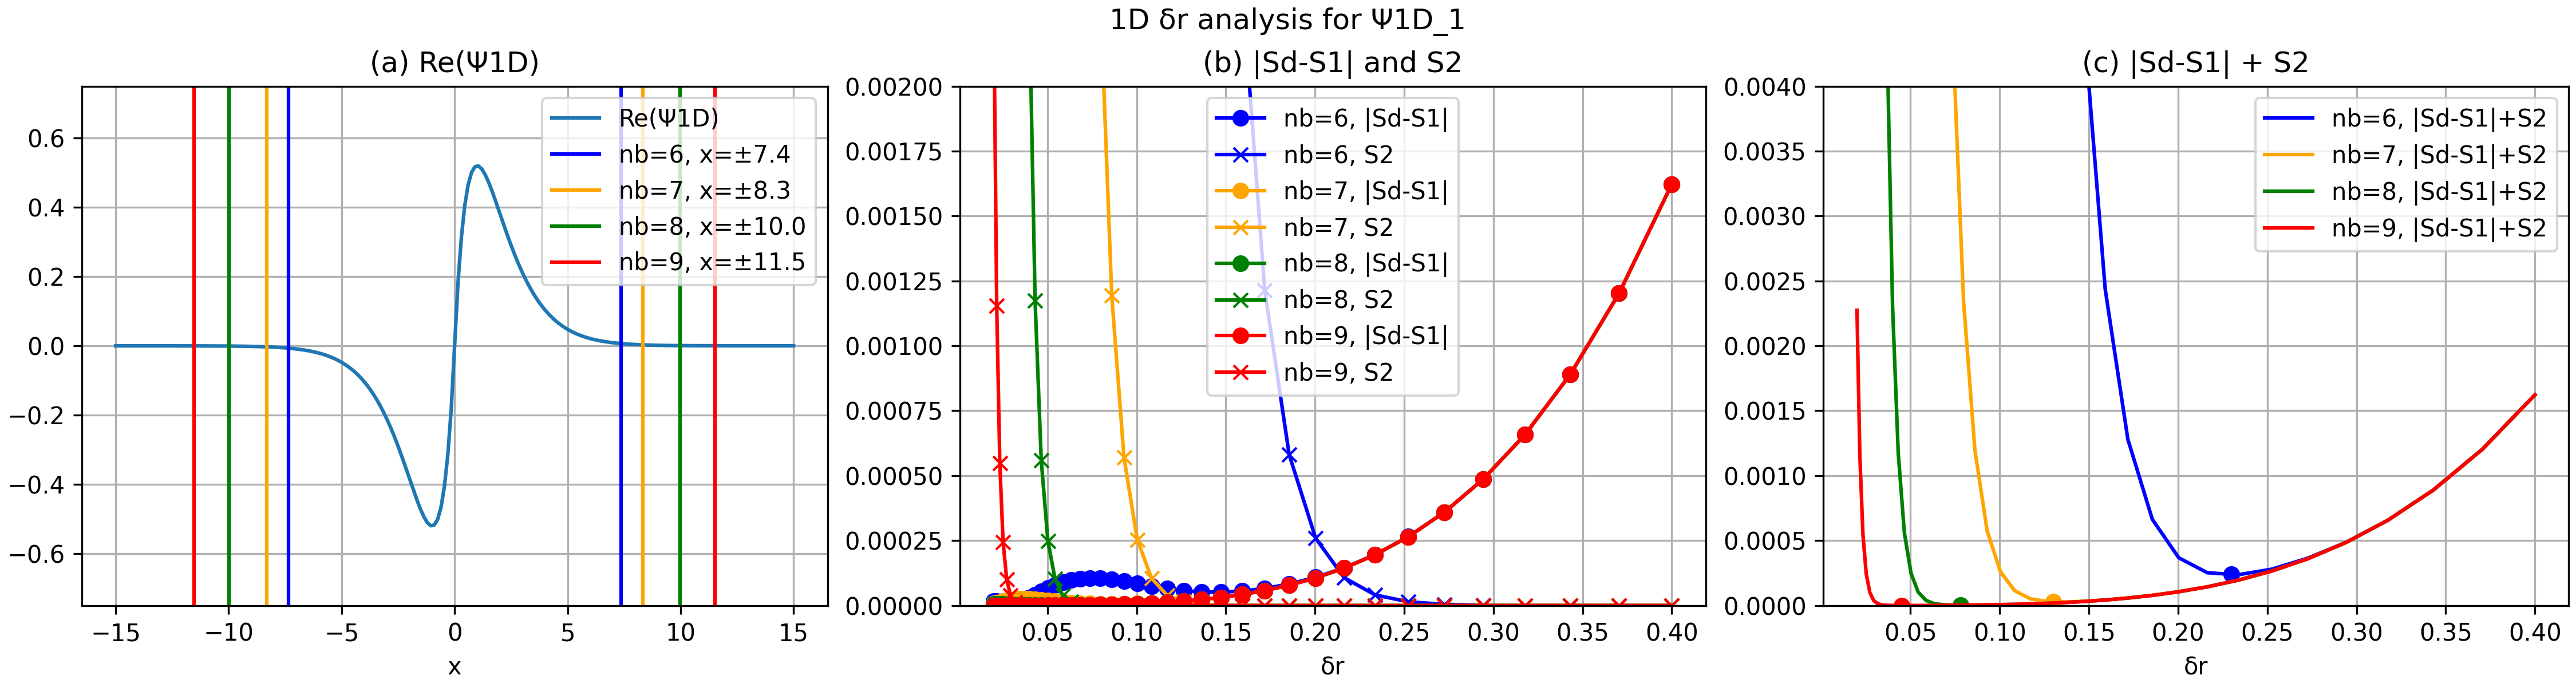
\includegraphics[width=\columnwidth]{paper2025_figs/dq_tradeoff/eval1d_dq.png}
        \caption{One-dimensional model $\PsiOneD_1$}
        \label{subfig:dq-tradeoff-1d}
    \end{subfigure}
    \begin{subfigure}{1.0\columnwidth}
        \centering
        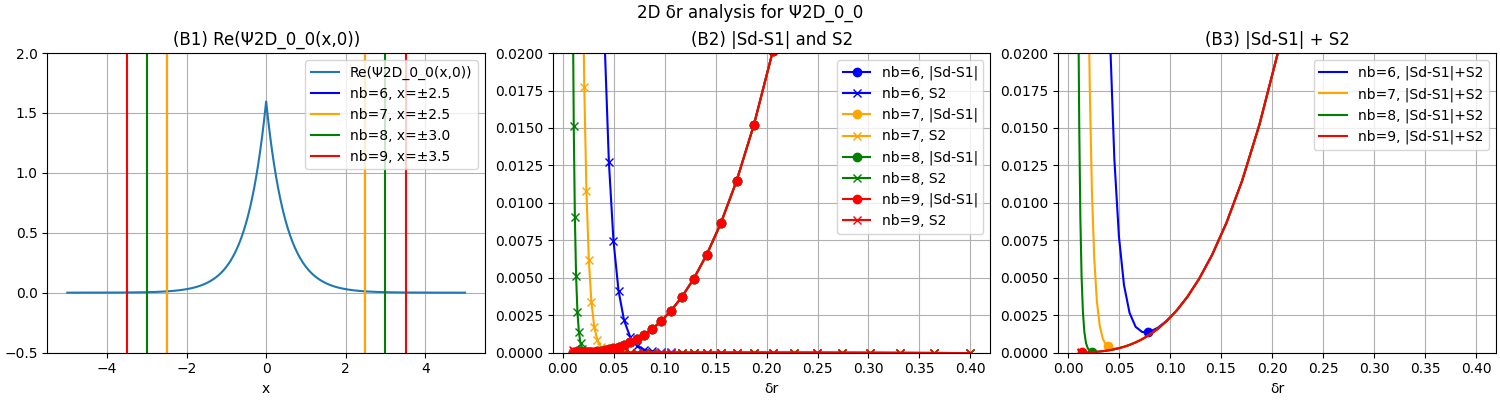
\includegraphics[width=\columnwidth]{paper2025_figs/dq_tradeoff/eval2d_dq_geom_0_0.png}
        \caption{Two-dimensional model $\PsiTwoD_{0,0}$}
        \label{subfig:dq-tradeoff-2d-0-0}
    \end{subfigure}
    \begin{subfigure}{1.0\columnwidth}
        \centering
        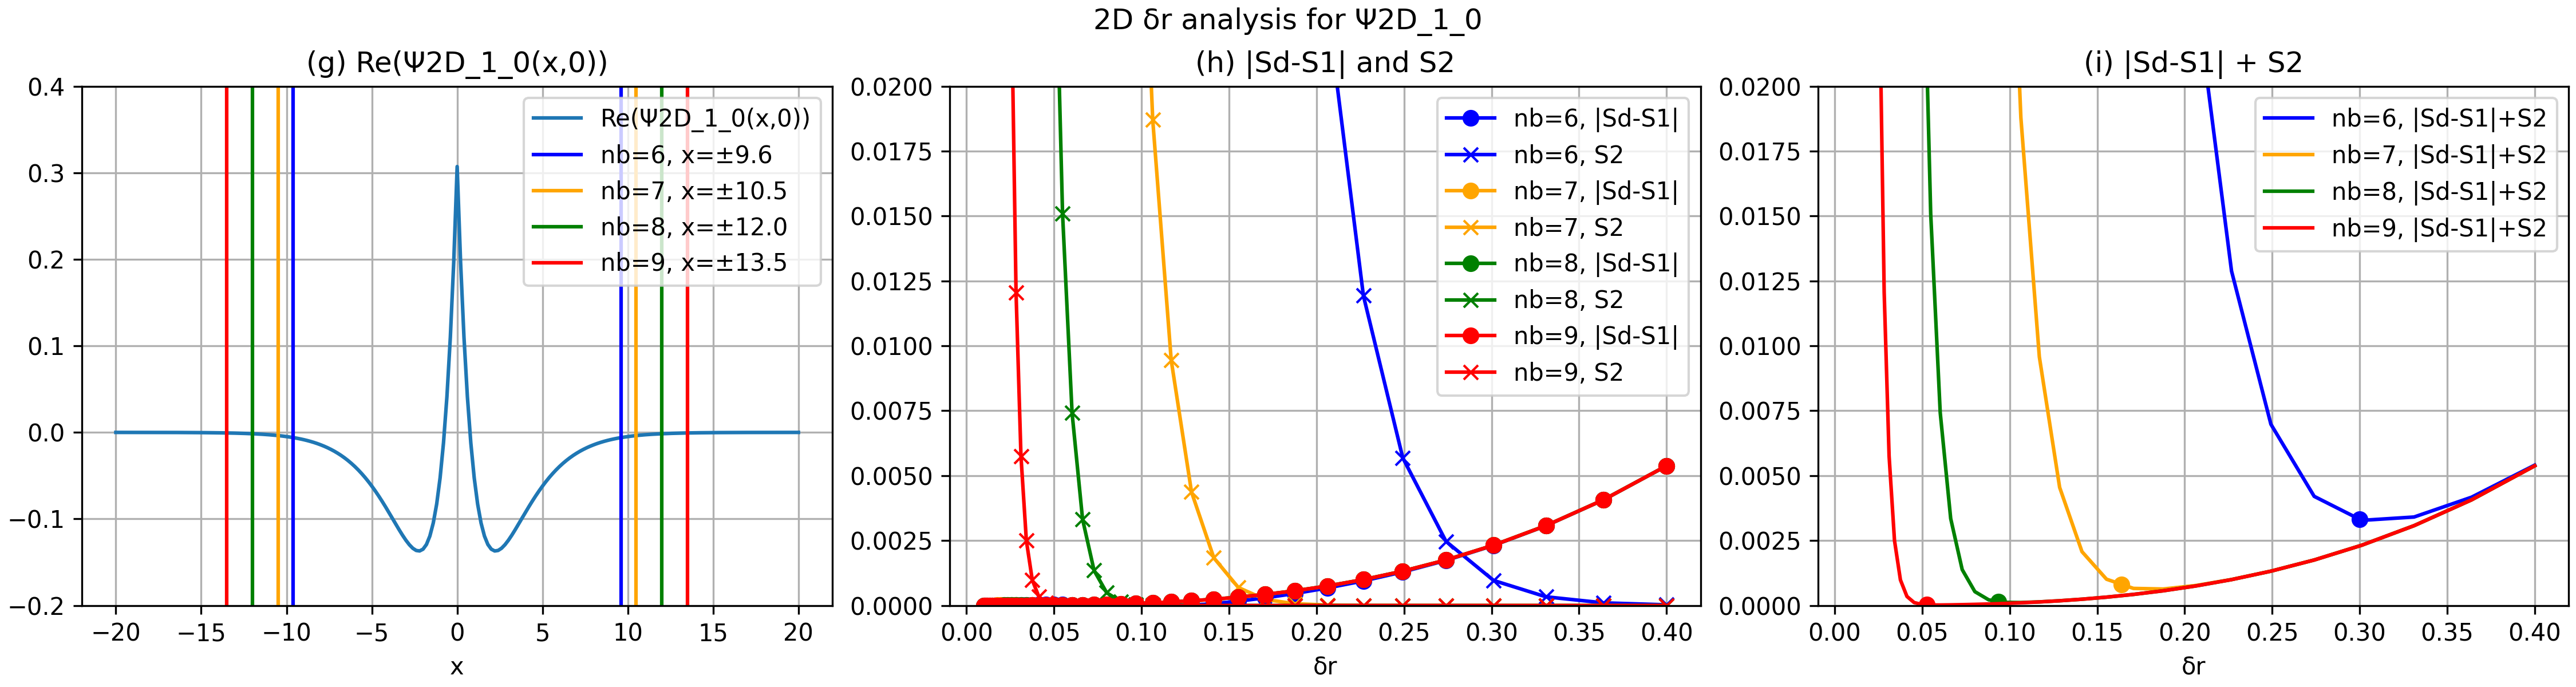
\includegraphics[width=\columnwidth]{paper2025_figs/dq_tradeoff/eval2d_dq_geom_1_0.png}
        \caption{Two-dimensional model $\PsiTwoD_{1,0}$}
        \label{subfig:dq-tradeoff-2d-1-0}
    \end{subfigure}
    \caption{Relationship between $|\Sd-S_1|$ and $S_2$ for several values of $\nb$}
    \label{fig:dq-tradeoff}
    \begin{flushleft}\small

        (a) Plot for one-dimensional $\PsiOneD_1$. (b) and (c) are plots for
        two-dimensional $\PsiTwoD_{0,0}$ and $\PsiTwoD_{1,0}$, respectively.
        (A1) through (C1) show the real part on the $y=0$ cross section of the
        wavefunction, with vertical lines indicating positions of $\pm L/2$ for
        selected $\deltar$. (A2) through (C2) plot $|\Sd-S_1|$ and $S_2$ as
        separate lines (Eqs. \eqref{eq:err-disc-definition},
        \ref{eq:err-cutoff-definition}), and (A3) through (C3) plot their sum.
        The point minimizing the sum is where the trade-off is balanced and gives
        the optimal $\deltar$ value.

    \end{flushleft}
\end{figure}
\clearpage

\subsection{Method for determining the time step}
\label{subsec:deltat-selection-method}
\subsubsection{Condition on time step Based on the Sampling Theorem}
\label{subsubsec:deltat-selection-by-sampling-theorem}
There are two bases for constraints on $\deltat$: a condition derived from the
sampling theorem and a condition derived from Trotter-decomposition error. We
first examine the sampling-theorem-based condition.

If values of the wavefunction at each step of Trotter time evolution are viewed
as sampled signals, the sampling theorem requires a sampling frequency at least
twice the highest frequency component in the signal, i.e., higher than
$1/\deltat$. In the context of Suzuki-Trotter decomposition, this means that in
both potential- and kinetic-energy terms, phase change per one time-evolution
step must be no greater than half a period, i.e., at most $\pi$.
\begin{align}
\max_{\bm{r}}\abs{\Hep(\bm{r})\deltat/\hbar} < \pi \label{eq:nyqist-limit-by-hep}\\
\max_{\bm{k}}\abs{\Hek(\bm{k})\deltat/\hbar} < \pi \label{eq:nyqist-limit-by-hek}
\end{align}
Under a given wavefunction, these expressions can be evaluated explicitly as
follows.

First, consider the one-dimensional model in this report. If one directly solves
inequality \ref{eq:nyqist-limit-by-hep} for the potential-energy term,
$\Hep$ diverges at the pole. In time-evolution calculation, we introduce an
approximation to $\Hep$ to avoid divergence, and evaluate using that
approximation.

As described in the section on Coulomb-pole treatment, the Hamiltonian
approximation for the one-dimensional model is $\HaOne(r)$ with
$\Delta_1=\deltar/2$. In terms of grid-point coordinates,
\begin{equation}
\HaOneOneD(\chij) = \begin{cases}
-\frac{1}{\abs{\chij}} & (\chij\neq0) \\
-\frac{2}{\deltar} & (\chij=0)
\end{cases}
\end{equation}
The maximum of $\abs{\HaOneOneD}$ occurs at $\chij=0$, yielding
\begin{equation}
\max_{j}\abs{\Hep(\chij)} = \frac{2\deltat}{\deltar\hbar}<\pi
\end{equation}
Solving this for $\deltat$ gives
\begin{equation}
\deltat < \frac{\pi\deltar\hbar}{2}=\frac{L\pi\hbar}{2^{\nb+1}}\equiv\deltatPmaxOneD
 \label{eq:nyqist-limit-by-hep-final}
\end{equation}
where we used $\deltar=L/2^{\nb}$.

Similarly, from inequality \eqref{eq:nyqist-limit-by-hek} for the kinetic term,
\begin{equation}
\max_{\ell}\abs{\frac{\hbar^2(\kellx)^2}{2}\cdot\frac{\deltat}{\hbar}} < \pi
\label{eq:nyqist-limit-by-hek-maximum}
\end{equation}
is obtained. The absolute value of wave number $\kaplx$ is maximal at wave-
number index $\ell=\kaplx=-2^{\nb-1}$, where
$\kellx=\kaplx\deltak=(-2^{\nb-1})\times2\pi/L$. Substituting this into
Eq. \eqref{eq:nyqist-limit-by-hek-maximum} yields
\begin{equation}
    \frac{\hbar^2}{2}\left(\frac{2\pi}{L}\cdot 2^{(\nb-1)}\right)^2\cdot\frac{\deltat}{\hbar} < \pi
\end{equation}
and solving for $\deltat$ gives
\begin{equation}
\deltat < \frac{L^2}{2^{2\nb-1}\hbar\pi}\equiv\deltatKmaxOneD
 \label{eq:nyqist-limit-by-hek-final}
\end{equation}
Using simulation duration $T$ and Trotter partition number $\nT$, with
$\deltat=T/\nT$, the corresponding lower bounds on partition count for these
upper bounds on $\deltat$ are defined as
\begin{align}
    \nTpminOneD &= \frac{T}{\deltatPmaxOneD}=\frac{2^{\nb+1}T}{L\pi\hbar}
    \label{eq:nT-pmin-definition}\\
    \nTkminOneD &= \frac{T}{\deltatKmaxOneD}=\frac{2^{2\nb-1}\pi\hbar T}{L^2}
    \label{eq:nT-kmin-definition}
\end{align}
The time-evolution partition count $\nT$ must be larger than both of these.

Next, we perform the same analysis for the two-dimensional model.

For inequality \eqref{eq:nyqist-limit-by-hep} based on the potential term, we
also use approximations for $\Hep$ in the two-dimensional model to prevent pole
divergence, as in the one-dimensional model. As discussed in the next section,
we use a common value $\deltar/4$ for parameters $\Delta_1,\Delta_2$ of
approximations $\HaOne$ and $\HaTwo$. In grid-point coordinates,
\begin{align}
\HaOneTwoD(\chij) &= \begin{cases}
    -\frac{1}{\abs{\chij}} & (\chij\neq0) \\
    -\frac{4}{\deltar} & (\chij=0)
\end{cases}\\
\HaTwoTwoD(\chij) &= -\frac{1}{\sqrt{\abs{\chij}^2+(\deltar/4)^2}}
\end{align}
Using these, the maximum value in Eq. \eqref{eq:nyqist-limit-by-hep} is
identical for both forms:
\begin{equation}
\max_{j}\abs{\HaOneTwoD(\chij)\deltat/\hbar}
  = \max_{j}\abs{\HaTwoTwoD(\chij)\deltat/\hbar}
  = \frac{4\deltat}{\deltar\hbar} < \pi
\end{equation}
which implies
\begin{equation}
\deltat < \frac{\pi\deltar\hbar}{4}
        =\frac{L\pi\hbar}{2^{\nb+2}}
        \equiv\deltatPmaxTwoD
 \label{eq:nyqist-limit-by-hep-final-2D}
\end{equation}


From inequality \eqref{eq:nyqist-limit-by-hek} based on the kinetic term,
\begin{equation}
\max_{\ell}\abs{\frac{\hbar^2((\kellx)^2+(\kelly)^2)}{2}\cdot\frac{\deltat}{\hbar}} < \pi
\label{eq:nyqist-limit-by-hek-maximum-2D}
\end{equation}
The sum of squares of wave numbers $\kellx,\kelly$ is maximal when
$\kaplx=\kaply=-2^{\nb-1}$. Using
$\kellx=\kelly=\kaplx\deltak=\kaply\deltak=-2^{\nb-1}\times2\pi/L$,
Eq. \eqref{eq:nyqist-limit-by-hek-maximum-2D} becomes
\begin{equation}
\frac{\hbar^2}{2}\cdot2\left(-\frac{2^{\nb-1}2\pi}{L}\right)^2\cdot\frac{\deltat}{\hbar}<\pi
\end{equation}
that is,
\begin{equation}
\deltat < \frac{L^2}{2^{2\nb}\hbar\pi} \equiv\deltatKmaxTwoD
 \label{eq:nyqist-limit-by-hek-final-2D}
\end{equation}
The corresponding lower bounds on Trotter partition number are
\begin{align}
    \nTpminTwoD &= \frac{T}{\deltatPmaxTwoD}=\frac{2^{\nb+2}T}{L\pi\hbar} \\
    \nTkminTwoD &= \frac{T}{\deltatKmaxTwoD}=\frac{2^{2\nb}\pi\hbar T}{L^2}
\end{align}


\subsubsection{Condition on time step Based on Trotter Error}
\label{subsec:deltat-selection-by-trotter-error}
In Trotter decomposition, error arises because the Hamiltonian is split into
kinetic and potential terms and approximated as
$e^{-it(H_1+H_2)/\hbar}\simeq\left(e^{-i{tH}_1/N}e^{-itH_2/N}\right)^N$.
Conventional Trotter error estimation uses the operator norm of the commutator
$\| [H_1,H_2] \|$, i.e.,
$\sup_{\|\psi\|=1}\|(H_1H_2-H_2H_1)\psi\|$, to bound error. This is a worst-
case estimate based on wavefunctions $\psi$ that maximize error, and has been
pointed out to overestimate errors
\cite{Childs2021.PhysRevX.11.011020}.
To obtain tighter estimates, state-dependent error evaluation assuming the
actual target wavefunction has been proposed
\cite{Burgarth2024.PhysRevResearch.6.043155}. Here we follow this proposal and
analyze based on state-dependent Trotter-error evaluation.

Unlike determination of $\deltat$ from the sampling theorem, Trotter error
formulas do not provide a specific upper bound value of $\deltat$; instead,
they provide inequalities relating $\deltat$ and error upper bounds. Let
$\phi$ be an eigenfunction of Hamiltonian $H_1+H_2$ with eigenvalue $h$, i.e.,
$\left(H_1+H_2\right)\phi=h\phi$. The error when evolving this initial state
with first-order Trotter decomposition satisfies, for any
$g\in\mathbb{R}$,
\begin{equation}
    \xiN{1}(t;\phi)=\left\|\left[\SN{1}(t)-e^{-it(H_1+H_2)/\hbar}\right]\phi\right\|
    \leq\frac{t^2}{2N}\| \left(\|(H_1-g)^2\phi\|+\|(H_2-h+g)^2\phi\|\right)
    \label{eq:observed-trotter-error-1st}
\end{equation}

\cite{Burgarth2024.PhysRevResearch.6.043155}. Here,
$\xiN{1}(t;\phi)$ is the observed error from first-order Trotter
decomposition, and $S_N^{(1)}$ is the first-order Trotter time-evolution
operator,
\begin{equation}
    \SN{1}(t)=\left(e^{-i{tH}_1/N}e^{-itH_2/N}\right)^N
\end{equation}
The minimum value of the right-hand side of
Eq. \eqref{eq:observed-trotter-error-1st} is denoted by $\BN{1}$:
\begin{equation}
\BN{1}(t;\phi)=\inf_{g\in\mathbb{R}}\frac{t^2}{2N}
    \left(\|(H_1-g)^2\phi\|+\|(H_2-h+g)^2\phi\|\right)
\label{eq:observed-trotter-error-bound-1st}
\end{equation}
Equation \eqref{eq:observed-trotter-error-bound-1st} estimates the error upper
bound for specific $t,N$, shows error order $O(t^2/N)$, and indicates inverse
proportionality to partition count $N$. However, it has been pointed out that
for small $N$ or high spatial resolution this scaling does not hold, and the
order becomes $O(t^2 N^{-1/4})$
\cite{Burgarth2024.PhysRevResearch.6.043155}。

For second-order Trotter decomposition, the error estimate is
\begin{equation}
  \xiN{2}(t;\phi)\leq\frac{t^3}{N^2}\left(\frac{1}{24}\|H_1(g)^3\phi\| + \frac{1}{8}\|H_2(g)H_1(g)^2\phi\|
  +\frac{1}{12}\|H_2(g)^3\phi\|\right)
    \label{eq:observed-trotter-error-2nd}
\end{equation}
\cite{Burgarth2024.PhysRevResearch.6.043155}. Here,
$H_1(g)=H_1-g,H_2(g)=H_2-h+g$.
The minimum value of the right-hand side of
Eq. \eqref{eq:observed-trotter-error-2nd} is denoted by $\BN{2}$:
\begin{equation}
\BN{2}(t;\phi)=\inf_{g\in\mathbb{R}}\frac{t^3}{N^2}
    \left(\frac{1}{24}\|H_1(g)^3\phi\| + \frac{1}{8}\|H_2(g)H_1(g)^2\phi\|
  +\frac{1}{12}\|H_2(g)^3\phi\|\right)
\label{eq:observed-trotter-error-bound-2nd}
\end{equation}

Among the different error types in Eq. \eqref{eq:error-total-decomposition},
when $\errtrotter$ is dominant, error reduction based on
Eqs. \eqref{eq:observed-trotter-error-1st} and
\eqref{eq:observed-trotter-error-2nd} can be expected. Conversely, if errors
other than Trotter error dominate, increasing $N$ does not yield expected
$O(N^{-1})$ or $O(N^{-2})$ reduction.


For temporal discretization parameter $\deltat$, an upper bound is set by the
sampling theorem due to use of discrete Fourier transform
(Eqs. \eqref{eq:nyqist-limit-by-hep},
\eqref{eq:nyqist-limit-by-hek-final},
\eqref{eq:nyqist-limit-by-hep-final-2D},
\eqref{eq:nyqist-limit-by-hek-final-2D}).
For Trotter error, upper bounds depend on partition number
$\nT=t/\deltat$ (Eqs. \eqref{eq:observed-trotter-error-bound-1st},
\eqref{eq:observed-trotter-error-bound-2nd}).
There is no trade-off among these constraints, but total error in
Eq. \eqref{eq:error-total-decomposition} contains multiple components, so even
if $\deltat$-related error decreases, $\errtotal$ may improve little.
From computational-cost perspective, larger $\deltat$ is preferable, so
$\deltat$ should be reduced only within the range where improvement is observed.

With time-evolution duration fixed at $t=1.0$, Figures
\ref{fig:trotter-error-t1-part1} and
\ref{fig:trotter-error-t1-part2} show error upper bounds
$\BN{\gamma}(\psi;t)$ and observed errors $\xiN{\gamma}$ as Trotter partition
count $\nT$ varies, where $\gamma=1,2$ denotes Trotter order. As an example of
longer simulation time, considering that period of wavefunction
$\PsiTwoD_{1,0}$ is $2\pi/E_2=28.277$, plots for $t=30.0$ are shown in
Figures \ref{fig:trotter-error-t30-part1} and
\ref{fig:trotter-error-t30-part2}. Vertical lines indicate lower bounds
$\nTpminTwoD$ and $\nTkminTwoD$ from the sampling theorem. Unlike other plots in
energy units, these plots show norms of wavefunction-amplitude differences
defined in Eqs. \eqref{eq:observed-trotter-error-1st} and
\eqref{eq:observed-trotter-error-2nd}.

Differences due to Trotter order $\gamma$ were barely observed in examples with
azimuthal quantum number $m=0$, namely $\PsiTwoD_{0,0}$ and $\PsiTwoD_{1,0}$
(Figures \ref{subfig:trotter-error-2d-0-0-6b-t1} to
\ref{subfig:trotter-error-2d-1-0-9b-t1}). For $\PsiTwoD_{1,1}$ with $m=1$,
differences appeared in the low-$\nT$ region. Burgarth reported that in a
three-dimensional hydrogen model, increasing Trotter order does not improve
accuracy for eigenfunctions with azimuthal quantum number 0
\cite{Burgarth2024.PhysRevResearch.6.043155}. Although dimensionality differs,
our examples with $\PsiTwoD_{0,0}$ and $\PsiTwoD_{1,0}$ show similar behavior.

In all plots, both $\xiN{1}$ and $\xiN{2}$ decrease as $\nT$ increases, but
saturate around $\nT=\nTkminTwoD$. For $\PsiTwoD_{1,1}$, a slight additional
decrease is observed for $\nT>\nTkminTwoD$, but it is small. This is likely
because in that region the spatial-resolution error component $\errdisc$ is
dominant. For the wavefunctions shown here, setting $\nT$ larger than
$\nTkminTwoD$ does not improve error. For example, comparing
Figures \ref{subfig:trotter-error-2d-0-0-6b-t1} and
\ref{subfig:trotter-error-2d-0-0-9b-t1}, for the same $\PsiTwoD_{0,0}$,
increasing $n_b$ from 6 to 9 reduces the saturated error by about one order of
magnitude.

Note that the corresponding $\deltat$ values for these $\nT$ values are
sub-attosecond, since $t=1.0\ \mathrm{a.u.}=24.19\ \mathrm{attosecond}
(\mathrm{as})$ is further divided into approximately $10^2$ to $10^3$ intervals.

\begin{figure}[ht]
    \centering
    \begin{subfigure}{0.45\columnwidth}
        \centering
        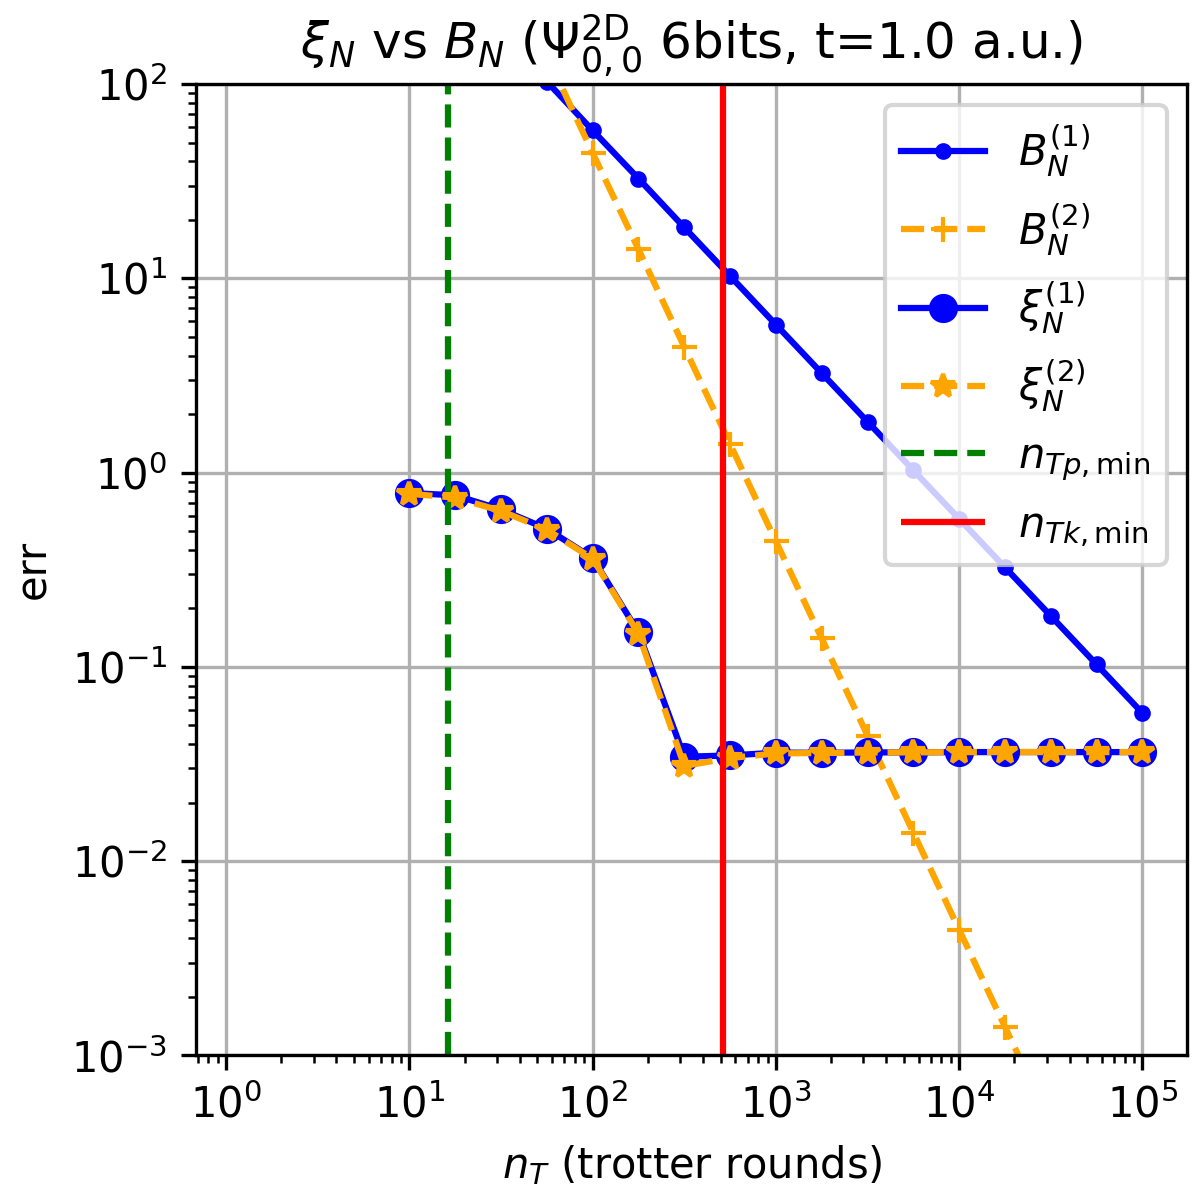
\includegraphics[width=1\columnwidth]{paper2025_figs/sdt_error/trotter_err_n0_m0_6b_t1.0.png}
        \caption{$\PsiTwoD_{0,0}, \nb=6, t=1.0$}
        \label{subfig:trotter-error-2d-0-0-6b-t1}
    \end{subfigure}
    \begin{subfigure}{0.45\columnwidth}
        \centering
        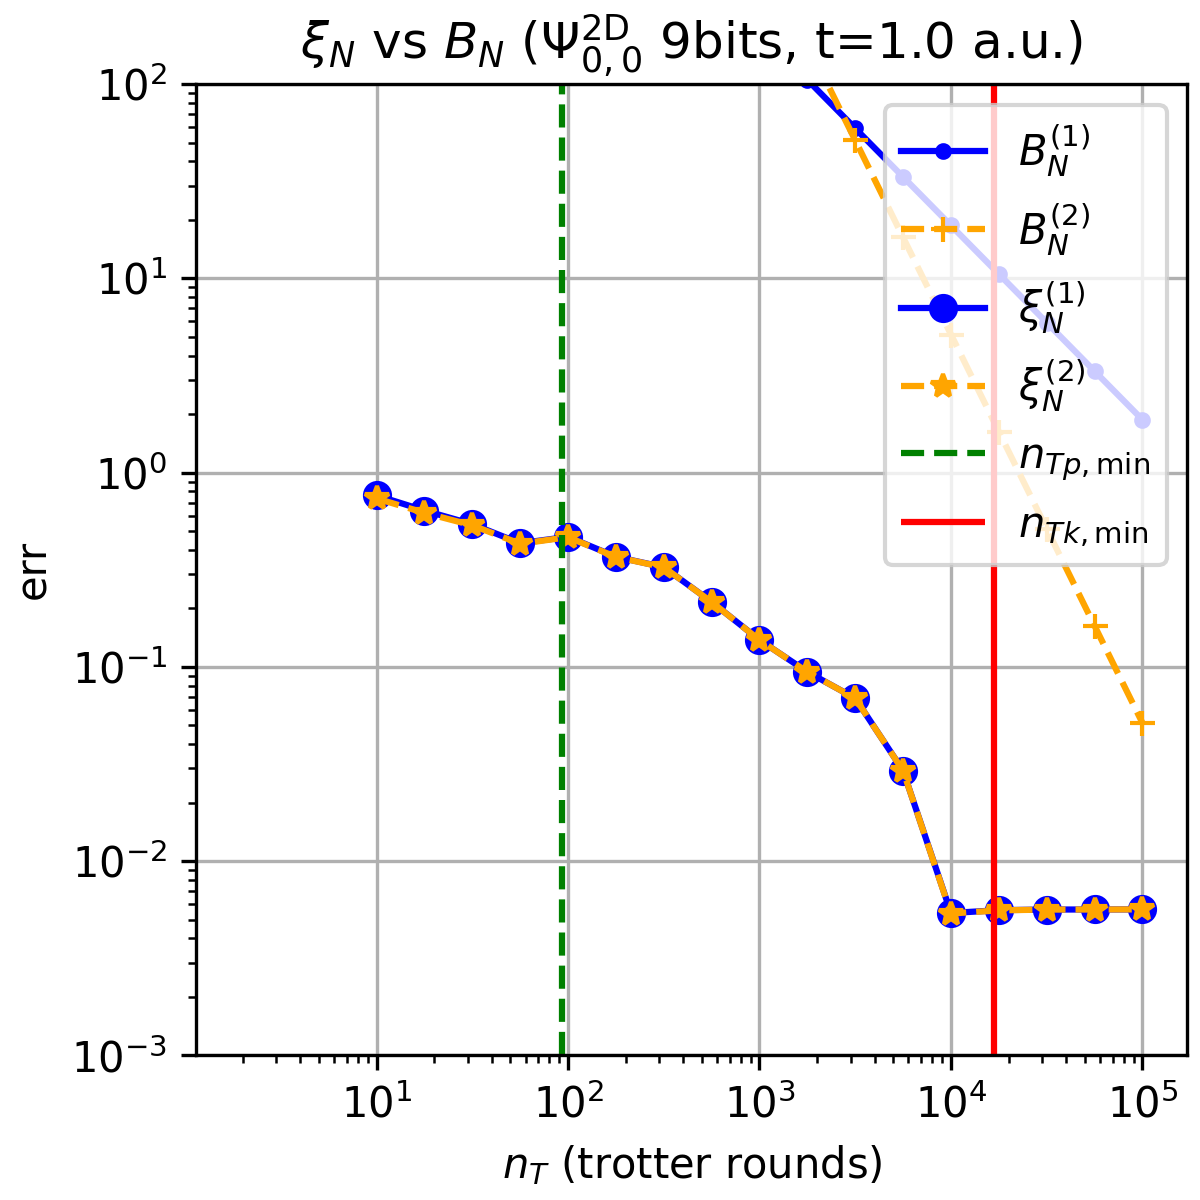
\includegraphics[width=1\columnwidth]{paper2025_figs/sdt_error/trotter_err_n0_m0_9b_t1.0.png}
        \caption{$\PsiTwoD_{0,0}, \nb=9, t=1.0$}
        \label{subfig:trotter-error-2d-0-0-9b-t1}
    \end{subfigure}

    \begin{subfigure}{0.45\columnwidth}
        \centering
        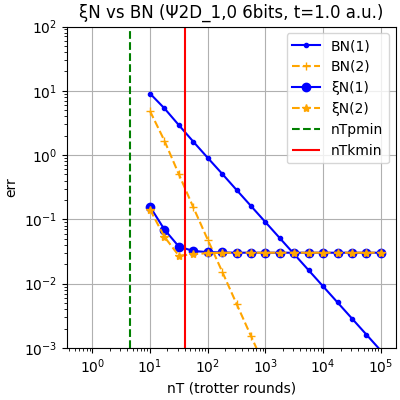
\includegraphics[width=1\columnwidth]{paper2025_figs/sdt_error/trotter_err_n1_m0_6b_t1.0.png}
        \caption{$\PsiTwoD_{1,0}, \nb=6, t=1.0$}
        \label{subfig:trotter-error-2d-1-0-6b-t1}
    \end{subfigure}
    \begin{subfigure}{0.45\columnwidth}
        \centering
        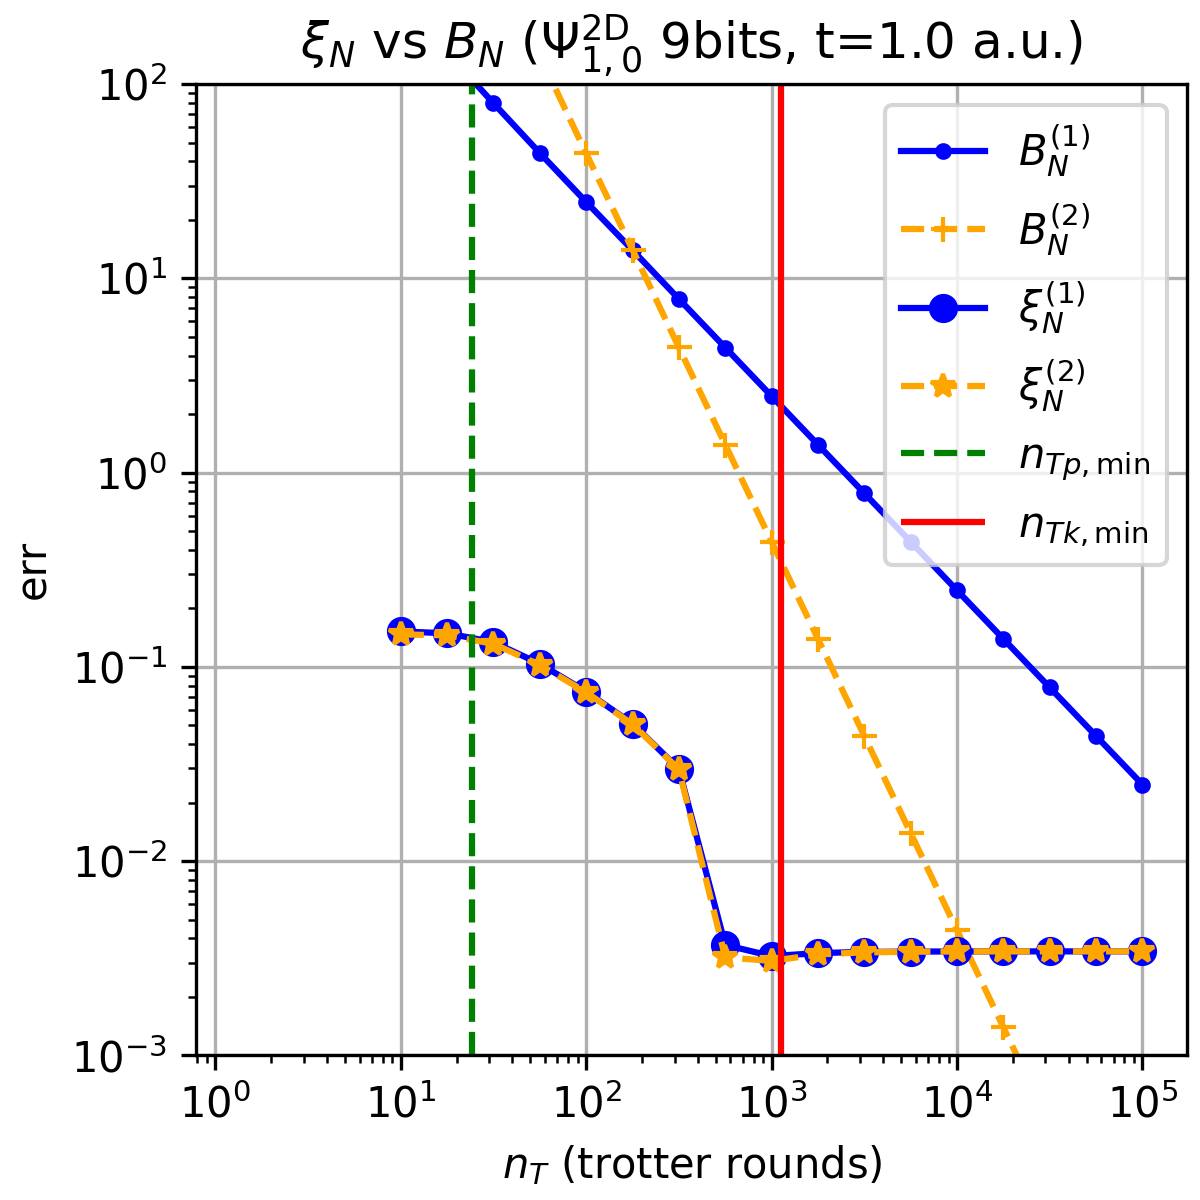
\includegraphics[width=1\columnwidth]{paper2025_figs/sdt_error/trotter_err_n1_m0_9b_t1.0.png}
        \caption{$\PsiTwoD_{1,0}, \nb=9, t=1.0$}
        \label{subfig:trotter-error-2d-1-0-9b-t1}
    \end{subfigure}

    \caption{Upper error bound $\BN{\gamma}$ and observed value $\xiN{\gamma}$ versus partition count $\nT$ for time-evolution duration $t=1.0$}
    \label{fig:trotter-error-t1-part1}
    \begin{flushleft}\small

        Error versus Trotter partition count for two-dimensional-model
        wavefunctions. Time-evolution duration $t=1.0$ is fixed, and the
        horizontal axis is partition count $\nT$. $\xiN{1}$ and $\xiN{2}$ are
        errors for Trotter orders 1 and 2, respectively (Eqs.
        \eqref{eq:observed-trotter-error-1st},
        \eqref{eq:observed-trotter-error-2nd}). These values include error
        components other than Trotter error. $\BN{1}$ and $\BN{2}$ are analytical
        upper bounds of Trotter error (Eqs.
        \eqref{eq:observed-trotter-error-bound-1st},
        \eqref{eq:observed-trotter-error-bound-2nd}). Vertical lines
        $\nT=\nTpminTwoD$ and $\nT=\nTkminTwoD$ are Trotter partition counts
        corresponding to sampling-theorem-based upper bounds
        $\deltatPmaxTwoD$ and $\deltatKmaxTwoD$, respectively
        (Eqs. \eqref{eq:nT-pmin-definition}, \eqref{eq:nT-kmin-definition}).

    \end{flushleft}
\end{figure}

\begin{figure}[ht]
    \centering
    \begin{subfigure}{0.45\columnwidth}
        \centering
        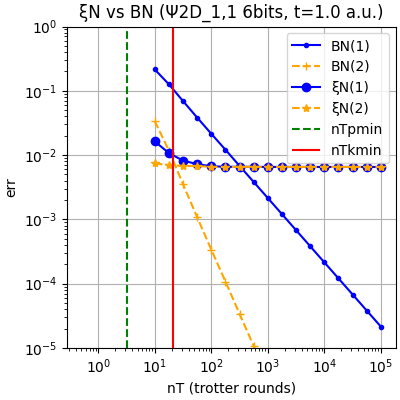
\includegraphics[width=1\columnwidth]{paper2025_figs/sdt_error/trotter_err_n1_m1_6b_t1.0.png}
        \caption{$\PsiTwoD_{1,1}, \nb=6, t=1.0$}
        \label{subfig:trotter-error-2d-1-1-6b-t1}
    \end{subfigure}
    \begin{subfigure}{0.45\columnwidth}
        \centering
        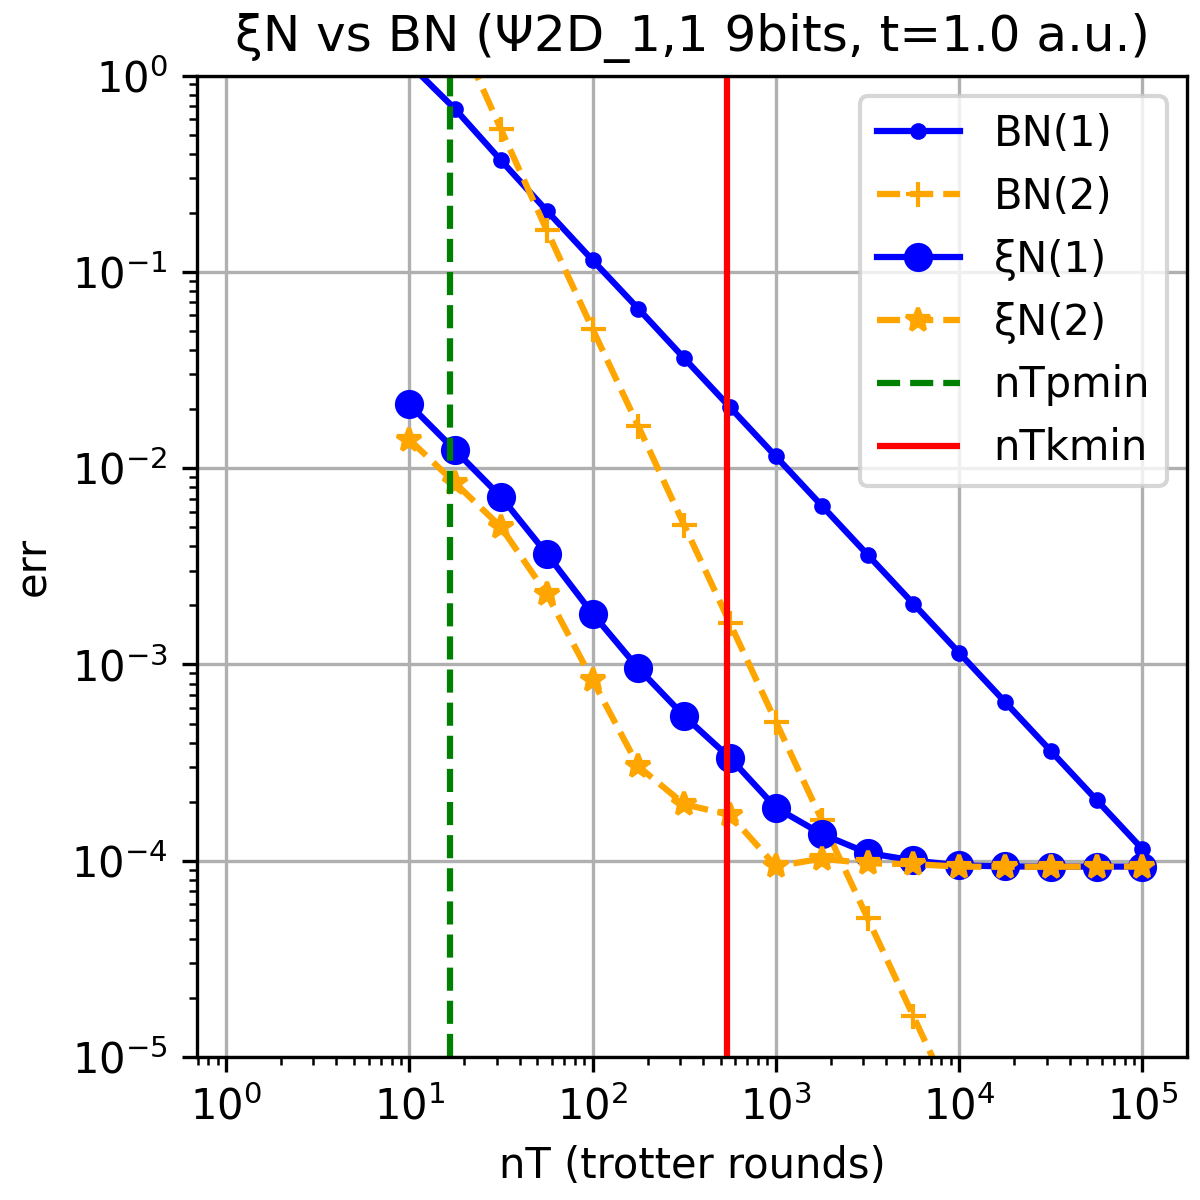
\includegraphics[width=1\columnwidth]{paper2025_figs/sdt_error/trotter_err_n1_m1_9b_t1.0.png}
        \caption{$\PsiTwoD_{1,1}, \nb=9, t=1.0$}
        \label{subfig:trotter-error-2d-1-1-9b-t1}
    \end{subfigure}
    \caption{Upper error bound $\BN{\gamma}$ and observed value $\xiN{\gamma}$ versus partition count $\nT$ for time-evolution duration $t=1.0$}
    \label{fig:trotter-error-t1-part2}
    \begin{flushleft}\small

        Error versus Trotter partition count for two-dimensional-model
        wavefunctions (continued).
    \end{flushleft}
\end{figure}

\begin{figure}[ht]
    \centering
    \begin{subfigure}{0.45\columnwidth}
        \centering
        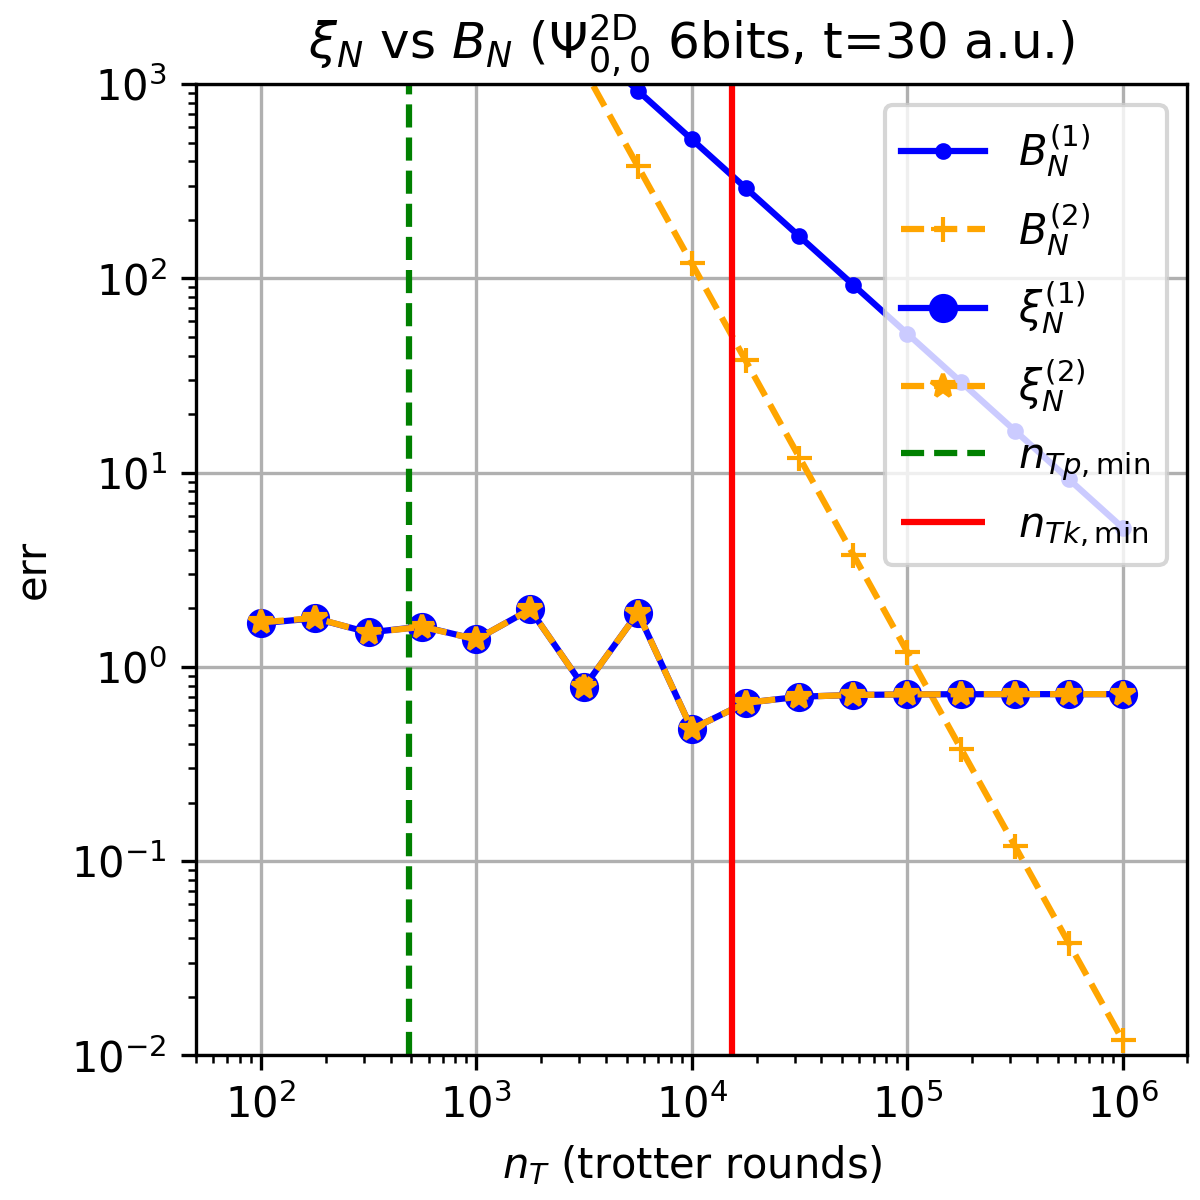
\includegraphics[width=1\columnwidth]{paper2025_figs/sdt_error/trotter_err_n0_m0_6b_t30.png}
        \caption{$\PsiTwoD_{0,0}, \nb=6, t=30.0$}
        \label{subfig:trotter-error-2d-0-0-6b-t30}
    \end{subfigure}
    \begin{subfigure}{0.45\columnwidth}
        \centering
        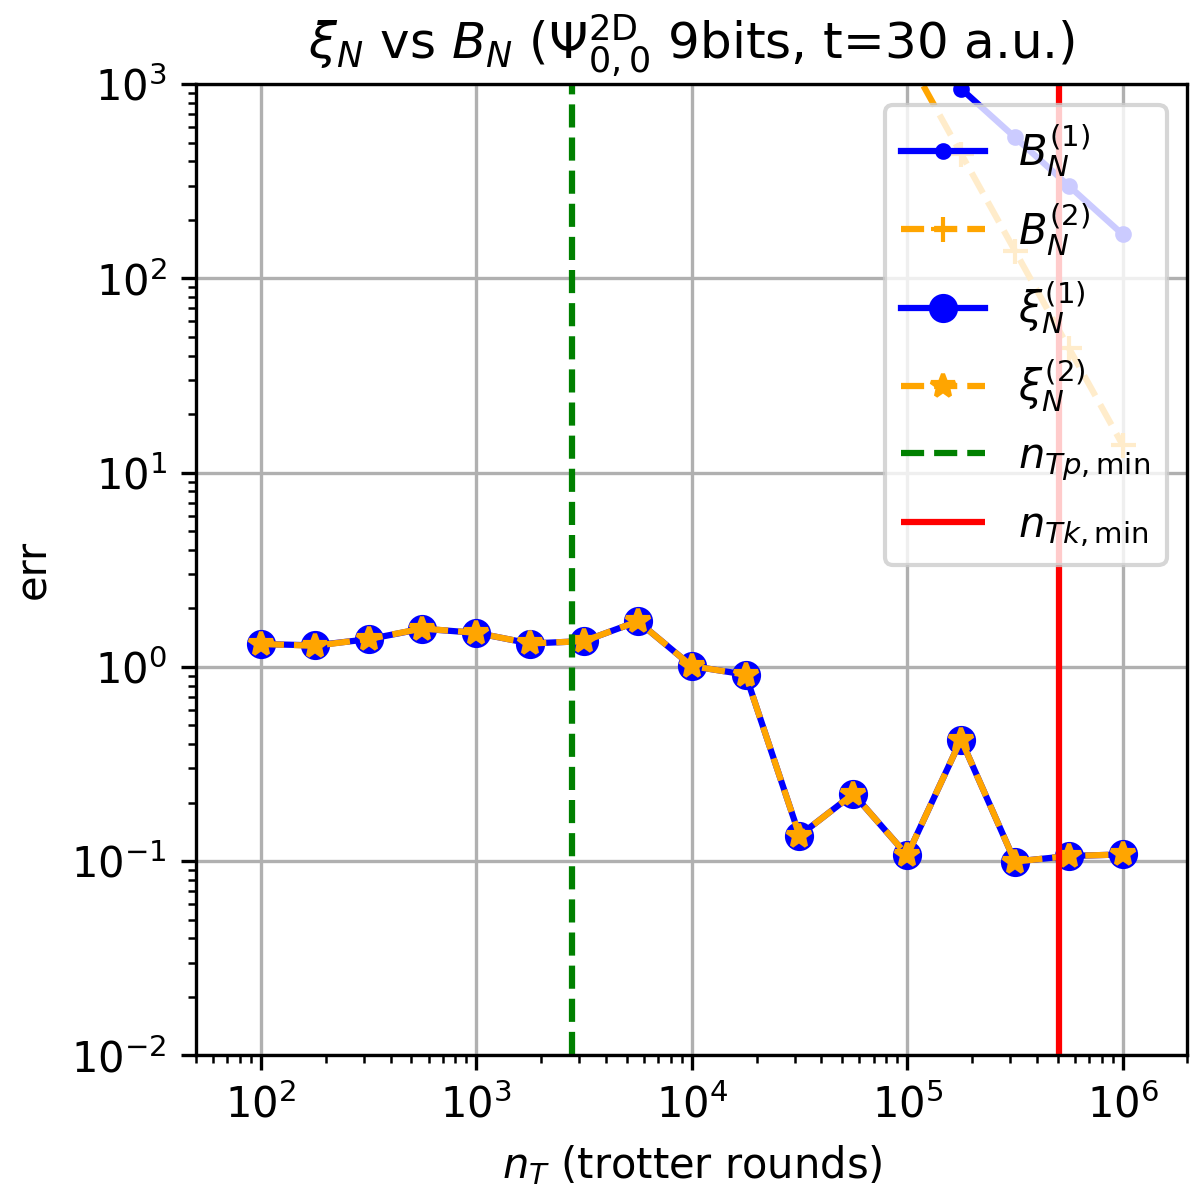
\includegraphics[width=1\columnwidth]{paper2025_figs/sdt_error/trotter_err_n0_m0_9b_t30.png}
        \caption{$\PsiTwoD_{0,0}, \nb=9, t=30.0$}
        \label{subfig:trotter-error-2d-0-0-9b-t30}
    \end{subfigure}

    \begin{subfigure}{0.45\columnwidth}
        \centering
        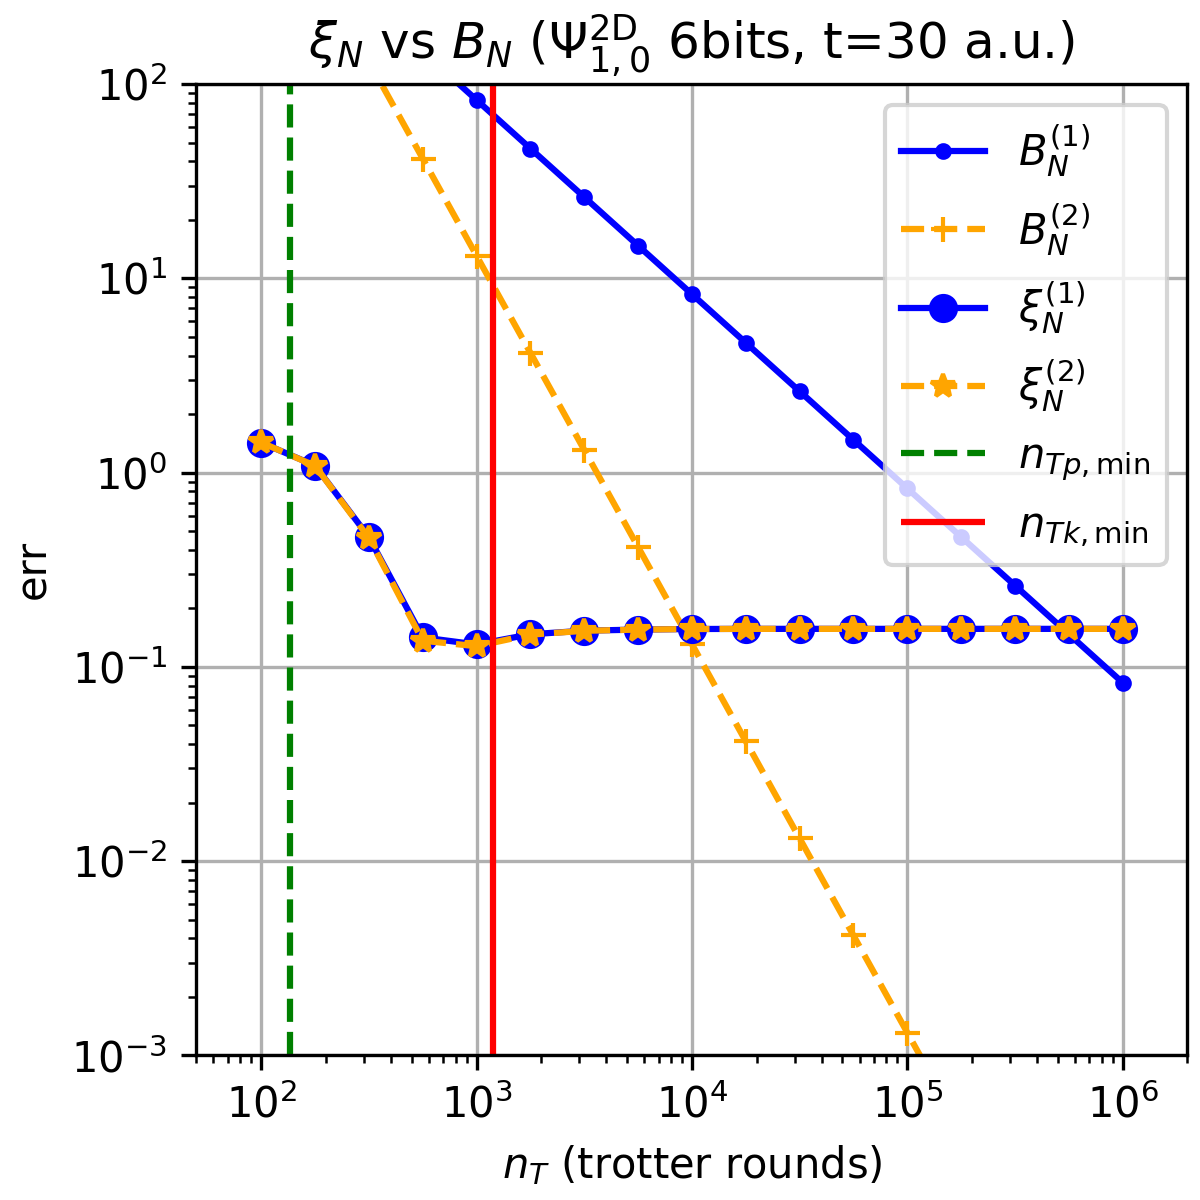
\includegraphics[width=1\columnwidth]{paper2025_figs/sdt_error/trotter_err_n1_m0_6b_t30.png}
        \caption{$\PsiTwoD_{1,0}, \nb=6, t=30.0$}
        \label{subfig:trotter-error-2d-1-0-6b-t30}
    \end{subfigure}
    \begin{subfigure}{0.45\columnwidth}
        \centering
        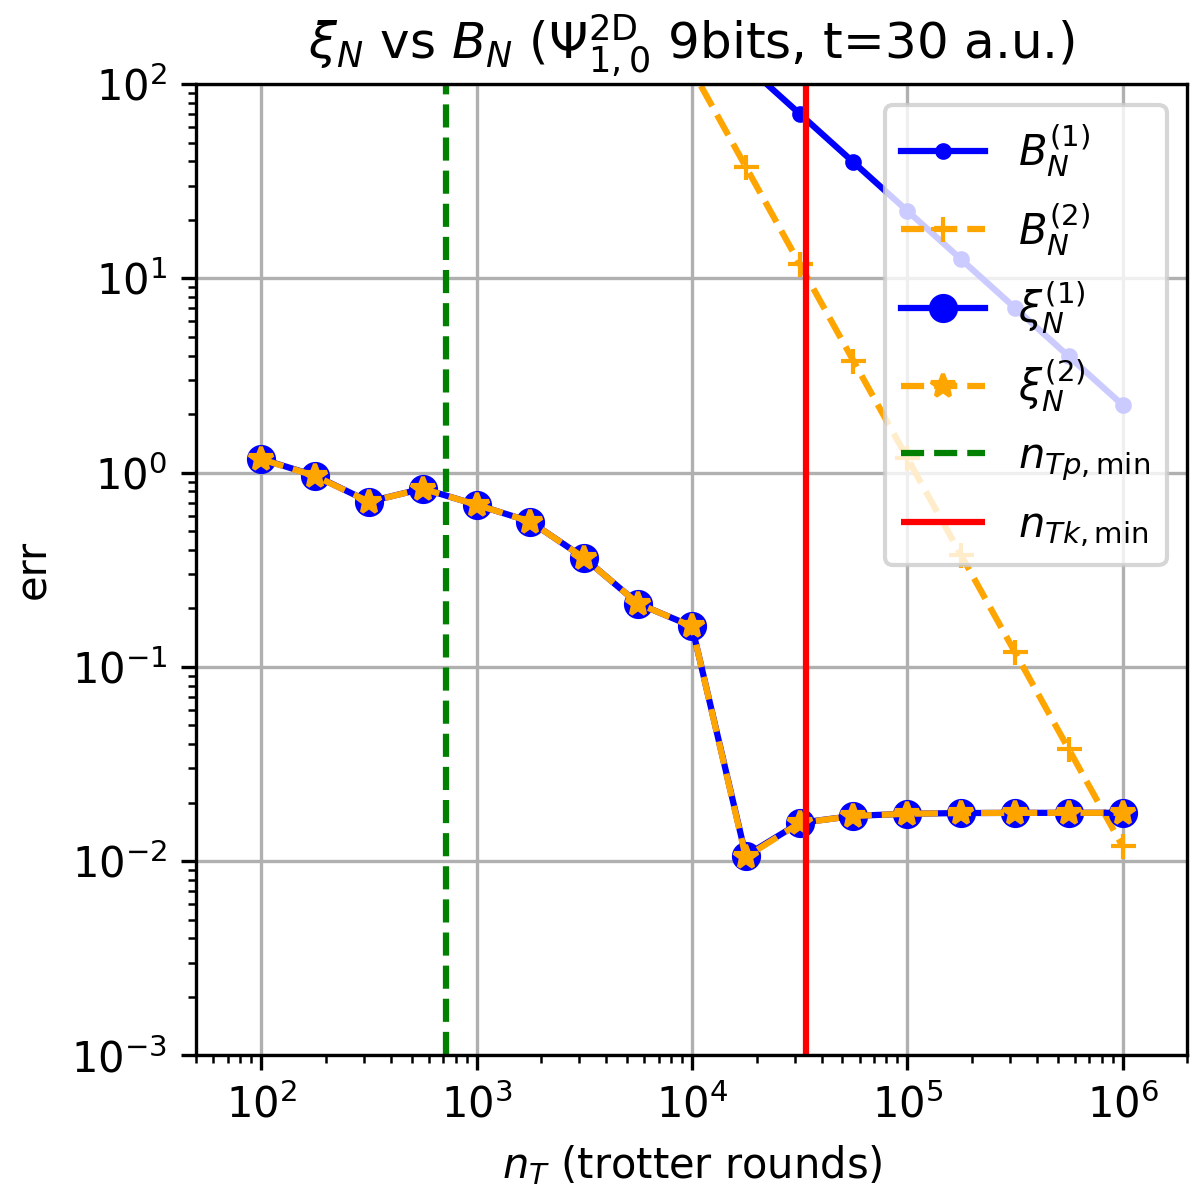
\includegraphics[width=1\columnwidth]{paper2025_figs/sdt_error/trotter_err_n1_m0_9b_t30.png}
        \caption{$\PsiTwoD_{1,0}, \nb=9, t=30.0$}
        \label{subfig:trotter-error-2d-1-0-9b-t30}
    \end{subfigure}

    \caption{Upper error bound $\BN{\gamma}$ and observed value $\xiN{\gamma}$ versus partition count $\nT$ for time-evolution duration $t=30.0$}
    \label{fig:trotter-error-t30-part1}
\end{figure}

\begin{figure}[ht]
    \centering
    \begin{subfigure}{0.45\columnwidth}
        \centering
        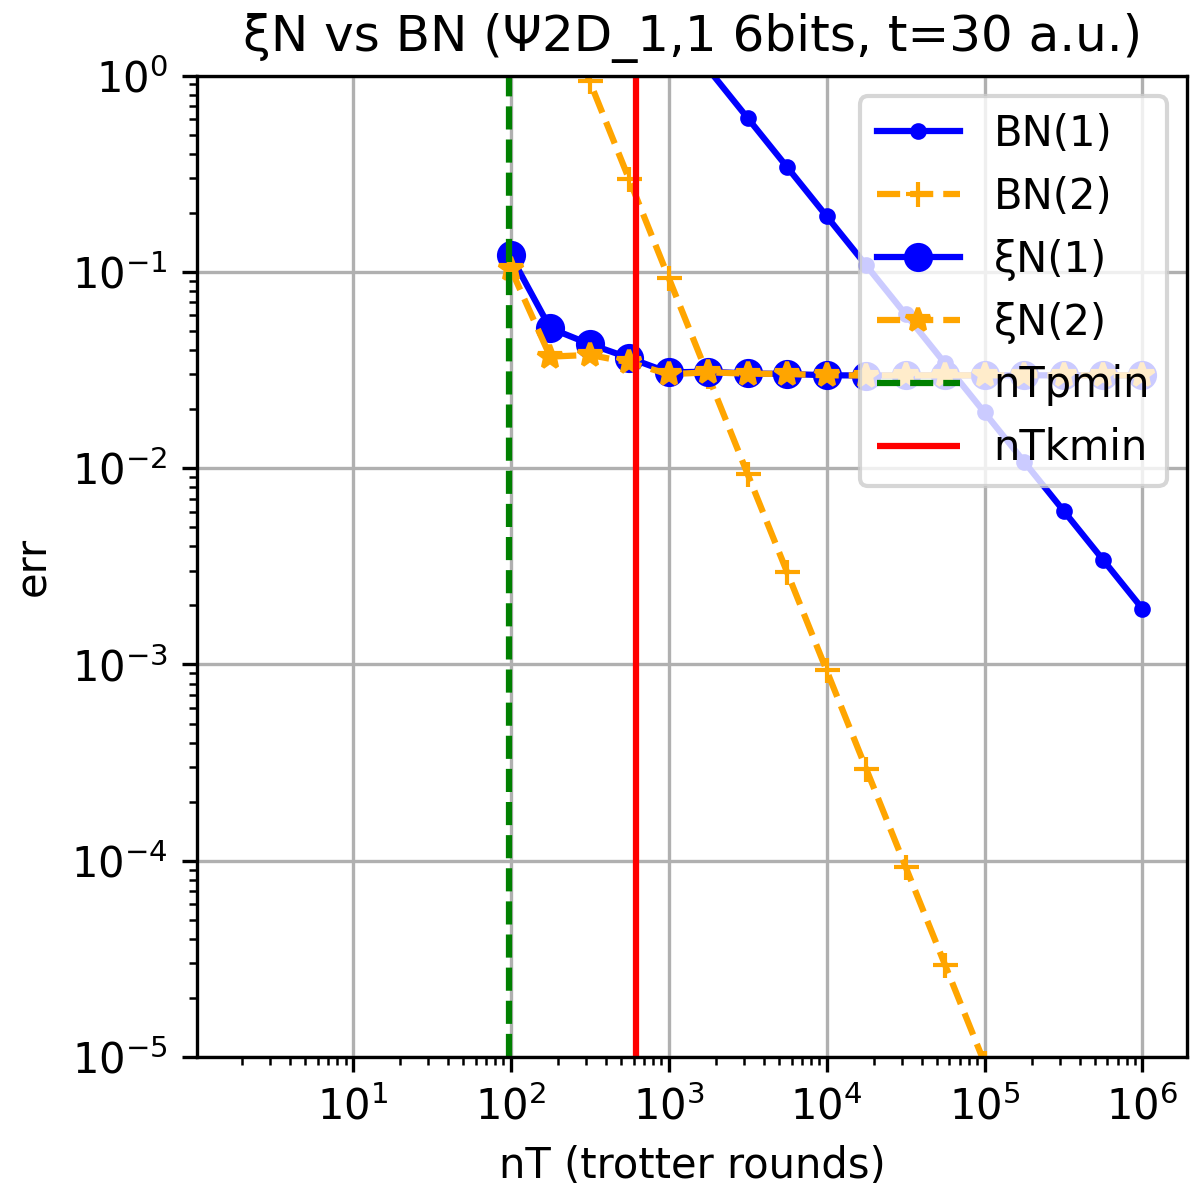
\includegraphics[width=1\columnwidth]{paper2025_figs/sdt_error/trotter_err_n1_m1_6b_t30.png}
        \caption{$\PsiTwoD_{1,1}, \nb=6, t=30.0$}
        \label{subfig:trotter-error-2d-1-1-6b-t30}
    \end{subfigure}
    \begin{subfigure}{0.45\columnwidth}
        \centering
        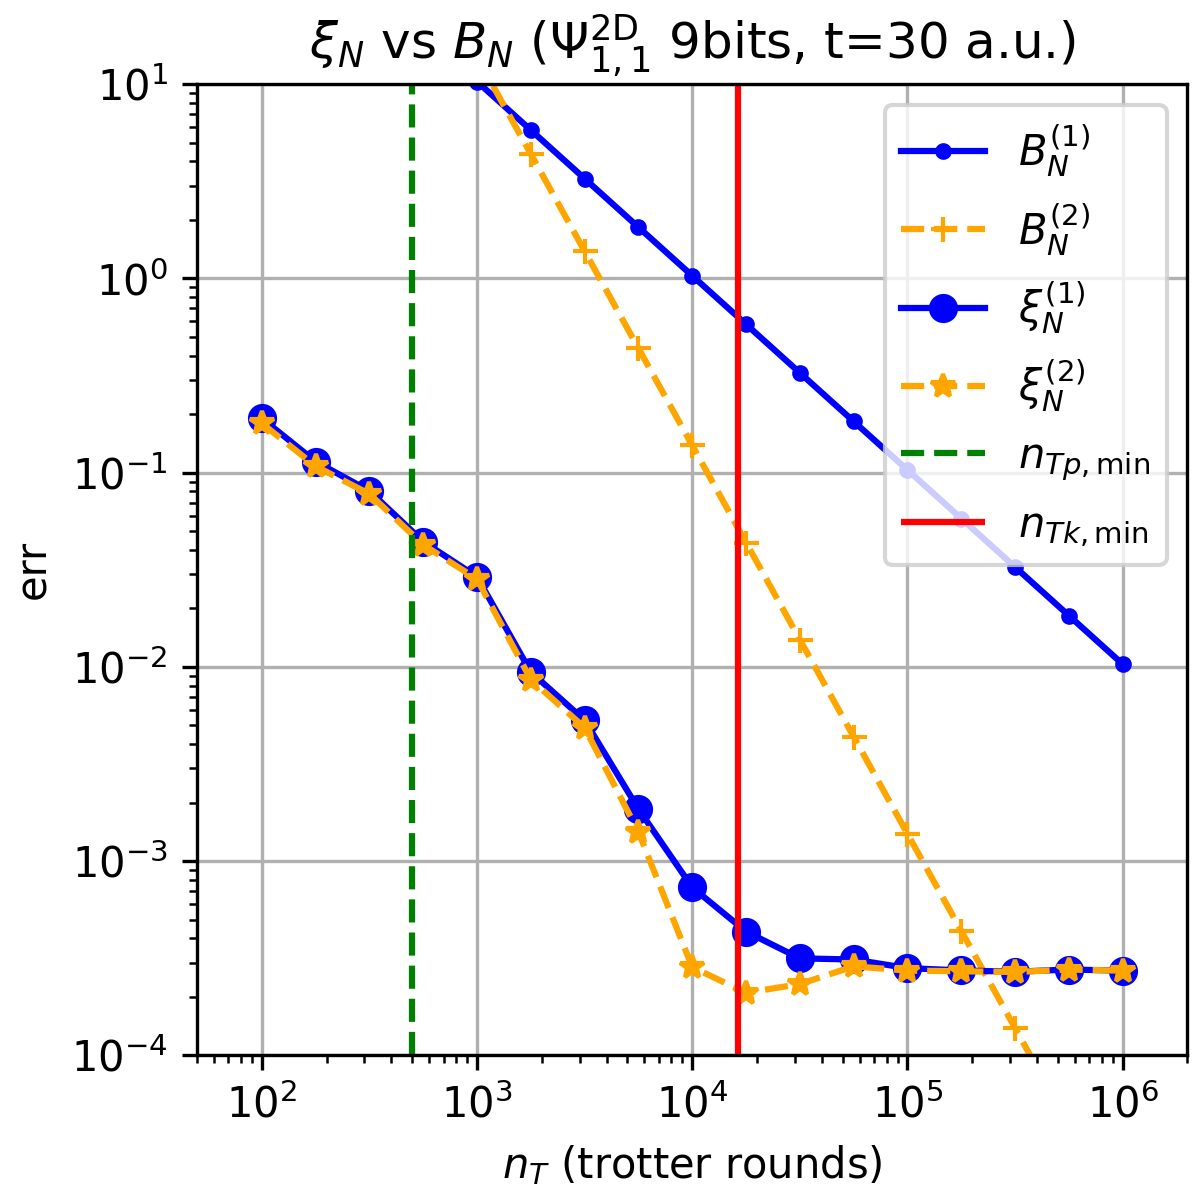
\includegraphics[width=1\columnwidth]{paper2025_figs/sdt_error/trotter_err_n1_m1_9b_t30.png}
        \caption{$\PsiTwoD_{1,1}, \nb=9, t=30.0$}  
        \label{subfig:trotter-error-2d-1-1-9b-t30}
    \end{subfigure}

    \caption{Upper error bound $\BN{\gamma}$ and observed value $\xiN{\gamma}$ versus partition count $\nT$ for time-evolution duration $t=30.0$ (continued)}
    \label{fig:trotter-error-t30-part2}
\end{figure}
\clearpage

\section{Conclusion}
In this study, for a two-dimensional hydrogen-atom model, we presented a circuit
configuration that enables full-system time evolution on a Qiskit emulator. To
the best of our investigation, this is the first example in which grid-based
time-evolution calculation, including Coulomb-potential evaluation, was
implemented in quantum circuits and executed on an emulator.

As a method for handling Coulomb-potential singularities, we proposed using
$r_{\mathrm{eff}}=\delta r/4$ as the representative interparticle distance in
grid cells containing the pole for the two-dimensional model. Within the range
of numerical evaluations performed, this value minimized error.

To minimize error under a given qubit budget, we proposed determining grid
spacing $\delta r$ from the trade-off between discretization and cutoff errors.
We also confirmed, within the numerical range evaluated, that Trotter time step
$\delta t$ can be determined based on the sampling theorem by focusing on the
rate of temporal phase change of the highest-frequency component in the
wavefunction’s momentum representation. Furthermore, for ground-state
wavefunctions, when these constraints are satisfied, remaining errors were
dominated by non-Trotter components.

These findings provide useful guidance for setting simulation conditions in
grid-based methods.


\printbibliography[heading=bibintoc, title={References}]

%%%%%%%%%%%%%%%% Appendix

\appendix
\section{Derivation of Delta 1 for the Potential Approximation}
\label{chap:appendix_derivation_derivation}

This appendix presents the derivation of parameter $\Delta_1$ in approximation
$HaOne(r)$ described in Section \ref{sec:coulomb-potential-handling}.

First, we derive Eq. \eqref{eq:delta-1-0-0} for parameter
$\Delta_{1,0,0}$ associated with $\PsiTwoD_{0,0}$.

The integral $W_{0,0}$ is
\begin{align}
  W_{0,0}
   &= \int_{r=0}^{\deltar/2}\int_{\theta=0}^{2\pi}
      \Hep(r)\abs{\PsiTwoD_{0,0}(r)}^2rd\theta dr\notag\\
   &= \int_{r=0}^{\deltar/2}\int_{\theta=0}^{2\pi}
      -\frac{1}{r}\left(\frac{q_0^3(0-\abs{0})!}{\pi(0+\abs{0})!}\right)
      (2q_0r)^{2\abs{0}}\exp(-2q_0r)
      \left[L_{0-\abs{0}}^{2\abs{0}}(2q_0r)\right]^2 rd\theta dr\notag\\
   &= -2\pi\int_{r=0}^{\deltar/2}\frac{q_0^3}{\pi}\frac{1}{r}e^{-2q_0r}r\ dr=-2q_0^3
      \left[-\frac{1}{2q_0}e^{-2q_0r}\right]_{0}^{\deltar/2}\notag\\
   &=-q_0^2(-e^{-q_0\deltar}+1)
\end{align}
For comparison, $W_{0,0}^\prime$ is
\begin{align}
    W_{0,0}^\prime
    &=\pi\left(\frac{\deltar}{2}\right)^2
       \HaOne(0)\abs{\PsiTwoD_{0,0}(0)}^2\notag\\
    &=\frac{\pi\deltar^2}{4}\left(-\frac{1}{\Delta_1}\right)
    \left(\frac{q_0^3(0-\abs{0})!}{\pi(0+\abs{0})!}\right)
    (0)^{2\abs{0}}\exp(0)\left[L_{0-\abs{0}}^{2\abs{0}}(0)\right]^2\notag\\
    &= -\frac{\pi\deltar^2q_0^3}{4\pi\Delta_1}\notag\\
    &= -\frac{\deltar^2q_0^3}{4\Delta_1}
\end{align}
Solving $W_{0,0}=W_{0,0}^\prime$ gives
\begin{equation}
-q_0^2\left(-e^{-q_0\deltar}+1\right)=-\frac{\deltar^2q_0^3}{4\Delta_1}
\end{equation}
\begin{align}
\Delta_1&=\frac{\deltar^2q_0}{4\left(-e^{-q_0\deltar}+1\right)}\notag\\
&\simeq\frac{\deltar^2q_0}{4\left(-(1-q_0\deltar)+1\right)}\notag\\
&=\frac{\deltar}{4}
\end{align}


Next, we derive Eq. \eqref{eq:delta-1-1-0} for parameter
$\Delta_{1,1,0}$ associated with $\PsiTwoD_{1,0}$.

Computing $W_{1,0}$ and $W_{1,0}^\prime$ respectively, $W_{1,0}$ is
\begin{align}
  W_{1,0}
   &= \int_{r=0}^{\deltar/2}\int_{\theta=0}^{2\pi}
      \Hep(r)\abs{\PsiTwoD_{1,0}(r)}^2rd\theta dr\notag\\
   &= \int_{r=0}^{\deltar/2}\int_{\theta=0}^{2\pi}
      -\frac{1}{r}\left(\frac{q_0^3(1-\abs{0})!}{\pi(1+\abs{0})!}\right)
      (2q_0r)^{2\abs{0}}\exp(-2q_0r)
      \left[L_{1-\abs{0}}^{2\abs{0}}(2q_0r)\right]^2 rd\theta dr\notag\\
   &= -2\pi\int_{r=0}^{\deltar/2}\frac{q_0^3}{\pi}e^{-2q_0r}(1-2q_0r)^2dr\notag\\
   &= -2q_0^3\left[\left(-\frac{1}{2q_0}+2q_0r^2\right)e^{-2q_0r}\right]_{0}^{\deltar/2} \notag\\
   &= -2q_0^3\left\{\left(-\frac{1}{2q_0}+\frac{q_0\deltar^2}{2}\right)e^{-q_0\deltar}+\frac{1}{2q_0}\right\}\notag\\
   &= q_0^2\left\{\left(1-q_0^2\deltar^2\right)e^{-q_0\deltar}-1\right\}
\end{align}
For comparison, $W_{1,0}^\prime$ is
\begin{align}
    W_{1,0}^\prime
    &=\pi\left(\frac{\deltar}{2}\right)^2
         \HaOne(0)\abs{\PsiTwoD_{1,0}(0)}^2\notag\\
    &=\frac{\pi\deltar^2}{4}\left(-\frac{1}{\Delta_1}\right)
    \left(\frac{q_0^3(1-\abs{0})!}{\pi(1+\abs{0})!}\right)
    (0)^{2\abs{0}}\exp(0)\left[L_{1-\abs{0}}^{2\abs{0}}(0)\right]^2\notag\\
    &= -\frac{\pi\deltar^2q_0^3}{4\pi\Delta_1}\notag\\
    &= -\frac{\deltar^2q_0^3}{4\Delta_1}
\end{align}
Solving $W_{1,0}=W_{1,0}^\prime$ gives
\begin{equation}
q_0^2\left\{\left(1-q_0^2\deltar^2\right)e^{-q_0\deltar}-1\right\}
=-\frac{\deltar^2q_0^3}{4\Delta_1}
\end{equation}
\begin{align}
\Delta_1&=\frac{\deltar^2q_0}{4\left\{\left(1-q_0^2\deltar^2\right)e^{-q_0\deltar}-1\right\}}\notag\\
&\simeq-\frac{\deltar^2q_0}{4\left\{\left(1-q_0^2\deltar^2\right)(1-q_0\deltar)-1\right\}}\notag\\
&=-\frac{\deltar^2q_0}{4\left(1-q_0^2\deltar^2-q_0\deltar+q_0^3\deltar^3-1\right)}\notag\\
&\simeq\frac{\deltar}{4}
\end{align}
is obtained.


\end{document}